% !TeX encoding = UTF-8
% !TeX root = master.tex
% !TeX spellcheck = en_US

\documentclass[a4paper,twoside]{article}

\usepackage[utf8]{inputenc}
\usepackage[T1]{fontenc}
\usepackage[english]{babel}
\selectlanguage{english}
\usepackage{amsmath}
\usepackage{algorithm}
\usepackage[noend]{algpseudocode}
\usepackage{graphicx}
\usepackage{grffile}
\graphicspath{{figures/}}
\usepackage{subfigure}
\usepackage{float}
\usepackage{booktabs}
\usepackage{tabu}
\usepackage{rotating}
\usepackage{array}
\usepackage{multicol}
\usepackage{multirow}
\usepackage{url}
\usepackage{footnote}
\usepackage{footmisc}
\usepackage[hidelinks]{hyperref} %[draft,hidelinks]
\usepackage[all]{hypcap}
\usepackage[capitalise,noabbrev,nameinlink]{cleveref}
\usepackage[nonumberlist,acronym,nomain,nowarn]{glossaries}
\glsdisablehyper
\makeglossaries

\usepackage{pslatex}
\usepackage{apalike}
\usepackage{SCITEPRESS}

\subfigtopskip=0pt
\subfigcapskip=0pt
\subfigbottomskip=0pt

\newacronym{api}{API}{Application Programming Interface}
\newacronym{cad}{CAD}{Computer Aided Design}
\newacronym{dof}{DoF}{Degree of Freedom}
\newacronym{fov}{FoV}{Field of View}
\newacronym{gpu}{GPU}{Graphics Processing Unit}
\newacronym{opengl}{OpenGL}{Open Graphics Library}
\newacronym{ros}{ROS}{Robot Operating System}
\newacronym{tof}{ToF}{Time of Flight}


\usepackage[misc,geometry]{ifsym}
\def\orcidID#1{\href{https://orcid.org/#1}{
\includegraphics[width=8pt]{orcid.pdf}}}

\begin{document}

\IEEEoverridecommandlockouts
\IEEEpubid{\makebox[\columnwidth]{979-8-3503-0121-2/23/\$31.00~\copyright{}2023 IEEE\hfill}\hspace{\columnsep}\makebox[\columnwidth]{}}


%---------------------------------------------------------------------------------------------------
% Top matter
%---------------------------------------------------------------------------------------------------

\title{Sensor Placement Optimization using Random Sample Consensus for Best Views Estimation}

\author{\IEEEauthorblockN{Carlos M. Costa$^{1,2(\textrm{\Letter})}$\orcidID{0000-0001-8453-4031}, Germano Veiga$^{1}$\orcidID{0000-0003-3044-6938}, Armando Sousa$^{1,2}$\orcidID{0000-0002-0317-4714}, Ulrike Thomas$^{3}$\orcidID{0000-0003-3211-4208} and Luís Rocha$^{1}$\orcidID{0000-0002-8680-4290}}%
\IEEEauthorblockA{$^{1}$Centre for Robotics in Industry and Intelligent Systems of INESC TEC, Portugal\\\textit{\{carlos.m.costa, germano.veiga, luis.f.rocha\}@inesctec.pt}}%
\IEEEauthorblockA{$^{2}$Faculty of Engineering of the University of Porto, Portugal\\\textit{asousa@fe.up.pt}}%
\IEEEauthorblockA{$^{3}$Robotics and Human Machine Interaction Laboratory at the Technical University of Chemnitz, Germany\\\textit{ulrike.thomas@etit.tu-chemnitz.de}}%
}

%\author{\IEEEauthorblockN{Authors removed for double blind review}
%	\IEEEauthorblockA{Blind research institute}
%}

\IEEEtitleabstractindextext{%
	\abstract{Abstract text ([70,200] words).}

	\begin{IEEEkeywords}
		Best views estimation, sensor placement optimization, random sample consensus, bin picking
	\end{IEEEkeywords}
}

\maketitle
\IEEEdisplaynontitleabstractindextext


%---------------------------------------------------------------------------------------------------
% Sections
%---------------------------------------------------------------------------------------------------

\section{\uppercase{Introduction}}\label{sec:introduction}

%Problem description
%Relevance of work / motivation
%Usages
%	multiple sensor deployment for:
%		active perception
%		bin picking
%Implementation highlights
%	modelling of 4 environments and 8 sensor types within Gazebo
%	sensor deployment within rois in environments with high occlusion of target objects
%	generation of the segmented sensor point clouds
%		color segmentation
%		3d point cloud generation from depth image using the pin hole model
%		voxel grid filtering for regular space partition and fast coverage estimation
%	quick estimation of the best sensor
%	ransac approach to estimate a constellation of sensors
%Difficulties that it overcomes
%Main results
%Paper outline

\noindent The estimation of the optimal sensor constellation for maximizing the observable surface area of a given set of target objects is a challenging and combinatorial explosive problem, that has a wide range of applications for perception tasks, such as object tracking and bin picking, that may require active perception of the environment for gathering additional sensor information when the level of confidence in the perception analysis is not enough. Simulating sensor 3D depth data from a set of representative environments can help decide the type, number and disposition of sensors that maximize the target objects observable surface area. Moreover, it can guide a movable sensor within the environment for avoiding dynamic occlusions while keep tracking a given set of target objects.

%\section{\uppercase{Related Work}}\label{sec:related-work}

\noindent Related work text.


Citation example:

\begin{itemize}
	\item Article: \cite{ArticleAuthorYear}
	\item Book: \cite{BookAuthorYear}
	\item Proceedings: \cite{ProceedingsAuthorYear}
\end{itemize}

\section{3D scene modeling}\label{sec:modeling}

For being able to compute the surface coverage of a given set of simulated target objects that a given constellation of sensors can observe, it is necessary to model the 3D geometry of the scene objects. Moreover, the depth sensors must have a realistic data acquisition formulation that is representative of the real sensors. As such, the development of the proposed system started with the 3D modeling of the scene geometry, namely the environment objects and sensors 3D meshes using \gls{cad} systems. Later on, several types of depth sensors were modeled within the Gazebo simulator\footnote{\url{http://gazebosim.org}} in order to perform accurate 3D rendering of the scene and generate representative sensor data taking into consideration the specific characteristics of each type of sensor (such as image resolution, field of view and depth range) while also accounting for the occlusions that other objects in the environment might cause in relation to the target models that each sensor is trying to observe from its given view point. The next sections will present the modeling of the simulation worlds along with how the depth sensors were deployed within plausible regions of interest that take into account where the sensors can be placed in the real environment.


\subsection{Environment modeling}

For testing active perception and bin picking operations it was modeled 4 different simulation worlds. Within these environments it was deployed one or several target objects, which were instances of a starter motor \gls{cad} model with a unique green surface material that had no light effects, such as shading and shadows.

The first environment (shown in \cref{fig:active-perception-environment}), focused on an active perception task in which a starter motor was placed on top of a trolley and was being occluded by a human hand starting to grasp it. The goal of this environment was to simulate an active perception task, in which we may need to actively move a sensor within the environment to be able to keep tracking the pose of a given object (such is the case of objects that are being manipulated by humans in which the hands are creating significant occlusions and a static sensor constellation may not be able to observe enough surface geometry to be able to perform pose tracking with accuracy).

On the other 3 worlds, the main goal was similar but applied to bin picking operations. In this use case a static overhead camera can provide a rough estimation of the target objects and then based on the level of object recognition confidence and how significant are the occlusions, we may need to move a sensor attached to a robotic arm to several poses in order to gather further sensor data to increase the object recognition confidence and its pose estimation accuracy. In the first bin picking world, the starter motor was inside a large staking box together with an alternator and a differential gearbox (displayed in \cref{fig:bin-picking-environment}). The second bin picking environment is a variation of the first in which it was added 3 more differential gearboxes into the stacking box in order to significantly increase the occlusion of the target object (seen in \cref{fig:bin-picking-with-occlusions-environment}). Finally, the last bin picking environment (seen in \cref{fig:multiple-bin-picking-with-occlusions-environment}) is another variation of the first environment in which it was added 3 more target objects (one on top of the trolley and two on the middle shelves).

\begin{figure}[H]
	\centering
	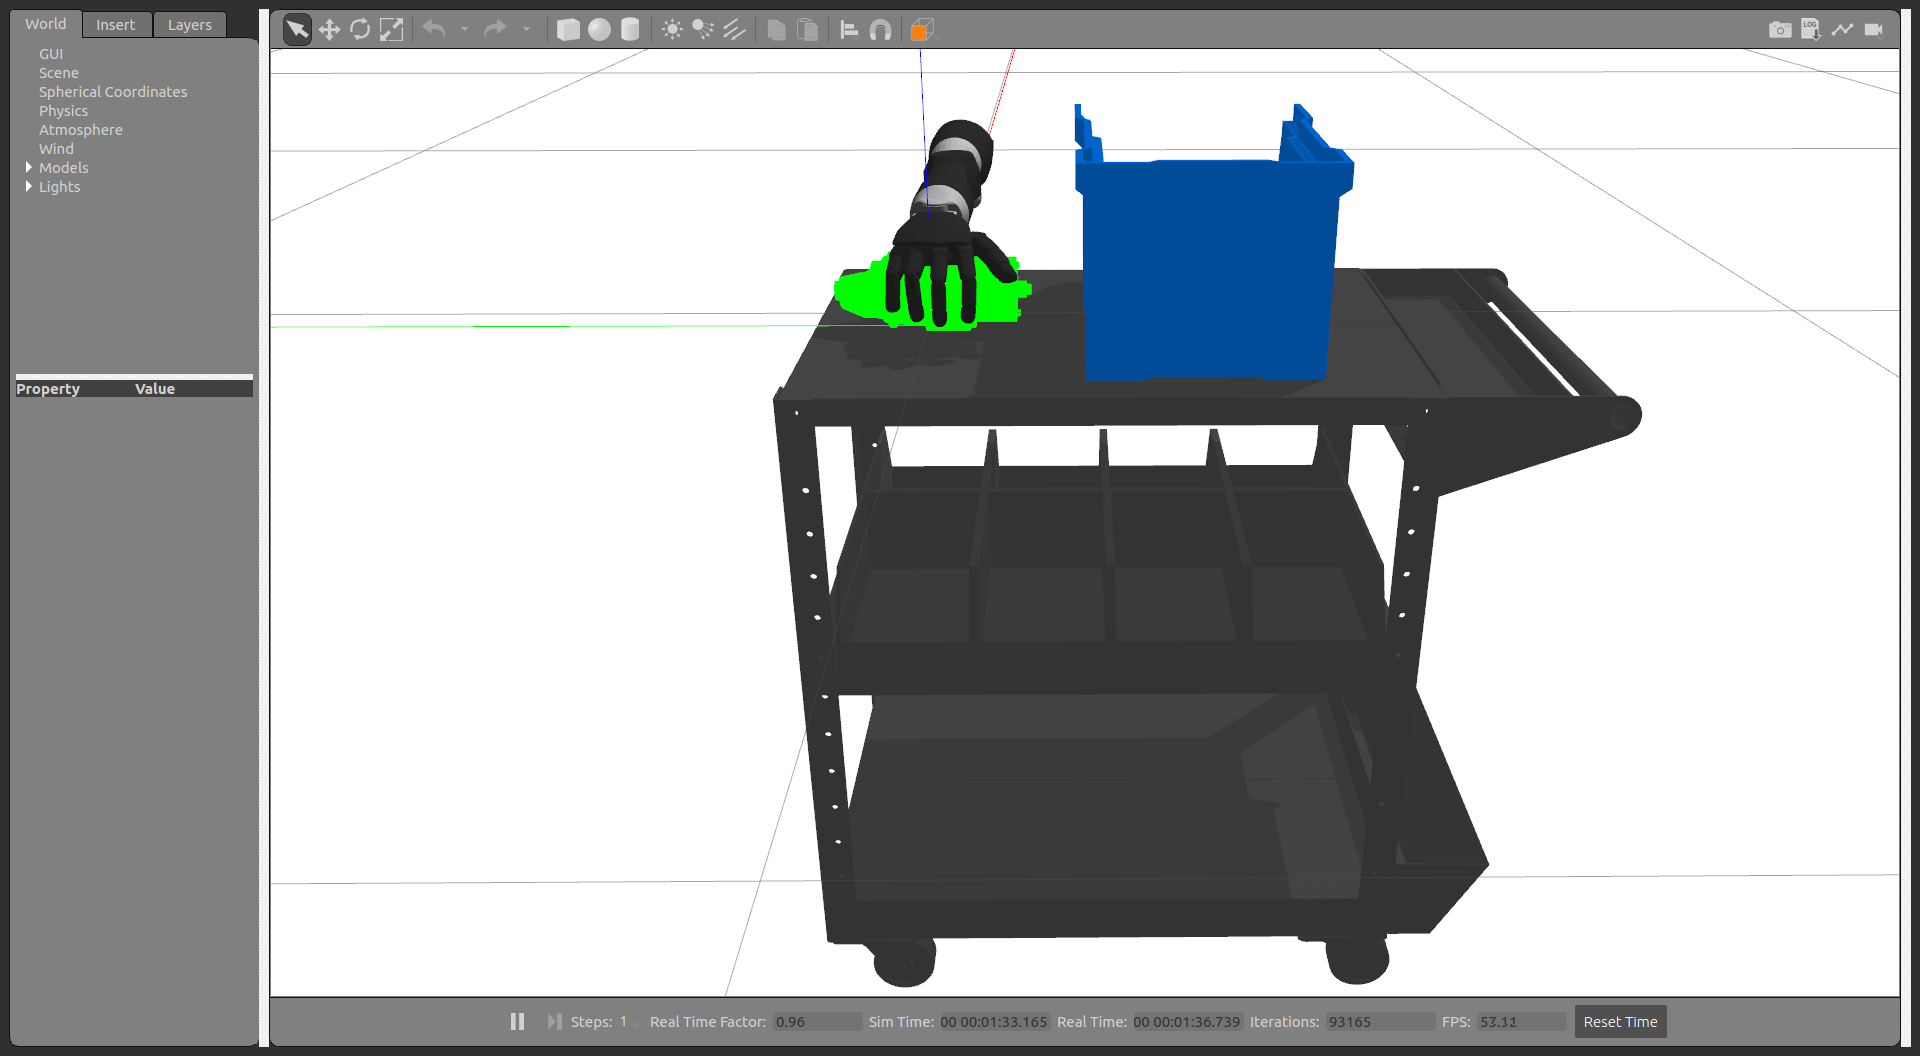
\includegraphics[width=.24\textwidth]{environments/active-perception/gazebo-back}
%	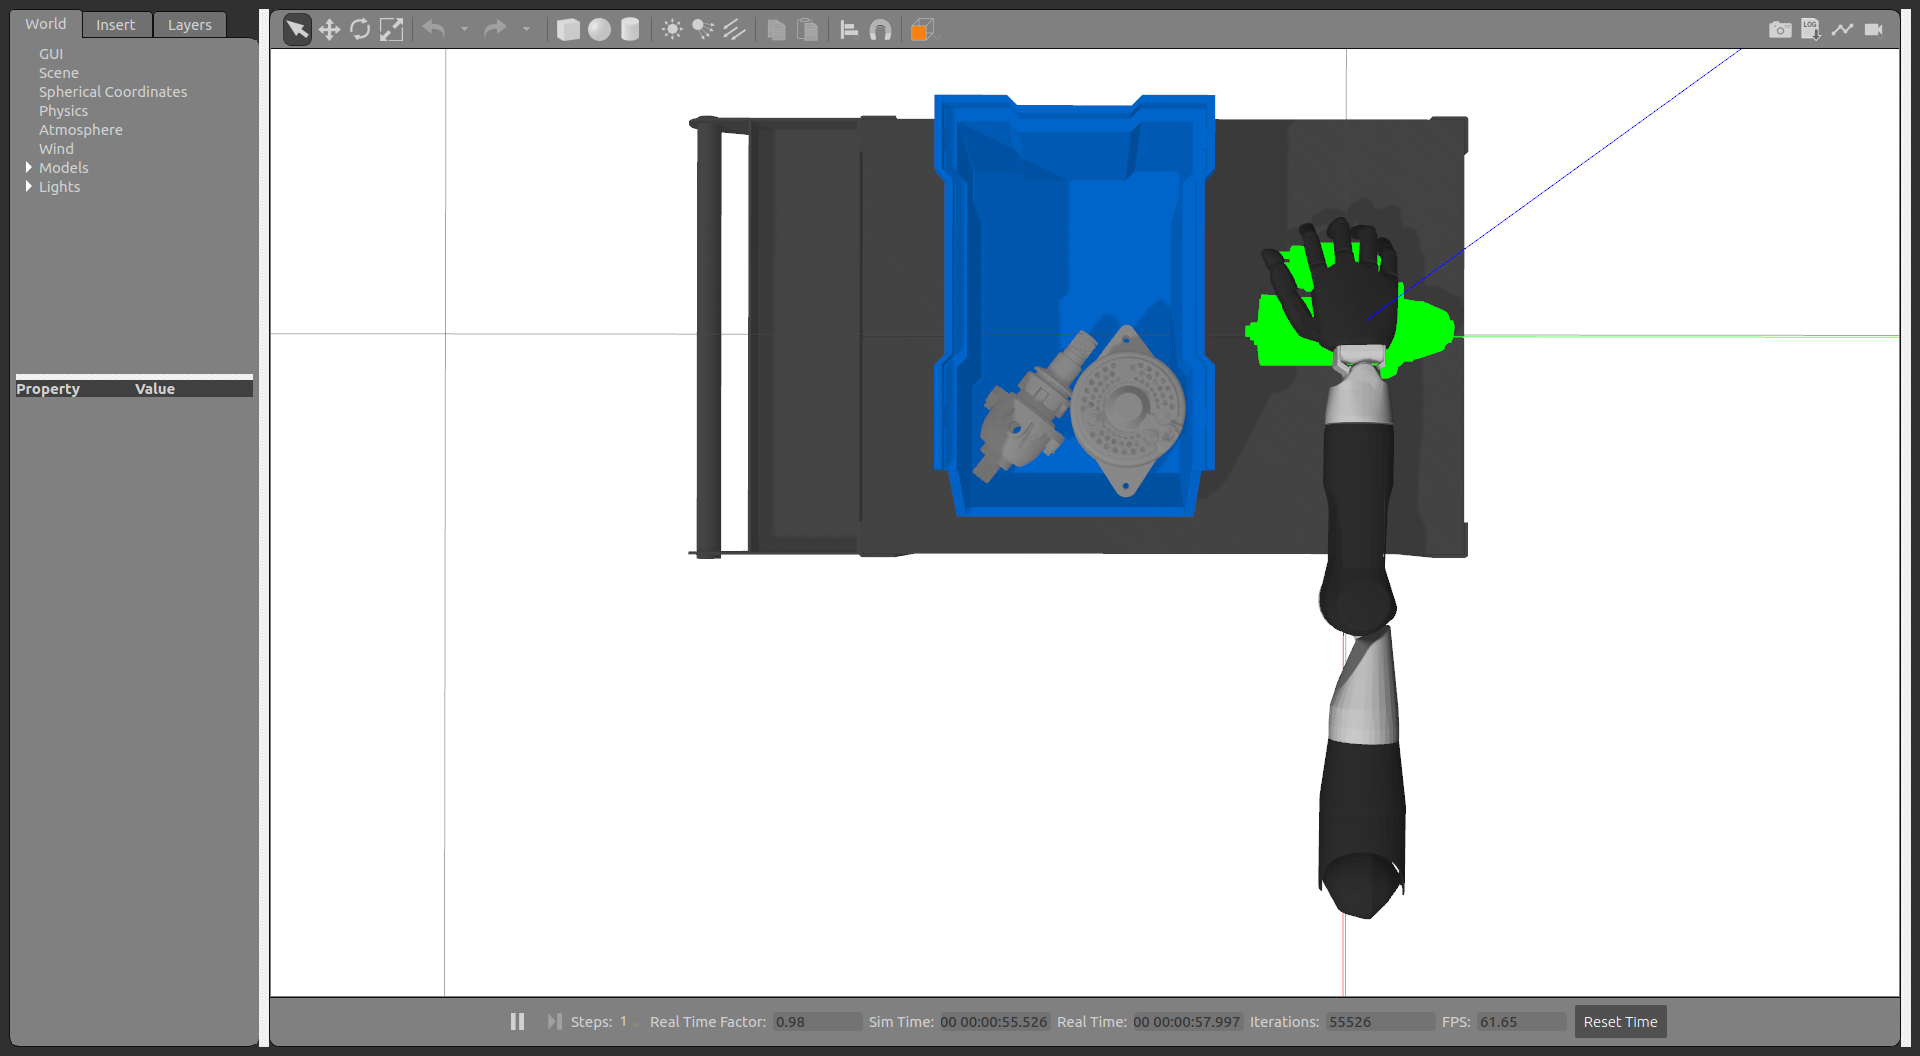
\includegraphics[width=.24\textwidth]{environments/active-perception/gazebo-top}
	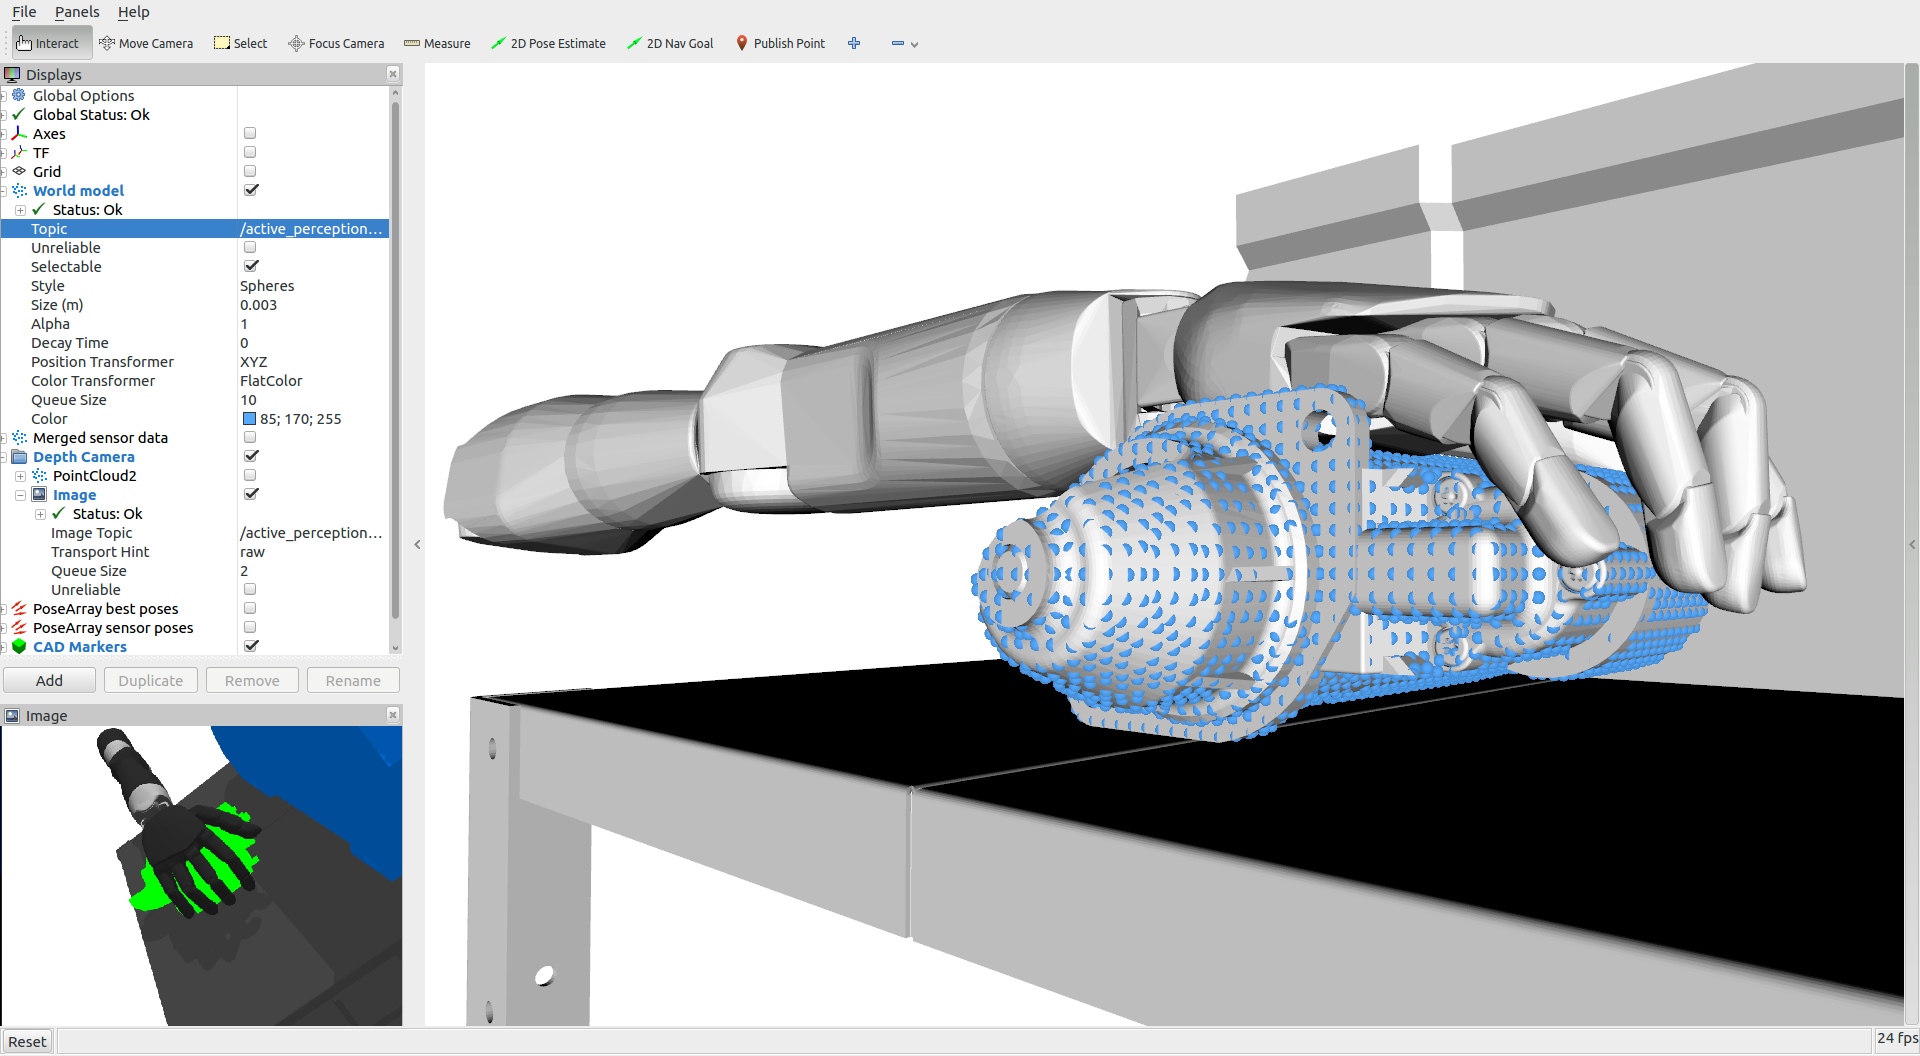
\includegraphics[width=.24\textwidth]{environments/active-perception/rviz-back-left}
%	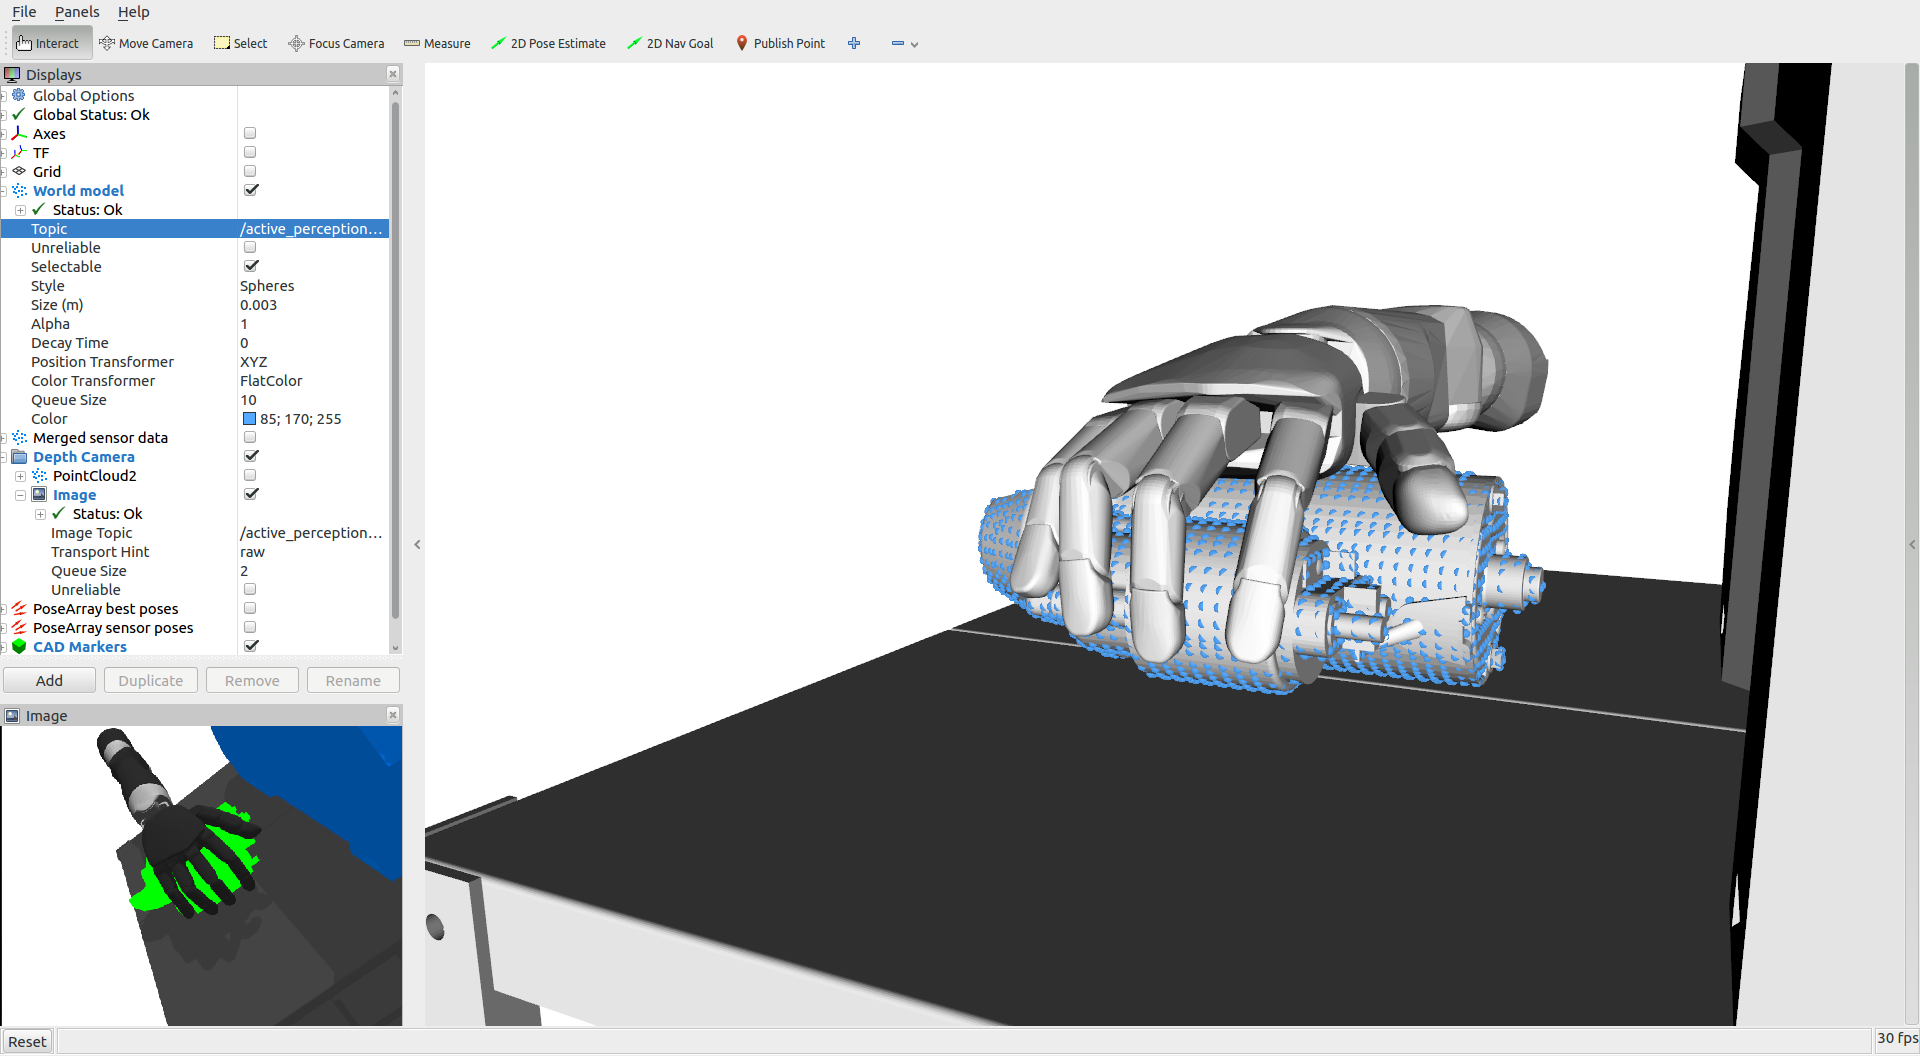
\includegraphics[width=.24\textwidth]{environments/active-perception/rviz-back-right}
	\caption{Environment for active perception of a starter motor being grasped by a human hand. The left image is showing a rendering from the Gazebo simulator with the target object in green color while the right image is displaying with blue spheres in Rviz the associated reference point cloud.}
	\label{fig:active-perception-environment}
\end{figure}

\begin{figure}[H]
	\centering
%	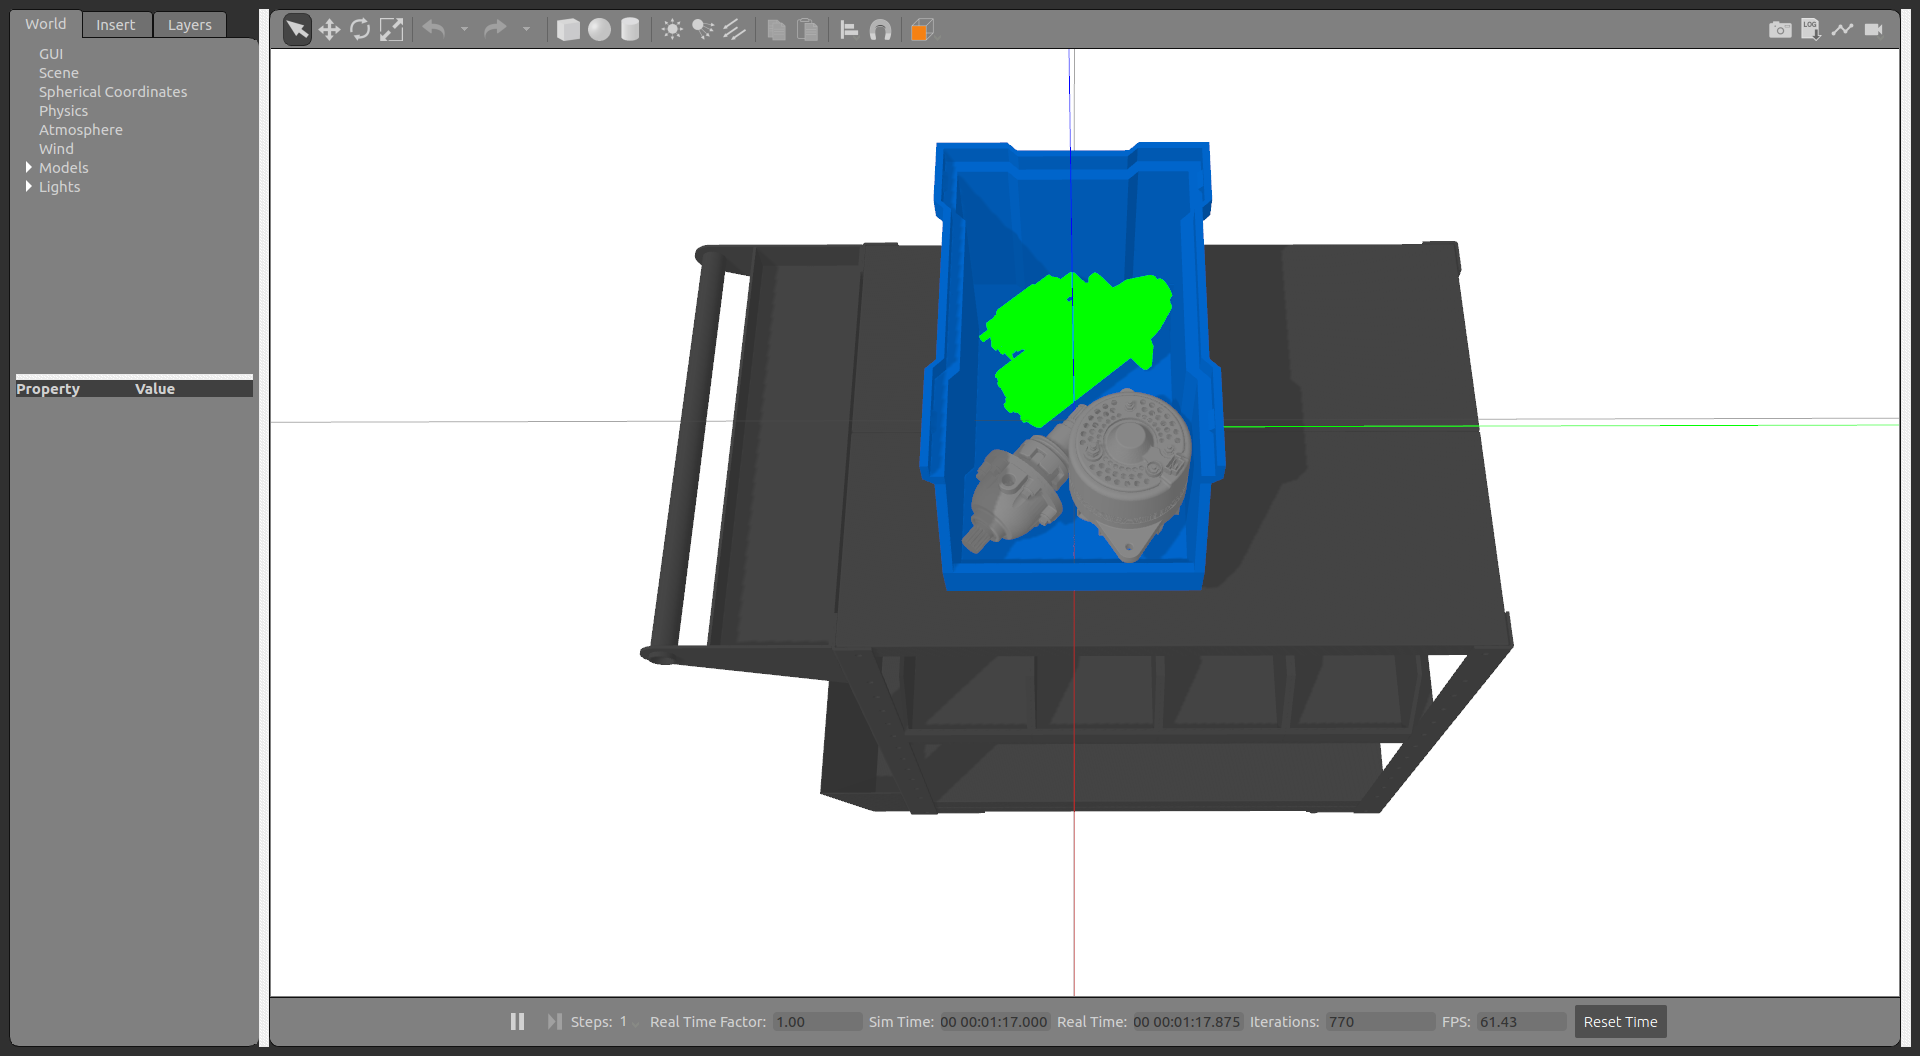
\includegraphics[width=.24\textwidth]{environments/bin-picking/gazebo-front}
	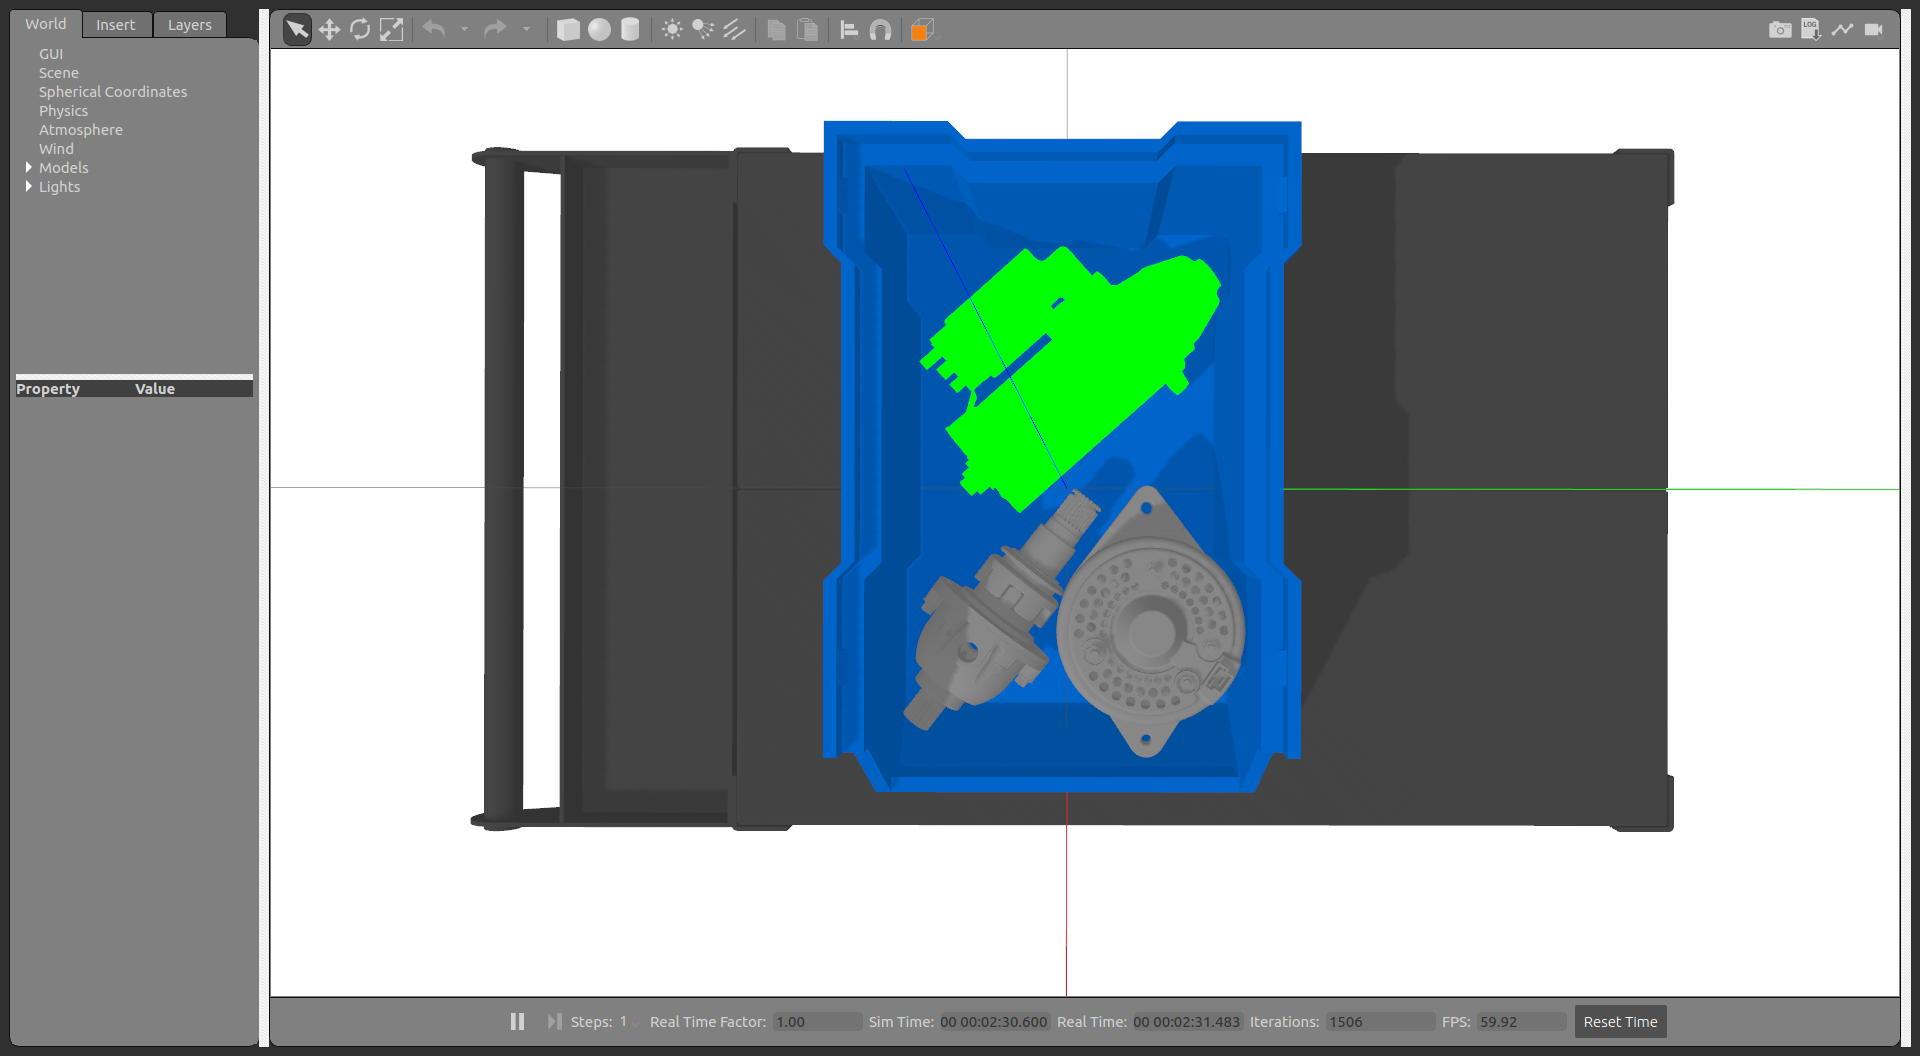
\includegraphics[width=.24\textwidth]{environments/bin-picking/gazebo-top}
%	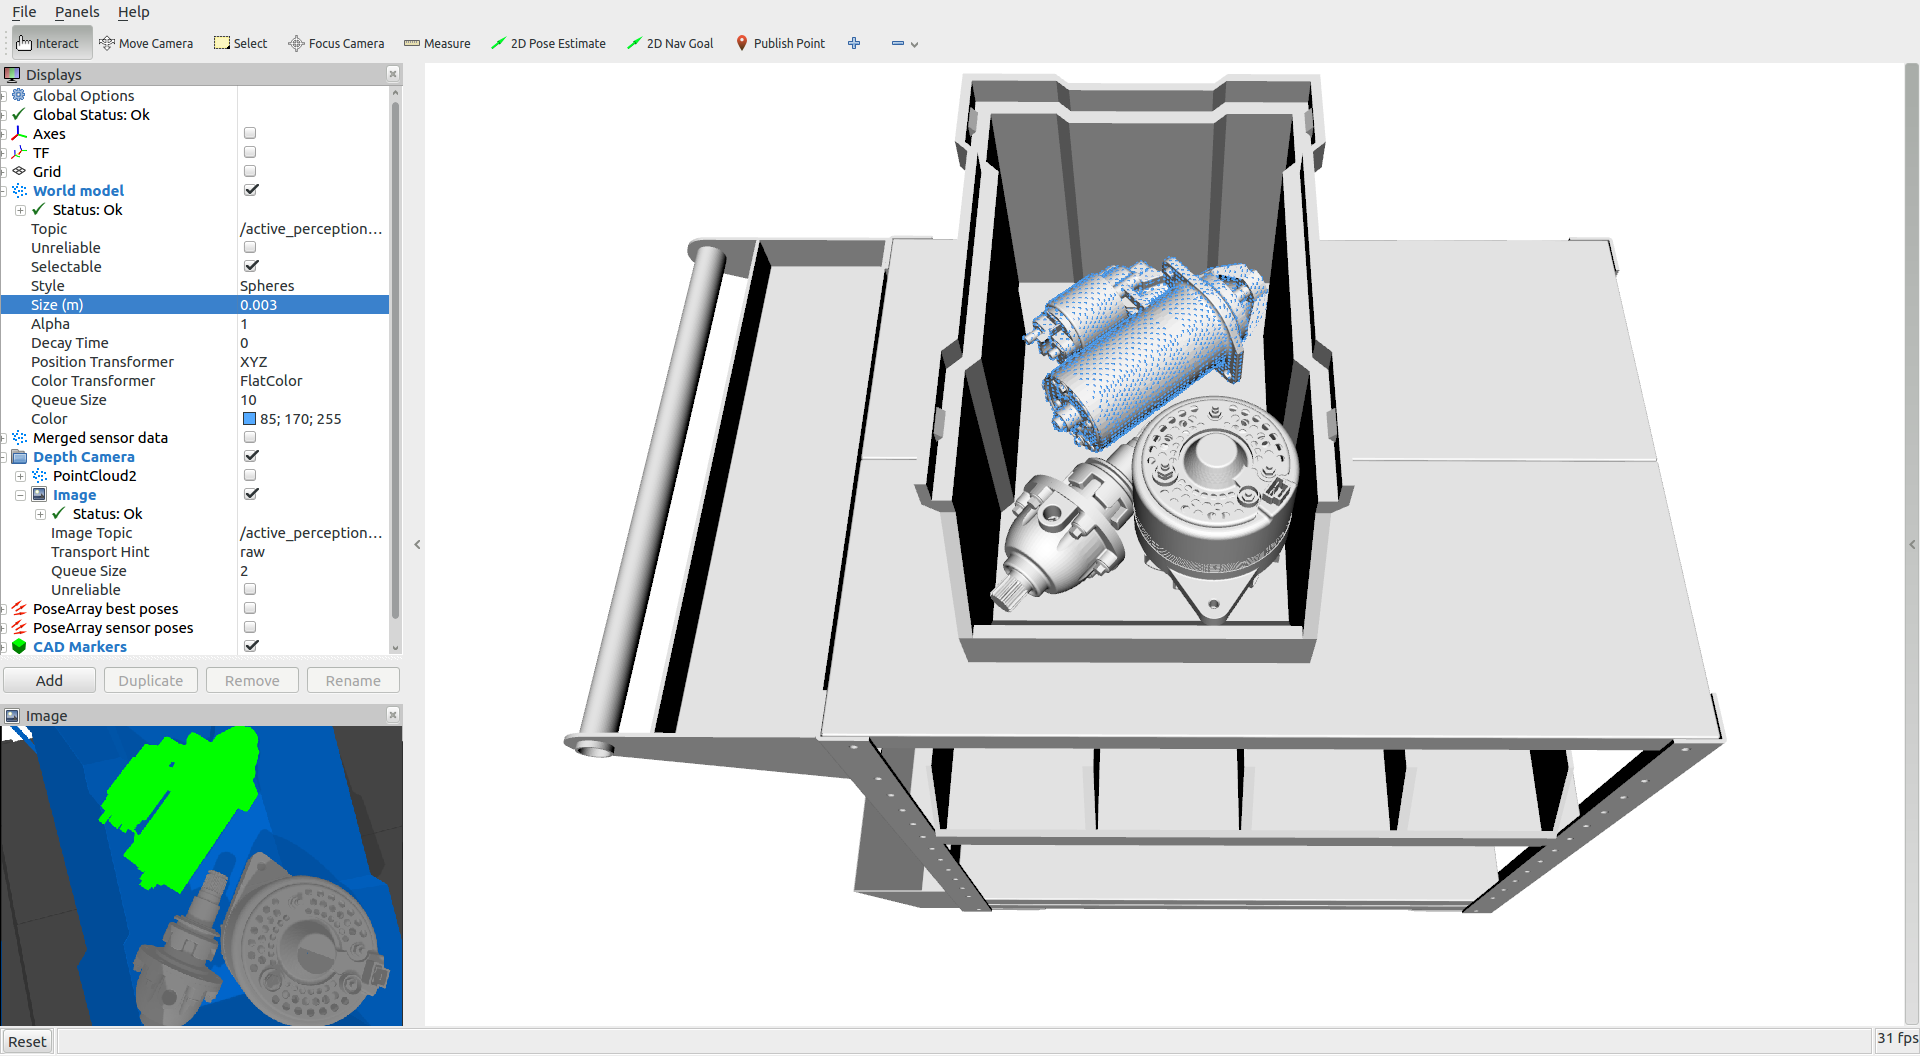
\includegraphics[width=.24\textwidth]{environments/bin-picking/rviz-front}
	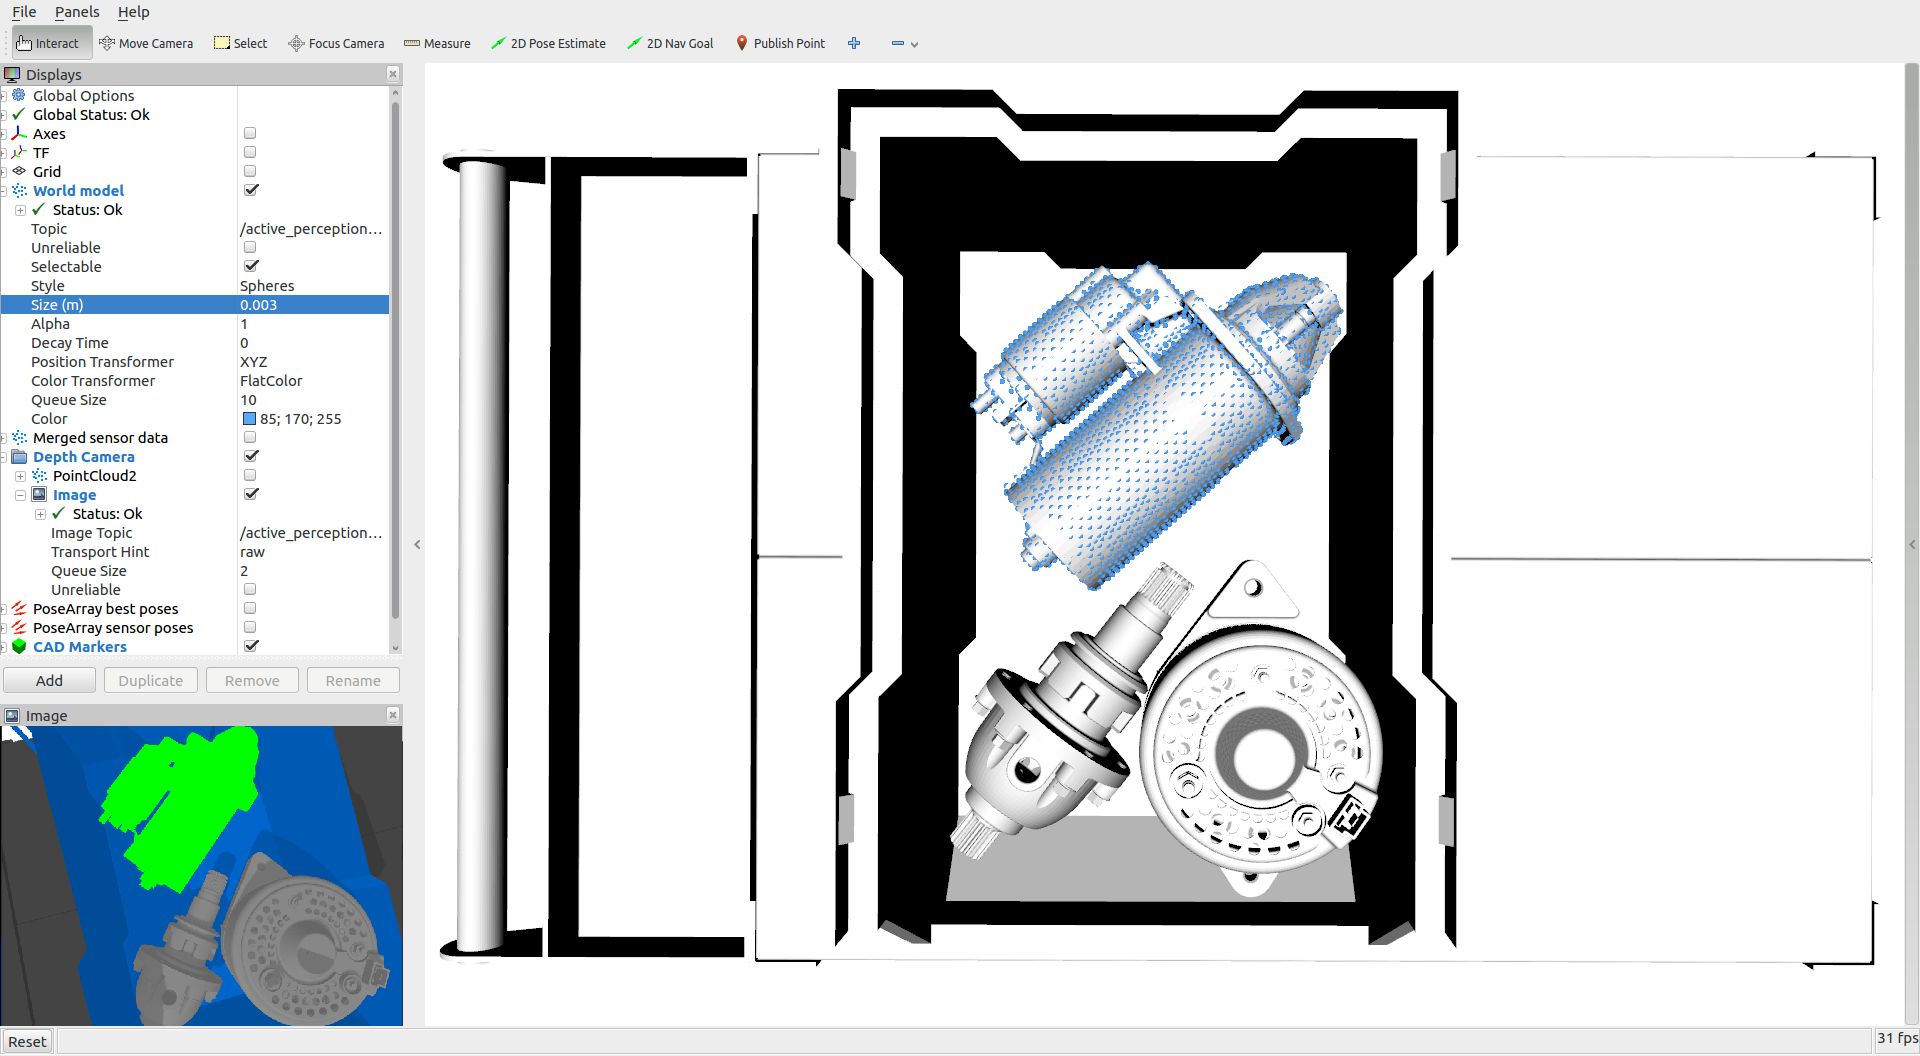
\includegraphics[width=.24\textwidth]{environments/bin-picking/rviz-top}
	\caption{Environment for bin picking of one starter motor that is inside a large staking box together with an alternator and a differential gearbox.}
	\label{fig:bin-picking-environment}
\end{figure}

\begin{figure}[H]
	\centering
%	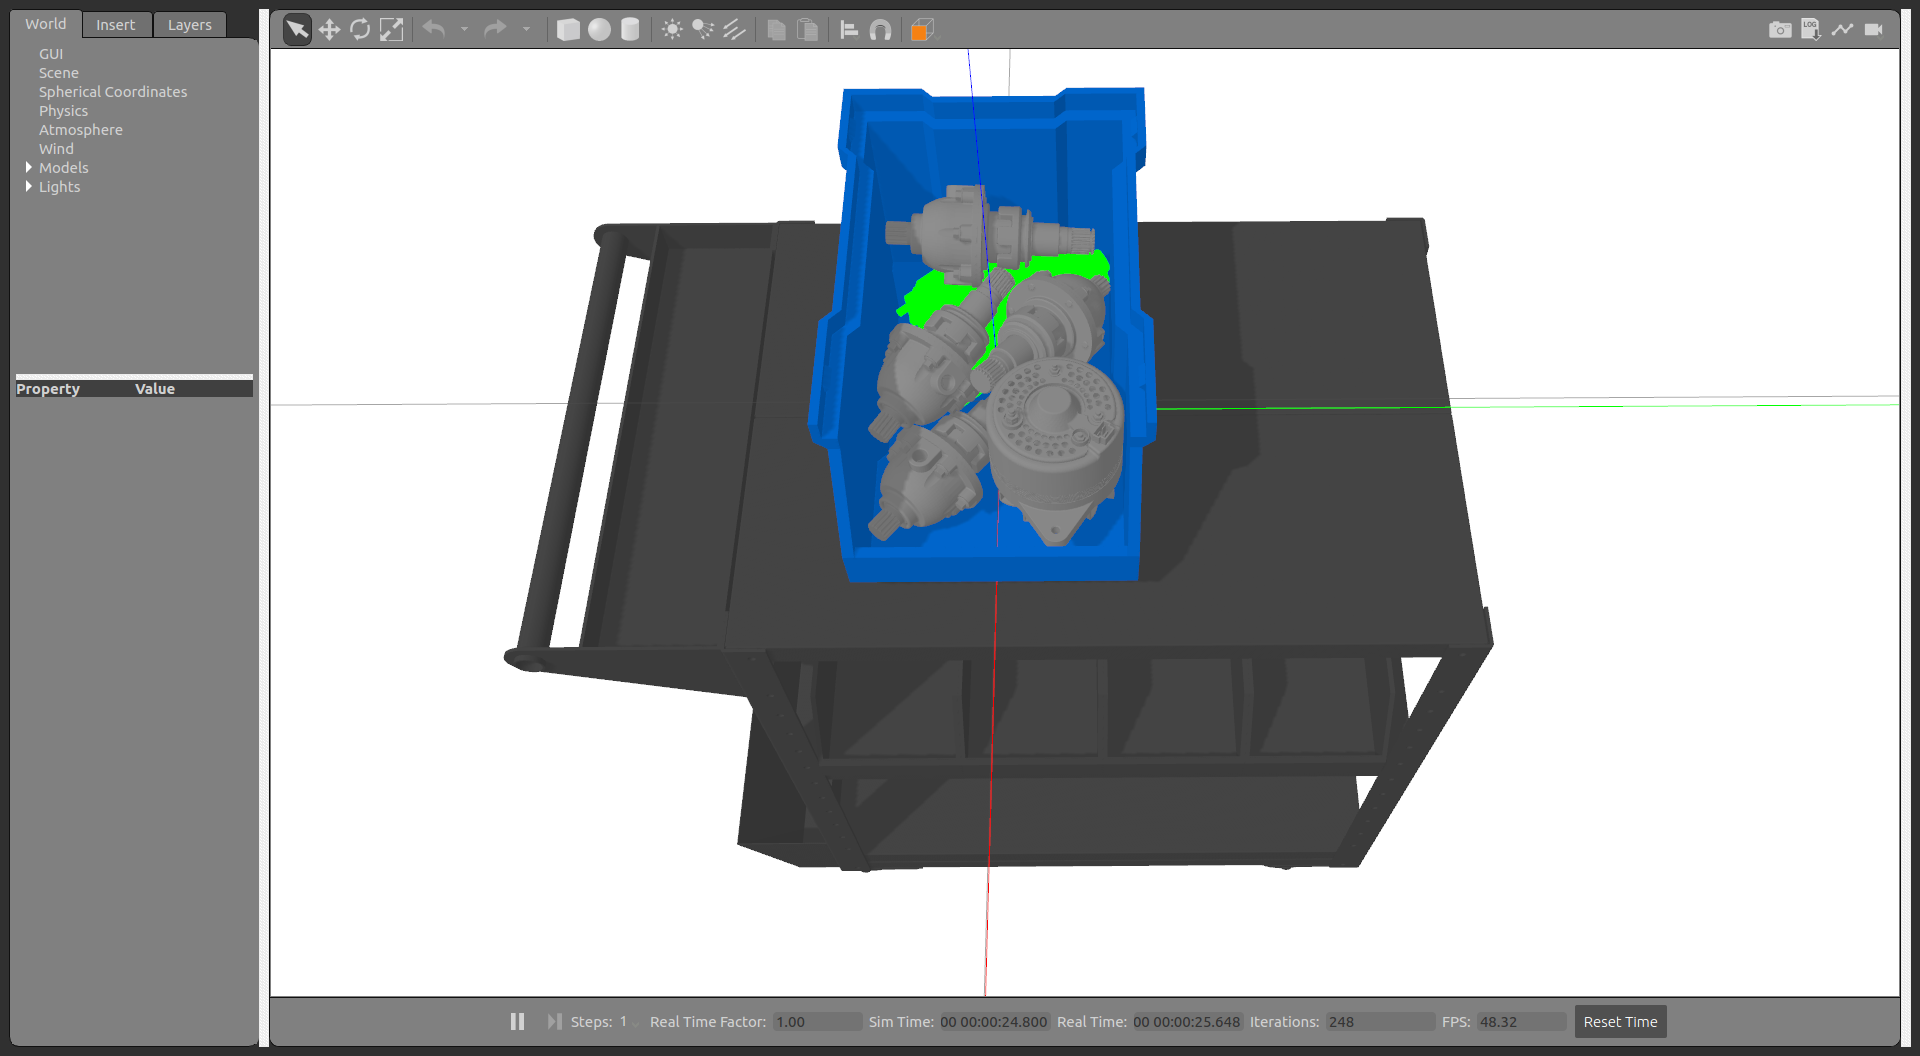
\includegraphics[width=.24\textwidth]{environments/bin-picking-with-occlusions/gazebo-front}
	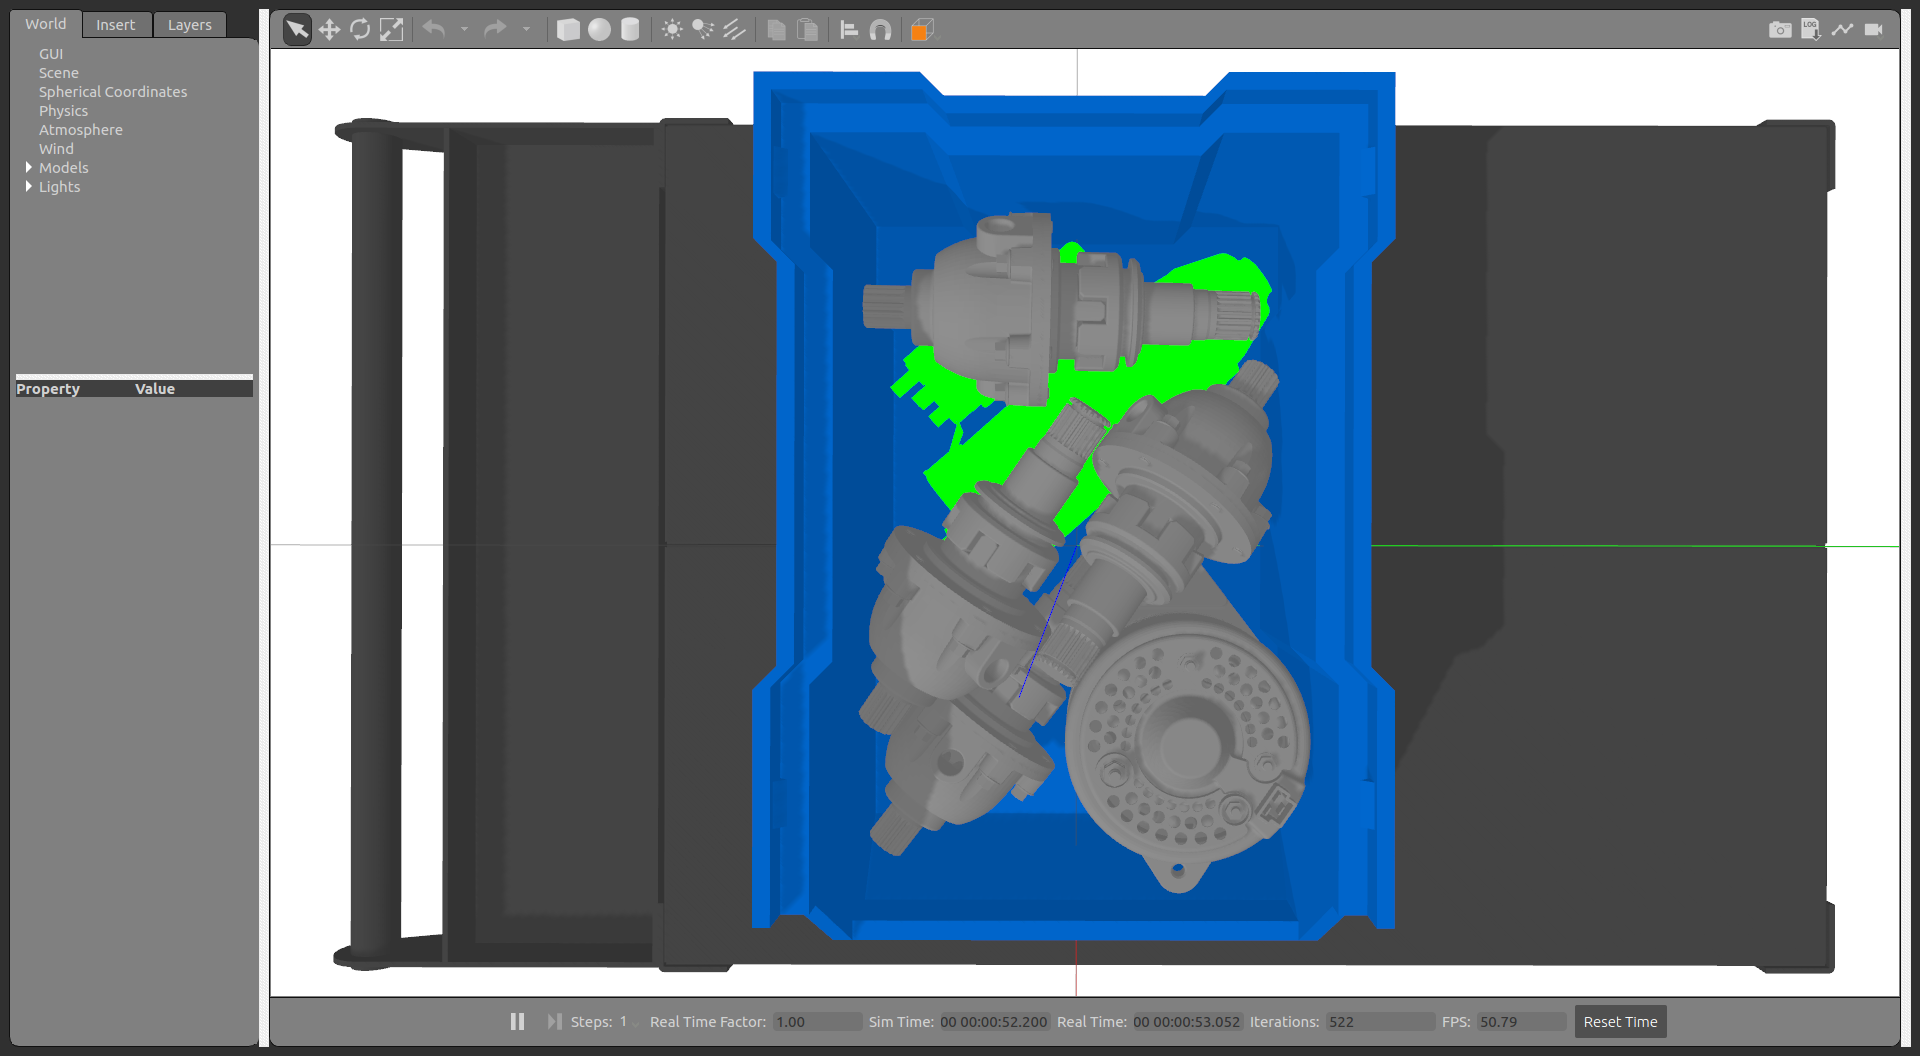
\includegraphics[width=.24\textwidth]{environments/bin-picking-with-occlusions/gazebo-top}
%	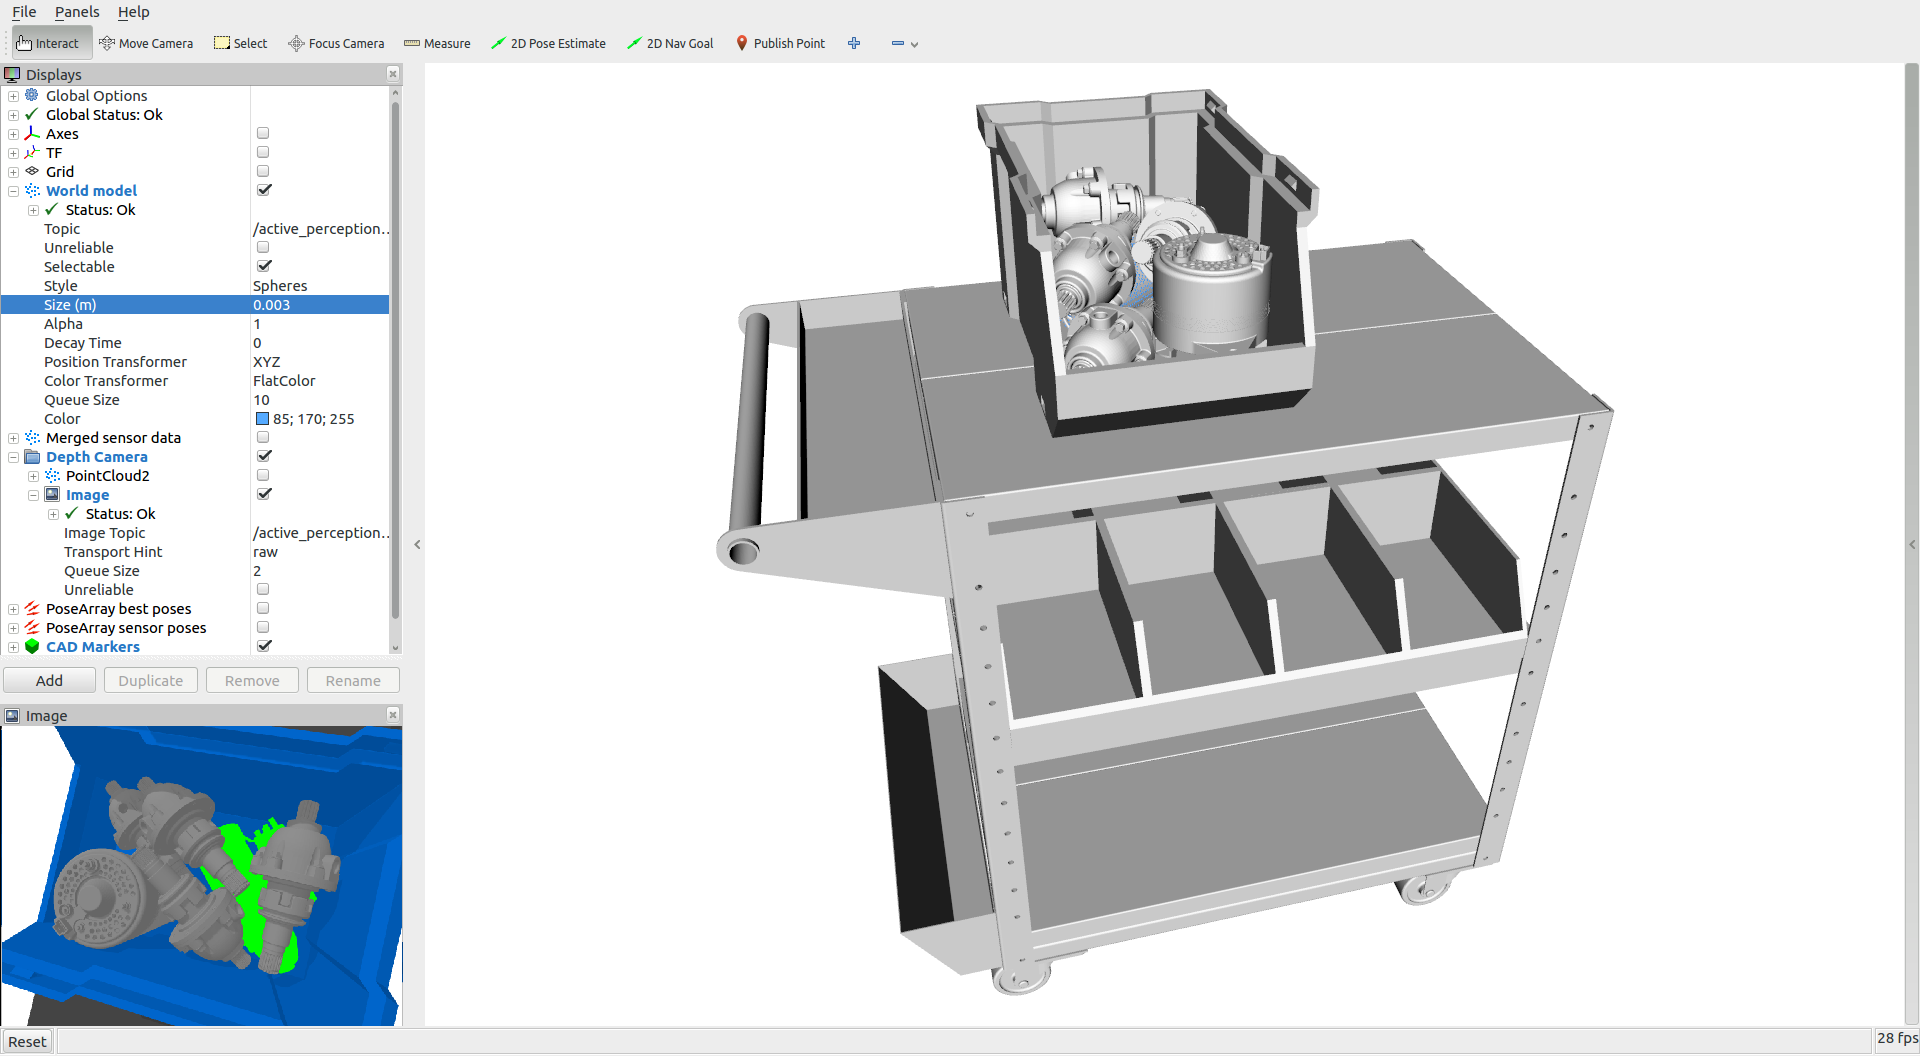
\includegraphics[width=.24\textwidth]{environments/bin-picking-with-occlusions/rviz-front}
	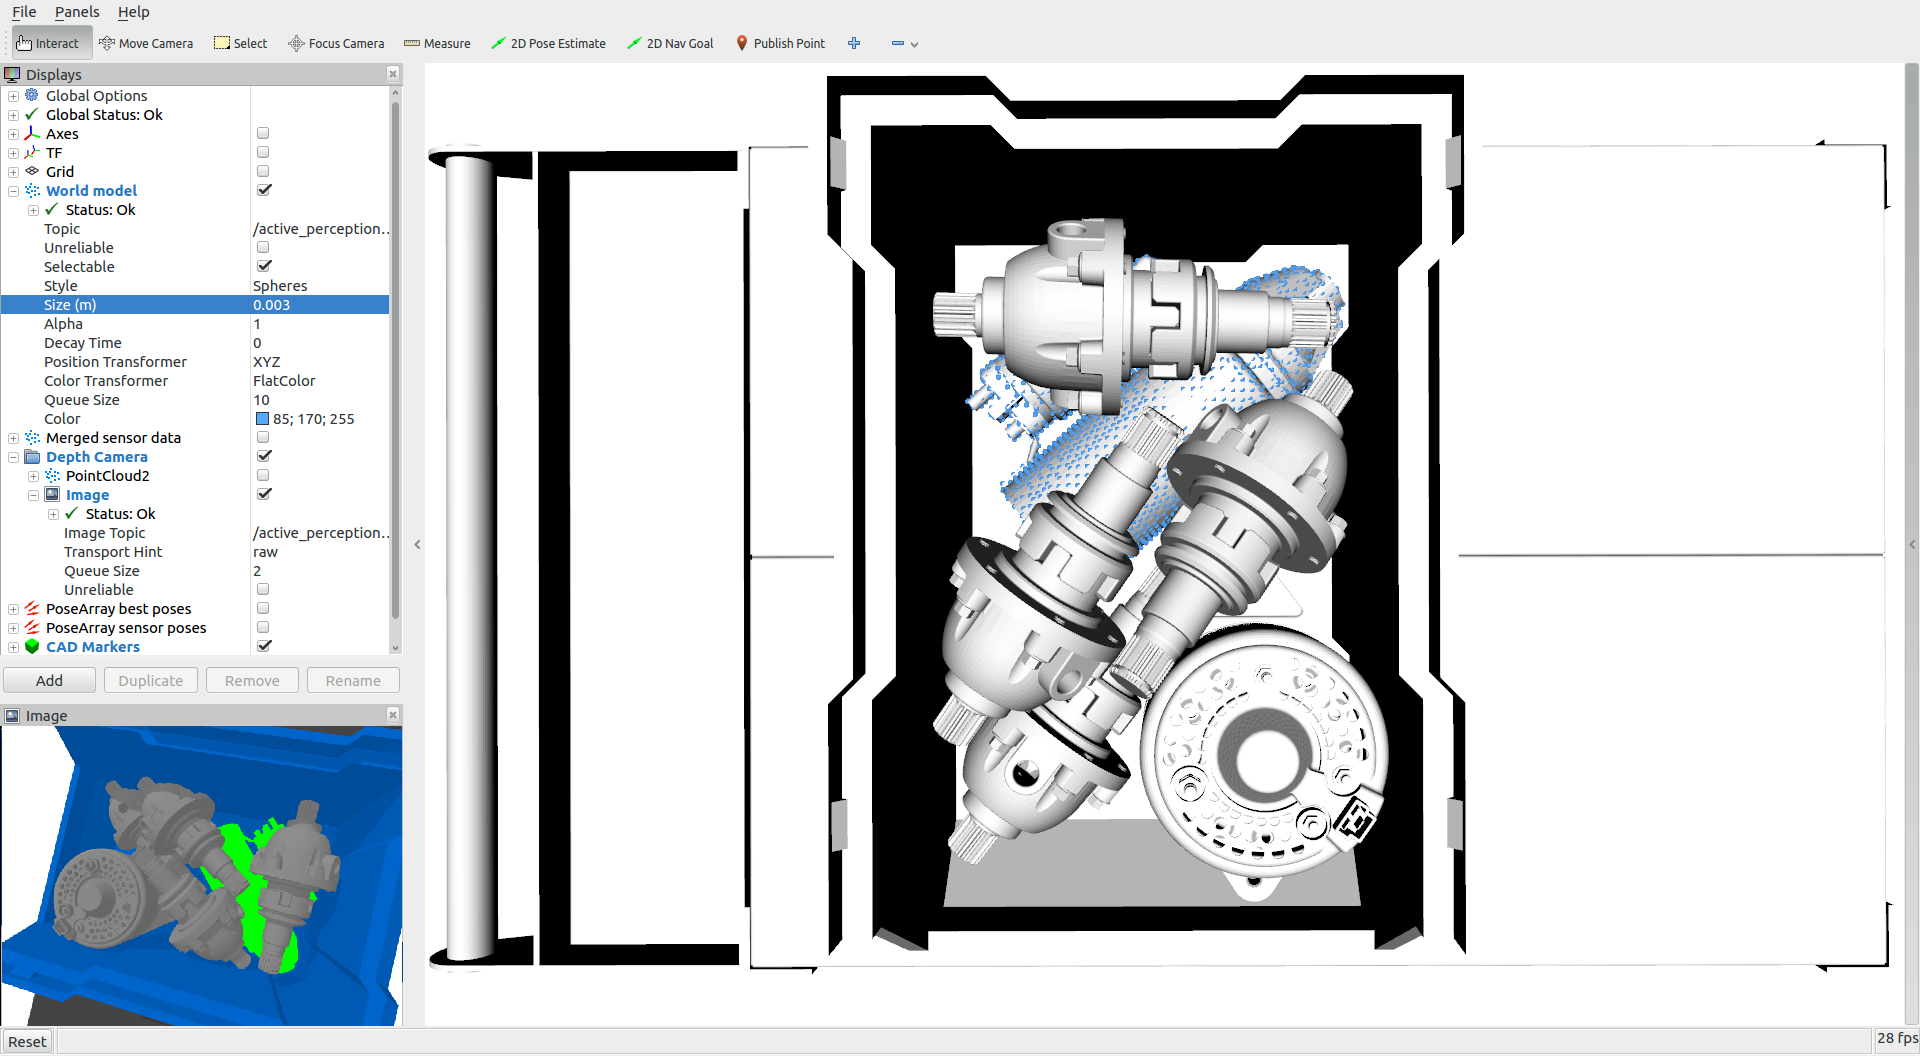
\includegraphics[width=.24\textwidth]{environments/bin-picking-with-occlusions/rviz-top}
	\caption{Environment for bin picking of one starter motor with 3 differential gearboxes causing occlusions.}
	\label{fig:bin-picking-with-occlusions-environment}
\end{figure}

\begin{figure}[H]
	\centering
	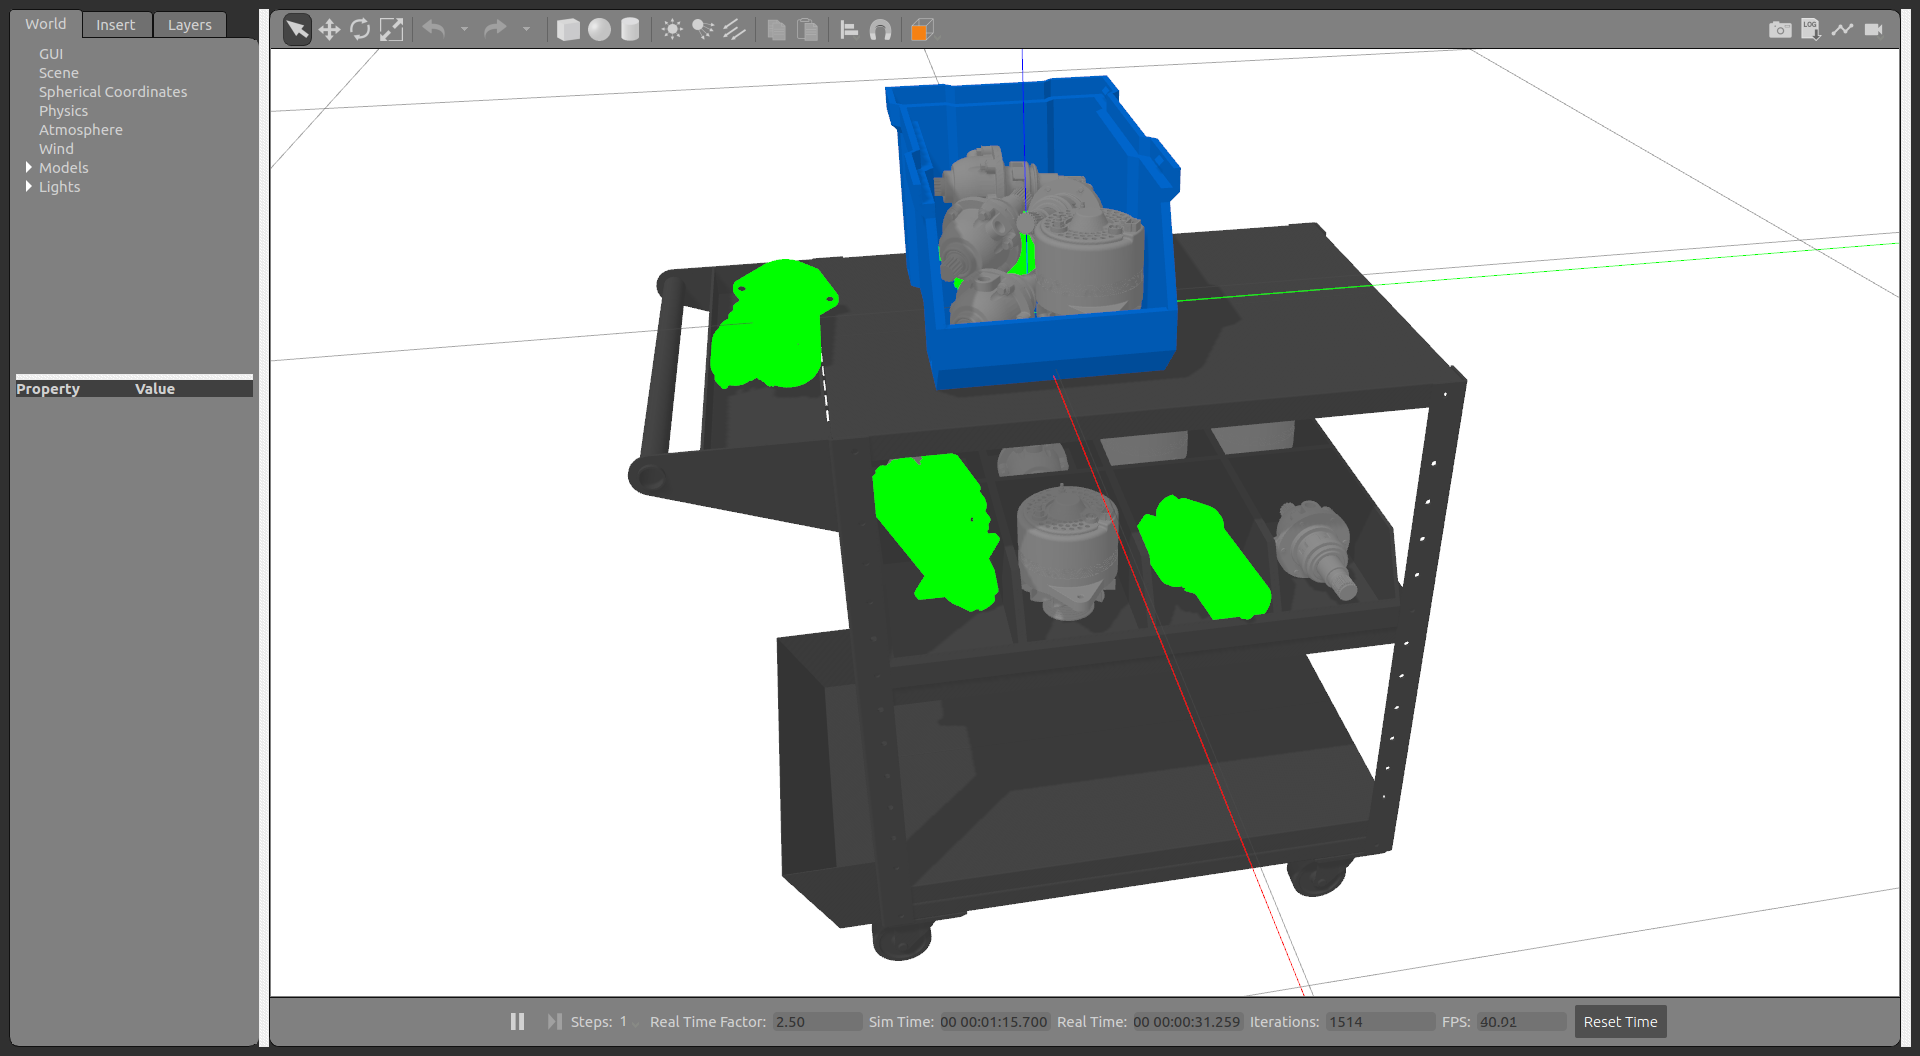
\includegraphics[width=.24\textwidth]{environments/multiple-bin-picking-with-occlusions/gazebo-front}
	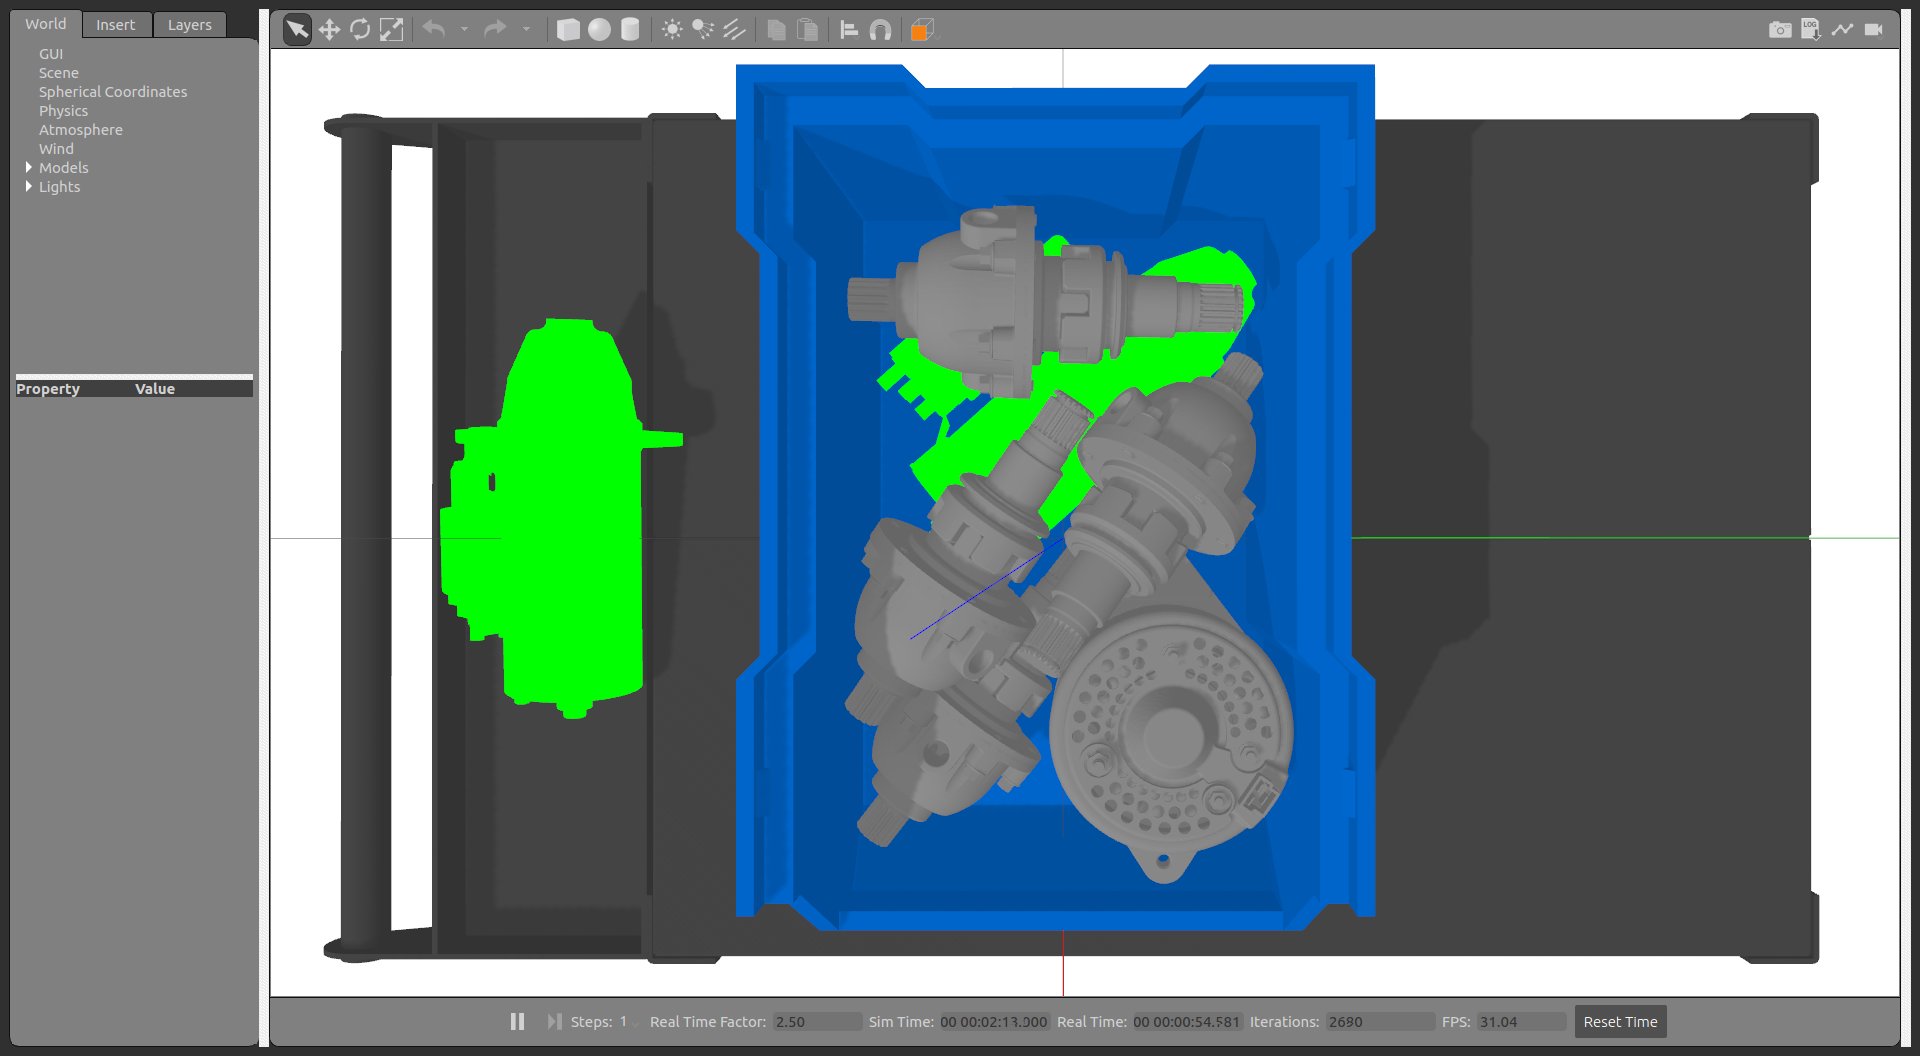
\includegraphics[width=.24\textwidth]{environments/multiple-bin-picking-with-occlusions/gazebo-top}\\
	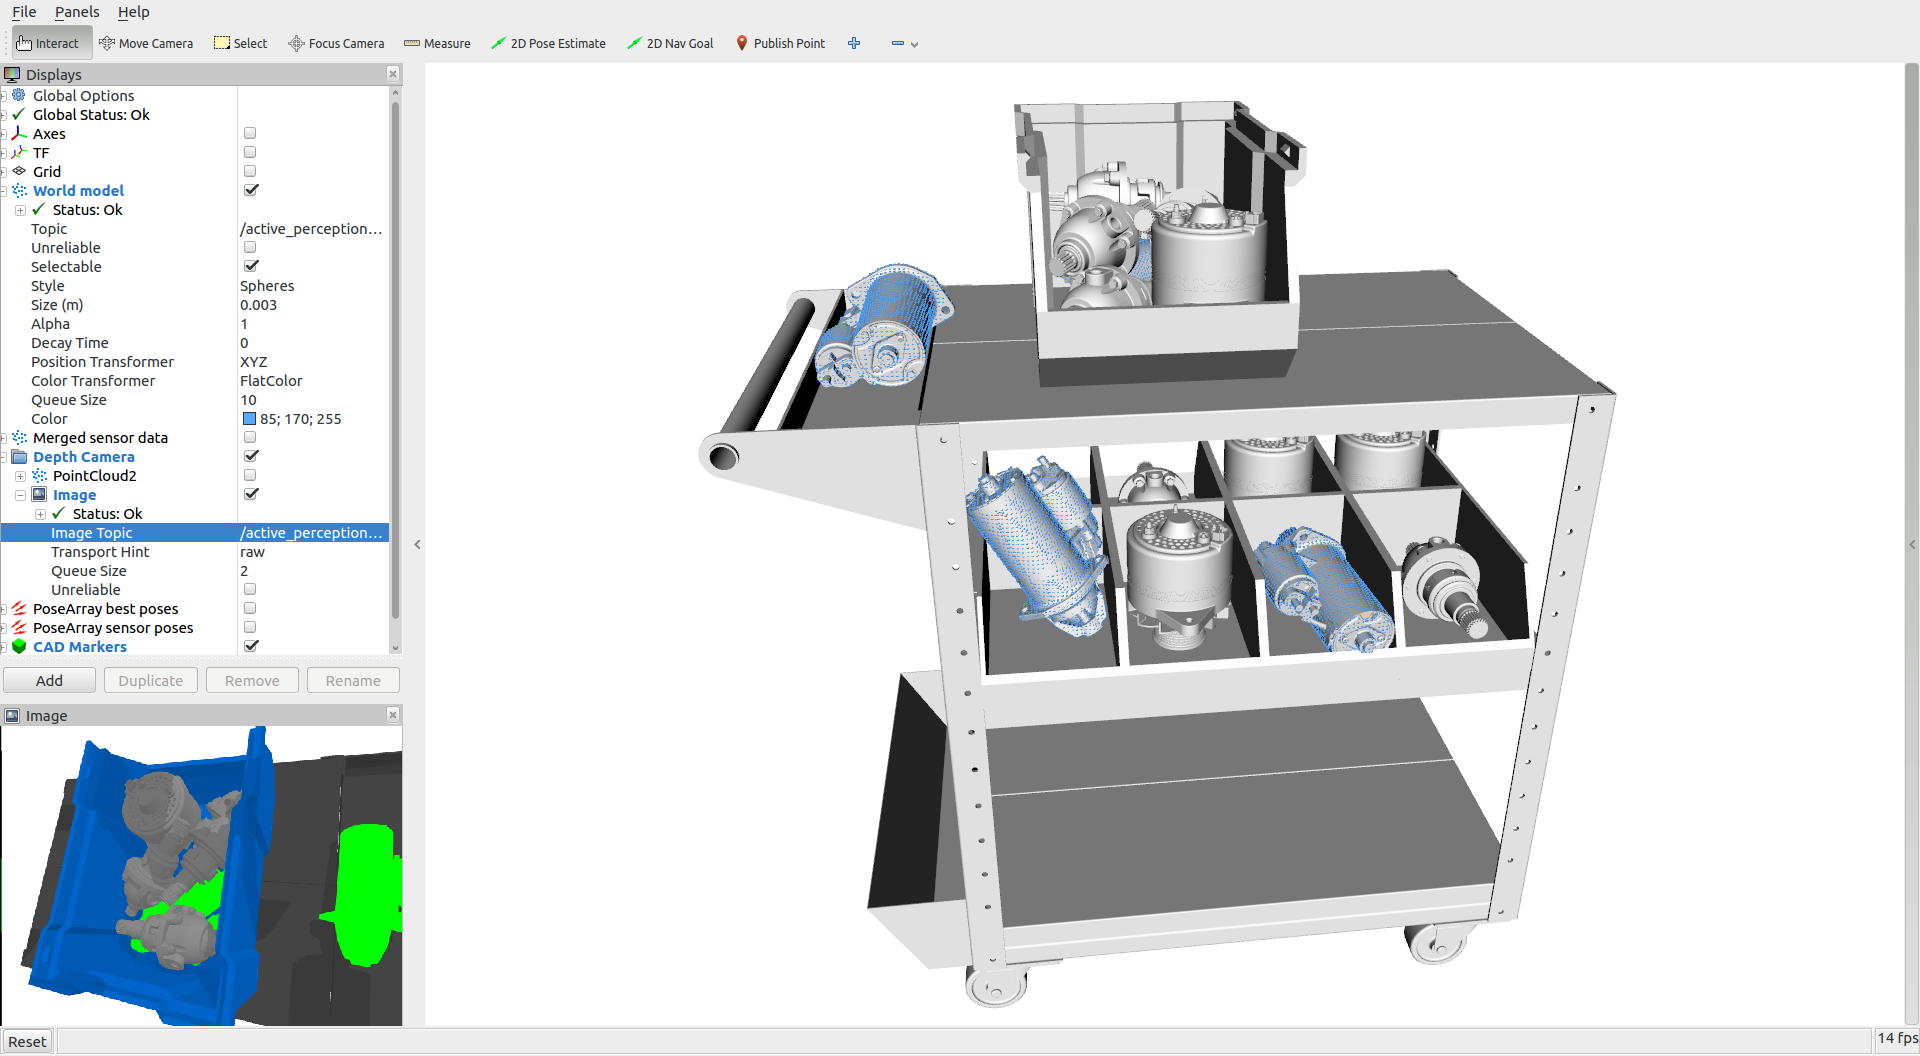
\includegraphics[width=.24\textwidth]{environments/multiple-bin-picking-with-occlusions/rviz-front-corner}
	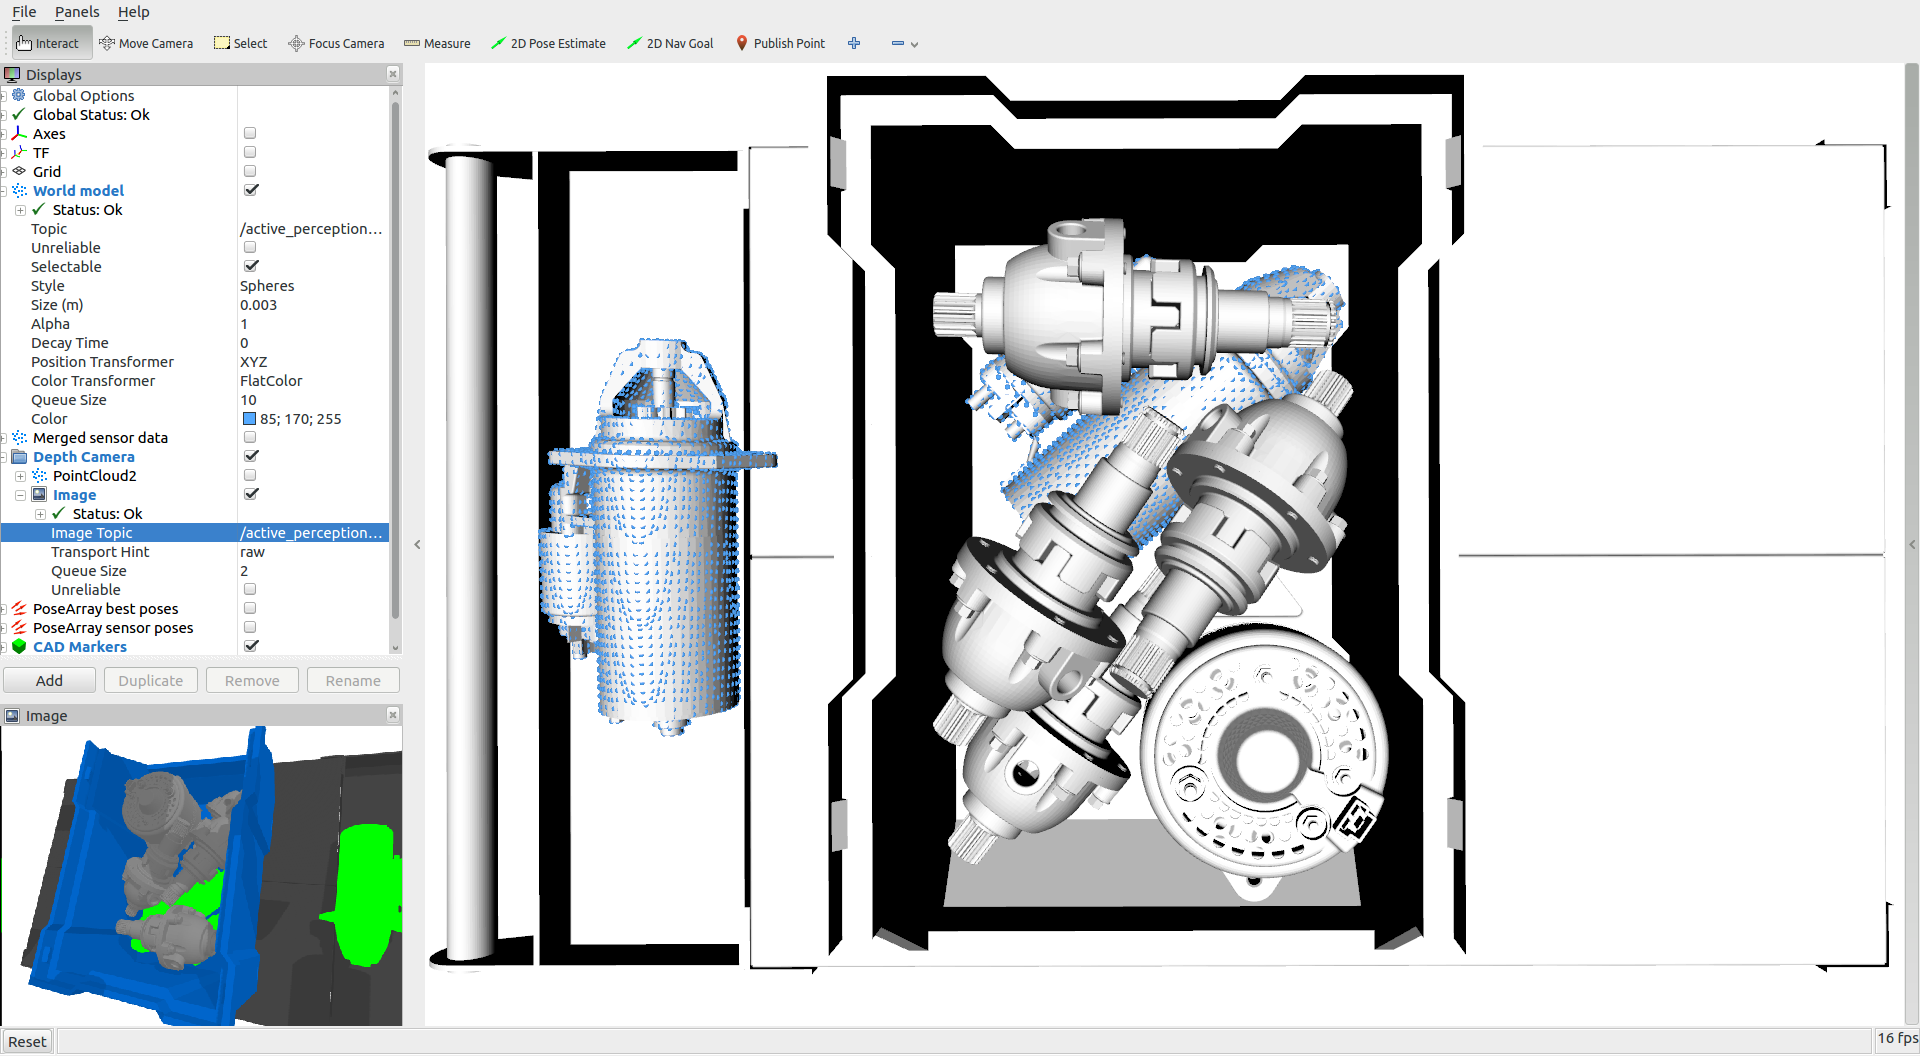
\includegraphics[width=.24\textwidth]{environments/multiple-bin-picking-with-occlusions/rviz-top}
	\caption{Environment for picking 4 starter motors with multiple occlusions.}
	\label{fig:multiple-bin-picking-with-occlusions-environment}
\end{figure}


\subsection{Sensors modeling}

Over the years it was developed a wide range of technologies for performing environment sensing. From the passive image sensors to the active systems that probe the environment using projected patterns, lasers or \gls{tof} devices. Given that the goal of the proposed system was to perform active perception or environment monitoring, it was modeled 8 different types of depth sensors (shown in \cref{fig:sensors}) which relied on 3 types of environment sensing technologies. One of them was the Kinect XBox One \gls{tof} device, 5 were structured light sensors (such as the Asus Xtion Pro Live, the Ensenso N35, the Intel RealSense SR300, the Kinect XBox 360 and the Orbbec Astra) and 2 were stereo vision systems (namely the MultiSense S7 and the ZED stereo camera). Each of these depth sensors can be modeled using the pinhole camera model, which allows to specify the main unique characteristics of each sensor, such as the depth image resolution (width and height in pixels), its \gls{fov} (horizontal and vertical in radians) and the range in which the sensor can retrieve valid measurements (minimum and maximum in meters). Moreover, since this camera model is implemented in most 3D rendering engines and optimized in todays powerful \glspl{gpu}, the sensor data generation can be performed very fast and efficiently using 3D rendering \glspl{api} such as the \gls{opengl}. This is the case of the Gazebo simulator, that uses the Ogre3D\footnote{\url{http://www.ogre3d.org}} rendering engine which in turn relies on \gls{opengl}. Besides camera modeling, Gazebo also allows to simulate the sensor acquisition rate (specified as the number of depth images generated per second), which is usually higher on structured light sensors and lower on stereo vision systems.

\begin{figure}
	\centering
	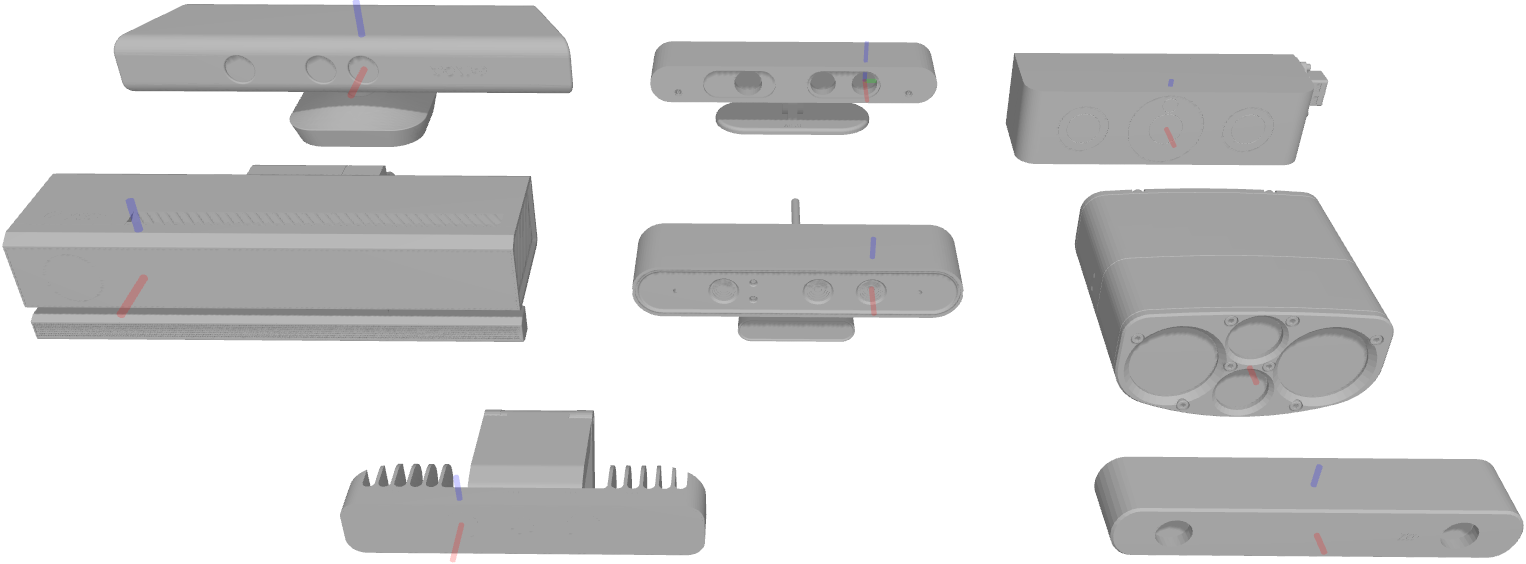
\includegraphics[width=.47\textwidth]{sensors/sensors-gray-with-links}
	\caption{CAD models of the 3D sensors with the display of the depth image coordinate frames using the ROS convention of x-y-z -> forward-left-up. Name of the 3D sensors from top left to bottom right: Kinect XBox 360, Asus Xtion Pro Live, Ensenso N35, Kinect XBox One, Orbbec Astra, MultiSense S7, Intel RealSense SR300, ZED stereo camera.}
	\label{fig:sensors}
\end{figure}


\subsection{Sensors deployment}\label{subsec:sensors-deployment}

Finding the optimal sensor constellation that maximizes the observed surface area of a given set of target objects is a challenging combinatorial explosive problem when considering the presence of occlusions within the environment. As such, for making the estimation of the sensor disposition computational feasible, the 3D continuous space was populated with a given set of sensors within regions of interest while looking at a specified observation point (with the sensor roll either 0º or random). This approach allows to reduce the sensor pose estimation from a 6 \gls{dof} to a 4 \gls{dof} problem (x, y, z position plus the sensor rotation along the observation axis). Moreover, the continuous solution space with an infinite amount of observation view points is reduced to a bounded number in which the sensors can either be deployed uniformly or randomly inside regions of interest. This allows to sample the solution space with a reasonable and representative amount of simulated sensor data for computing a good enough sensor disposition for the problem at hand.

The proposed system allows the deployment of several populations of sensors within a simulated world. Each population contains a given number of sensors of the same type that can be deployed uniformly / randomly within a box / cylinder or in a grid / linear disposition. This allows to deploy the sensors in the simulated environment spaces that represent valid positions for the real sensors. For example, limiting the possible sensor view points to the walls and ceiling of a room, avoiding deploying sensors in areas in which they could not provide any valuable sensor data or in which they could not be physically placed due to spatial restrictions or safety reasons.

The populations of sensors that were deployed on the 4 simulation worlds were fine tuned to the particular goals of each test. For the active perception environment, 450 sensors were deployed close to the target object, on the top, right and back side of the trolley (shown in \cref{fig:sensors-deployment-active-perception-environment}). This was done to simulate the closest range in which a dynamically moving sensor attached to a robotic arm could move (taking into consideration the human safety and the sensor minimum measurement distance, that was 0.2 meters).

\begin{figure}[H]
	\centering
	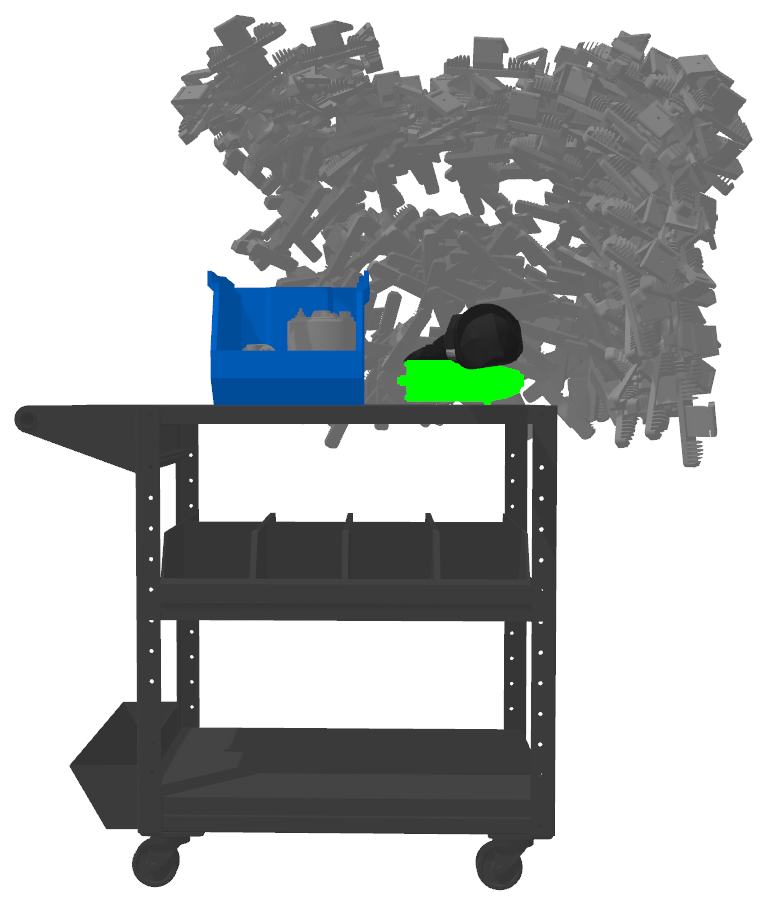
\includegraphics[height=.22\textwidth]{sensor-deployment/active-perception/gazebo-front}\hspace{1em}
	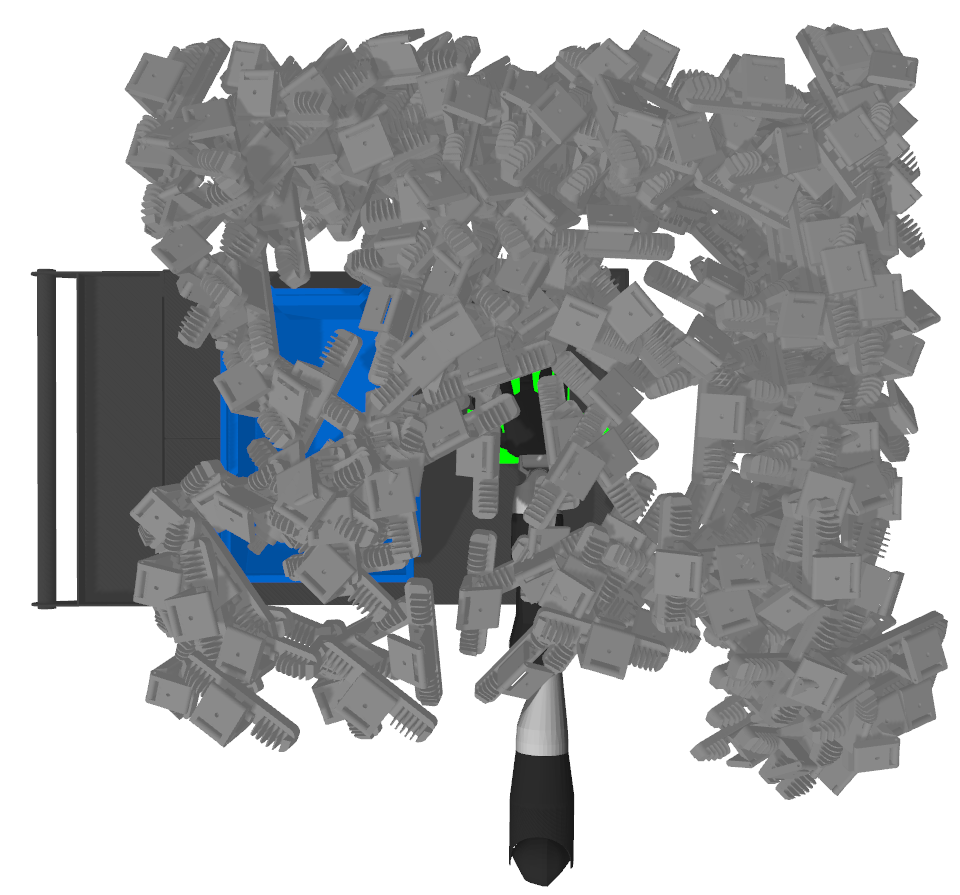
\includegraphics[height=.22\textwidth]{sensor-deployment/active-perception/gazebo-top}
	\caption{Sensors deployment for the active perception environment.}
	\label{fig:sensors-deployment-active-perception-environment}
\end{figure}

For the single object bin picking environments, given that the target object was inside the stacking box, the sensors were deployed close to the target object (displayed in \cref{fig:sensors-deployment-bin-picking-environments}), but only on top of the trolley, on 3 layers (each with a different type of sensor). In the world with minimal occlusions it were deployed 100 sensors while in the world with significant occlusions it were deployed 300 sensors. The sensor density was increased because when there is a high amount of occlusions, the best views have tighter observation regions, which could be missed with a sparse sensor deployment.

For the multiple object bin picking environment, given that there were several target objects (1 inside the stacking box, 1 on top of the trolley and 2 on the shelves of the trolley), it were deployed 450 sensors across 7 populations (visualized in \cref{fig:sensors-deployment-multiple-bin-picking-environment}), 5 of them simulating fixed sensors on the walls and ceiling and 2 of them simulating dynamic sensors attached to a robotic arm above the trolley.

It should be noted that the visual sensor disposition shown in \cref{fig:sensors-deployment-active-perception-environment,fig:sensors-deployment-bin-picking-environments,fig:sensors-deployment-multiple-bin-picking-environment} was for human visual inspection only. During the sensor data generation, the 3D models of the sensors are hidden to avoid occlusion of the scene objects.

\begin{figure}[H]
	\centering
	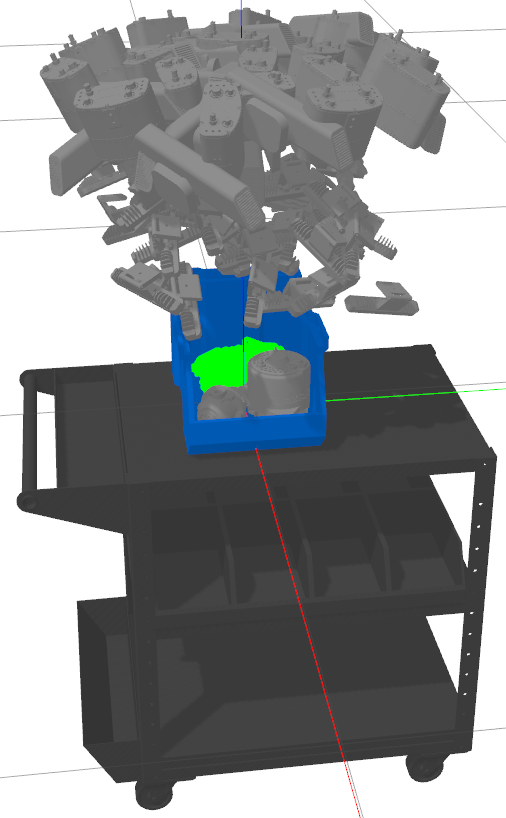
\includegraphics[height=.28\textwidth]{sensor-deployment/bin-picking/gazebo-sensors}\hspace{1em}
	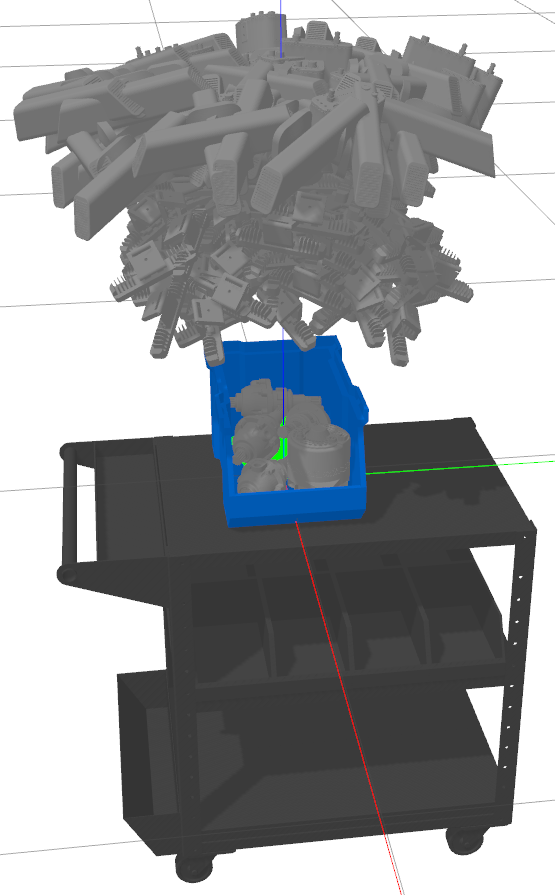
\includegraphics[height=.28\textwidth]{sensor-deployment/bin-picking-with-occlusions/gazebo-sensors}
	\caption{2 sensors deployments for the 1 object bin picking environments.}
	\label{fig:sensors-deployment-bin-picking-environments}
\end{figure}

\begin{figure}[H]
	\centering
	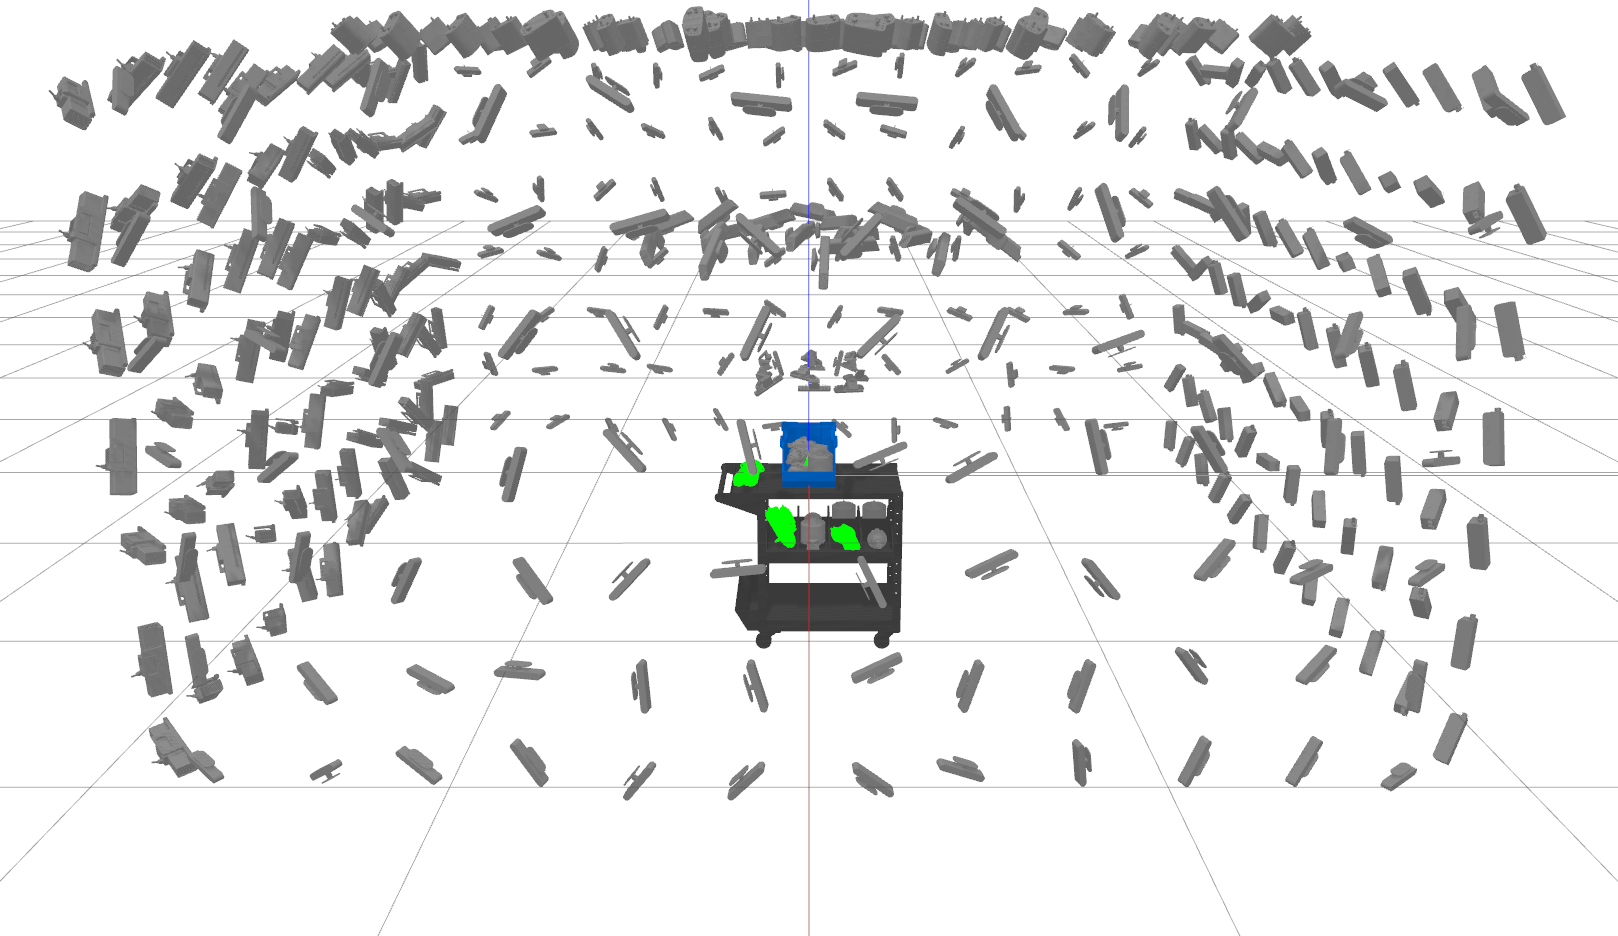
\includegraphics[height=.17\textwidth]{sensor-deployment/multiple-bin-picking-with-occlusions/gazebo-front}\hspace{0.25em}
	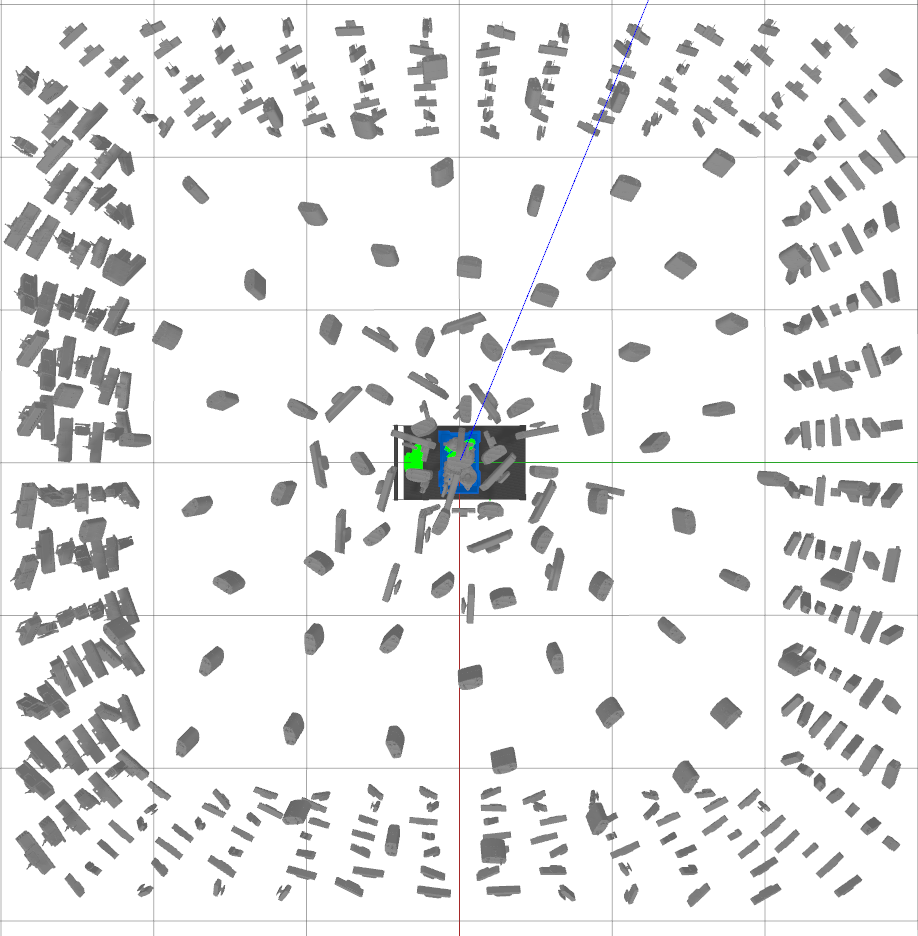
\includegraphics[height=.17\textwidth]{sensor-deployment/multiple-bin-picking-with-occlusions/gazebo-top}
	\caption{Sensors deployment for the multiple object bin picking environment.}
	\label{fig:sensors-deployment-multiple-bin-picking-environment}
\end{figure}

\section{\uppercase{Best views estimation}}\label{sec:best-views-estimation}

\noindent Implementation text.

\subsection{Reference surface point cloud}

\begin{itemize}
	\item The first step in the processing pipeline includes the generation of the multi-object reference point cloud that is assembled using the CAD data and the objects poses given by the simulator, which is later on filtered with a voxel grid algorithm to perform a regular spatial partition and extract the points that are in the surface voxels centroids
\end{itemize}
\begin{figure}
	\centering
	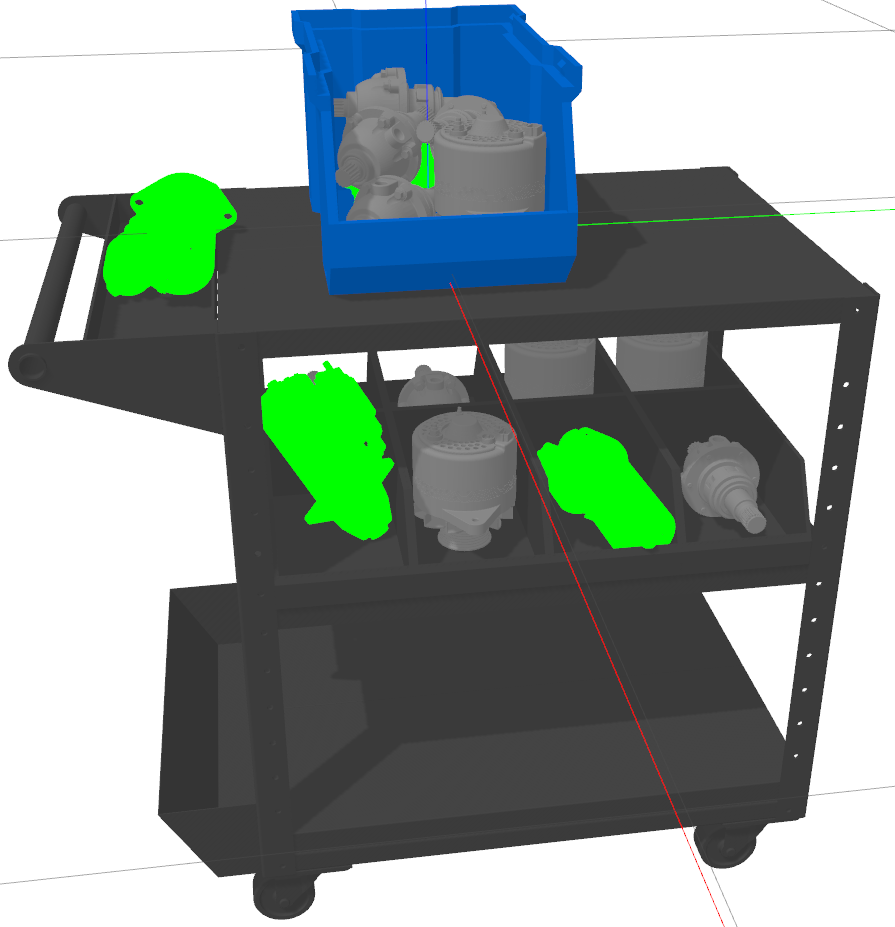
\includegraphics[height=.14\textheight]{sensor-data-processing/multimodel-environment}\hspace{2em}
	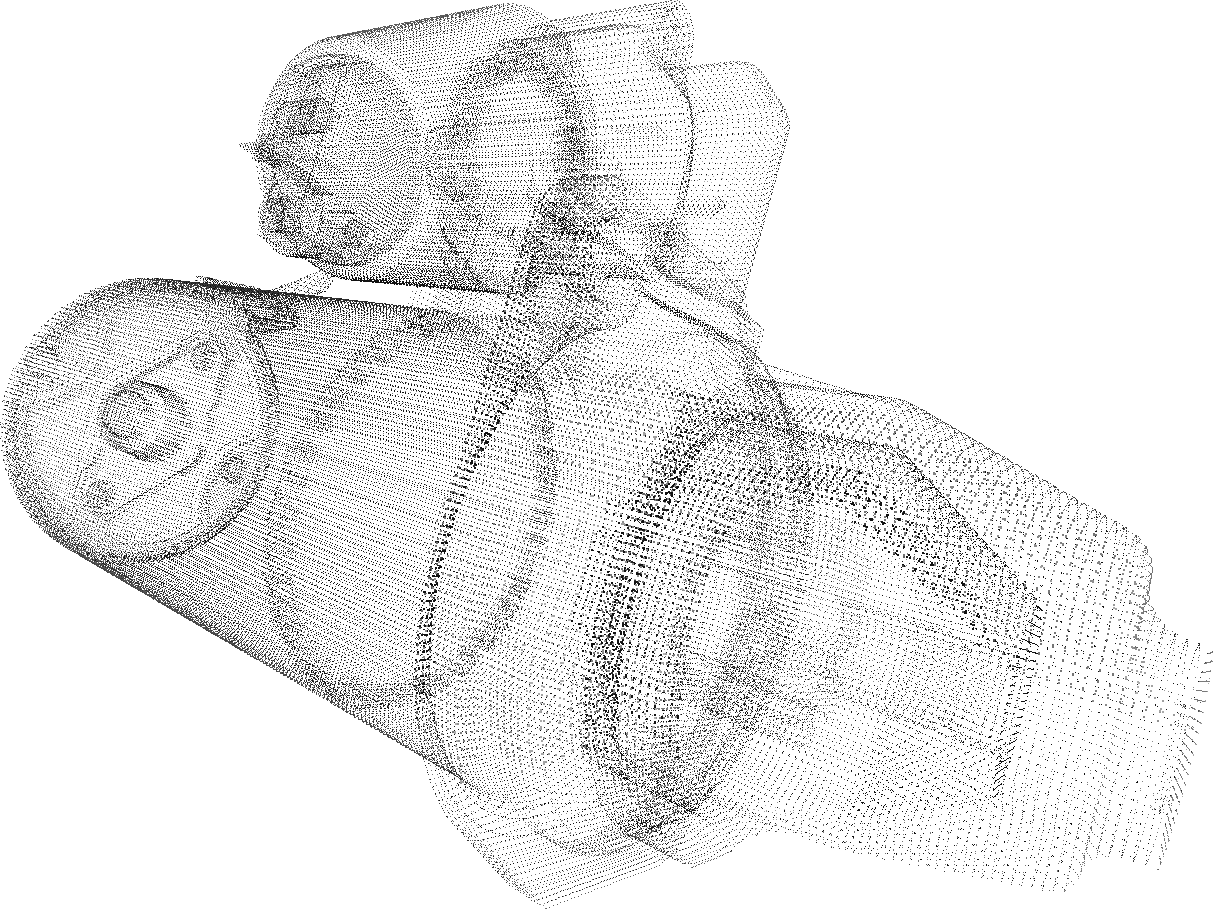
\includegraphics[height=.1\textheight]{sensor-data-processing/cad-model-pointcloud}
	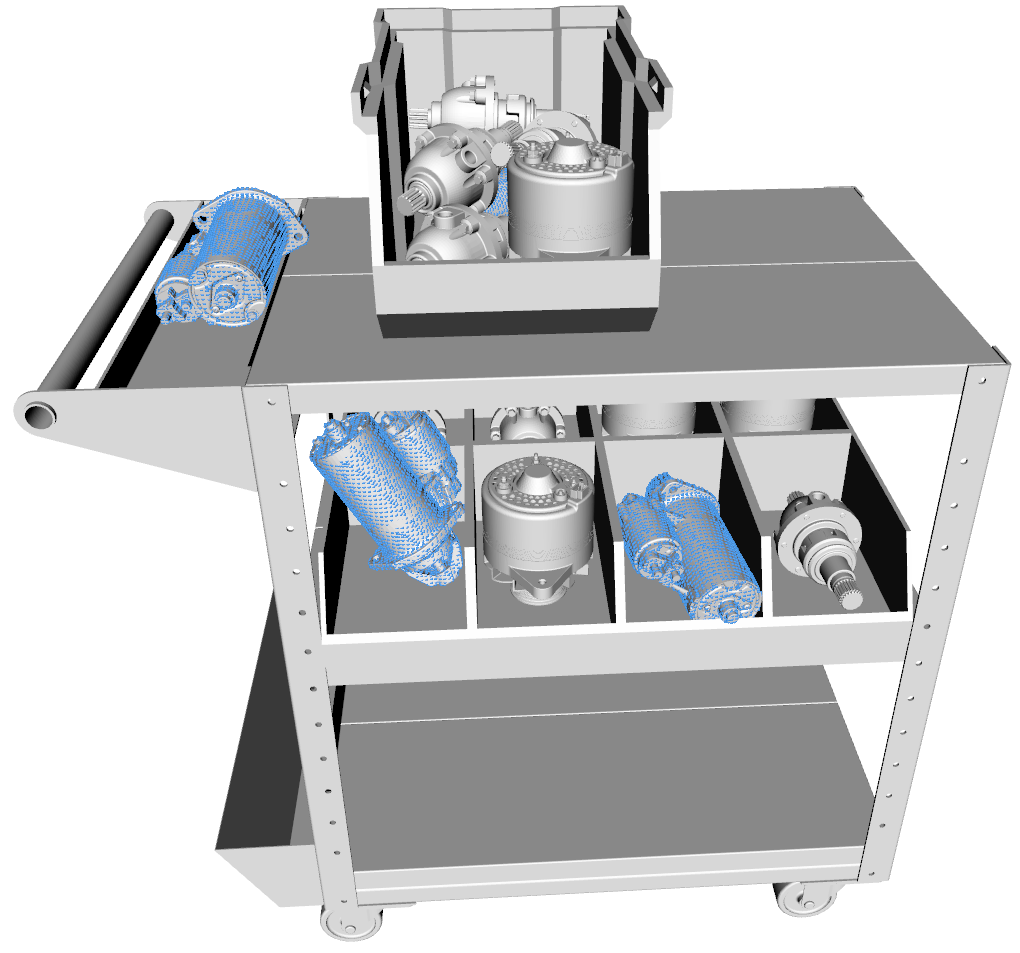
\includegraphics[height=.14\textheight]{sensor-data-processing/multimodel-pointclouds-with-cad}\hspace{2em}
	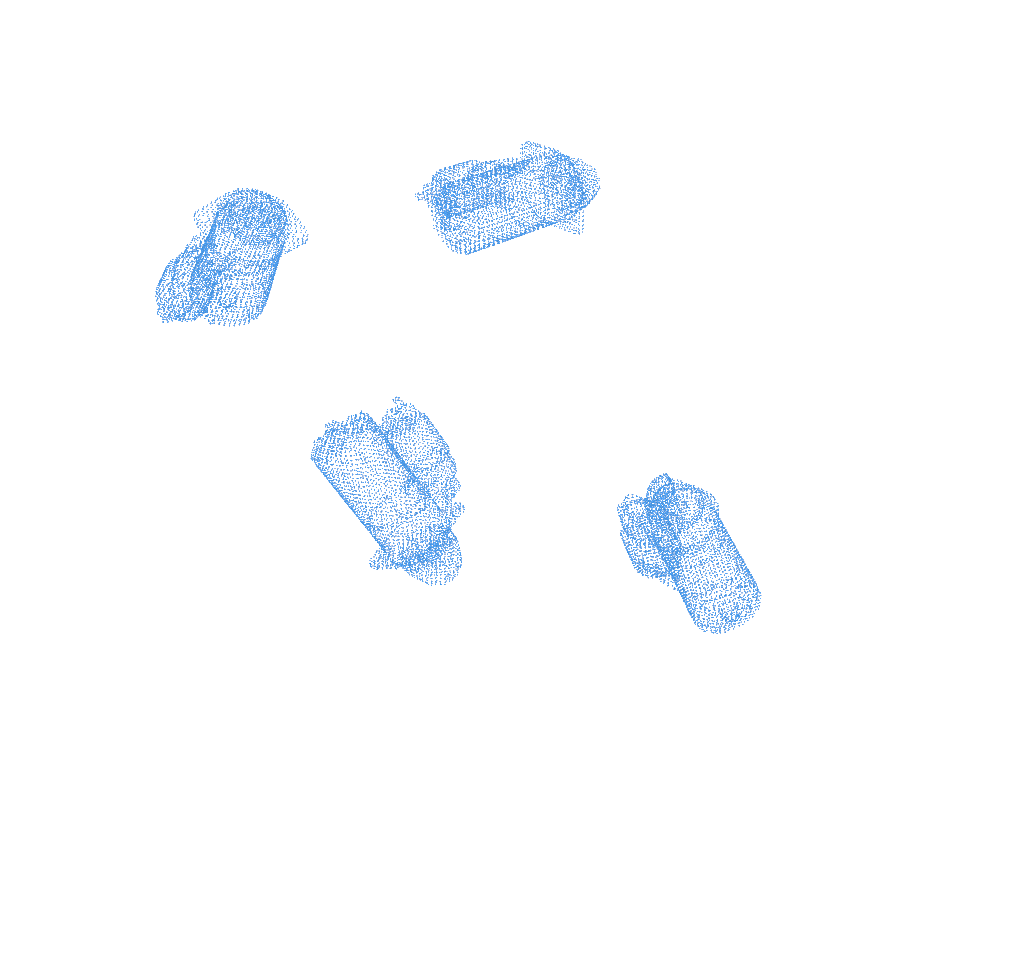
\includegraphics[height=.14\textheight]{sensor-data-processing/multimodel-pointclouds}
	\caption{The first image illustrates the color scene rendering in Gazebo with the target objects in green while the third and fourth images display the reference point cloud that was generated from the CAD points data shown on the second image}
\end{figure}


\subsection{Sensors data analysis}

\begin{itemize}
	\item Given a set of deployed sensors in the simulation world, for each sensor it is computed the voxelized point cloud of the observed target object(s) points:
	\begin{itemize}
		\item Color segmentation is performed to identify the sensor image pixels that belong to the target object(s) (which have a unique pure green material)
		\item For each image pixel associated with a target object, the 3D depth point is computed from the z-buffer depth image using the pinhole camera model
		\item The generated point cloud is transformed from the sensor into the world coordinate system frame
		\begin{itemize}
			\item Allows fast merging of point clouds generated from different sensors
		\end{itemize}
		\item A voxel grid filtering algorithm is applied to perform a regular space partition in which the points centroid are computed for each voxel
		\begin{itemize}
			\item Critical for allowing consistent evaluation of the object(s) observed surface area coverage percentage, even when the sensors have different resolution and are at different distances from the target object(s)
		\end{itemize}
	\end{itemize}
\end{itemize}

\begin{figure}
	\centering
	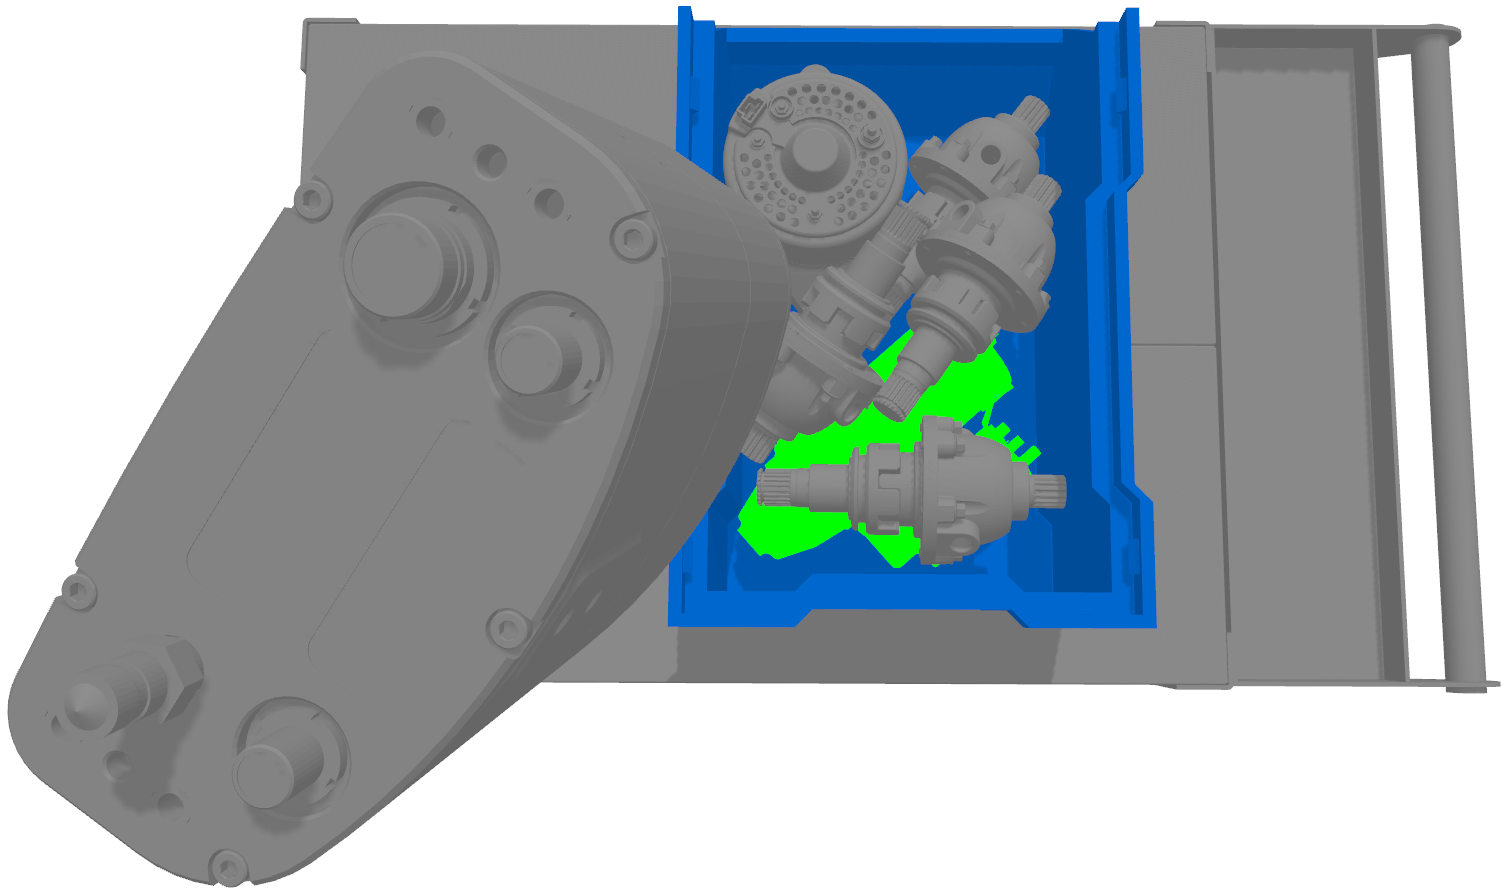
\includegraphics[height=.132\textheight]{sensor-data-processing/sensors-best-view}\\
	\vspace{0.5em}
	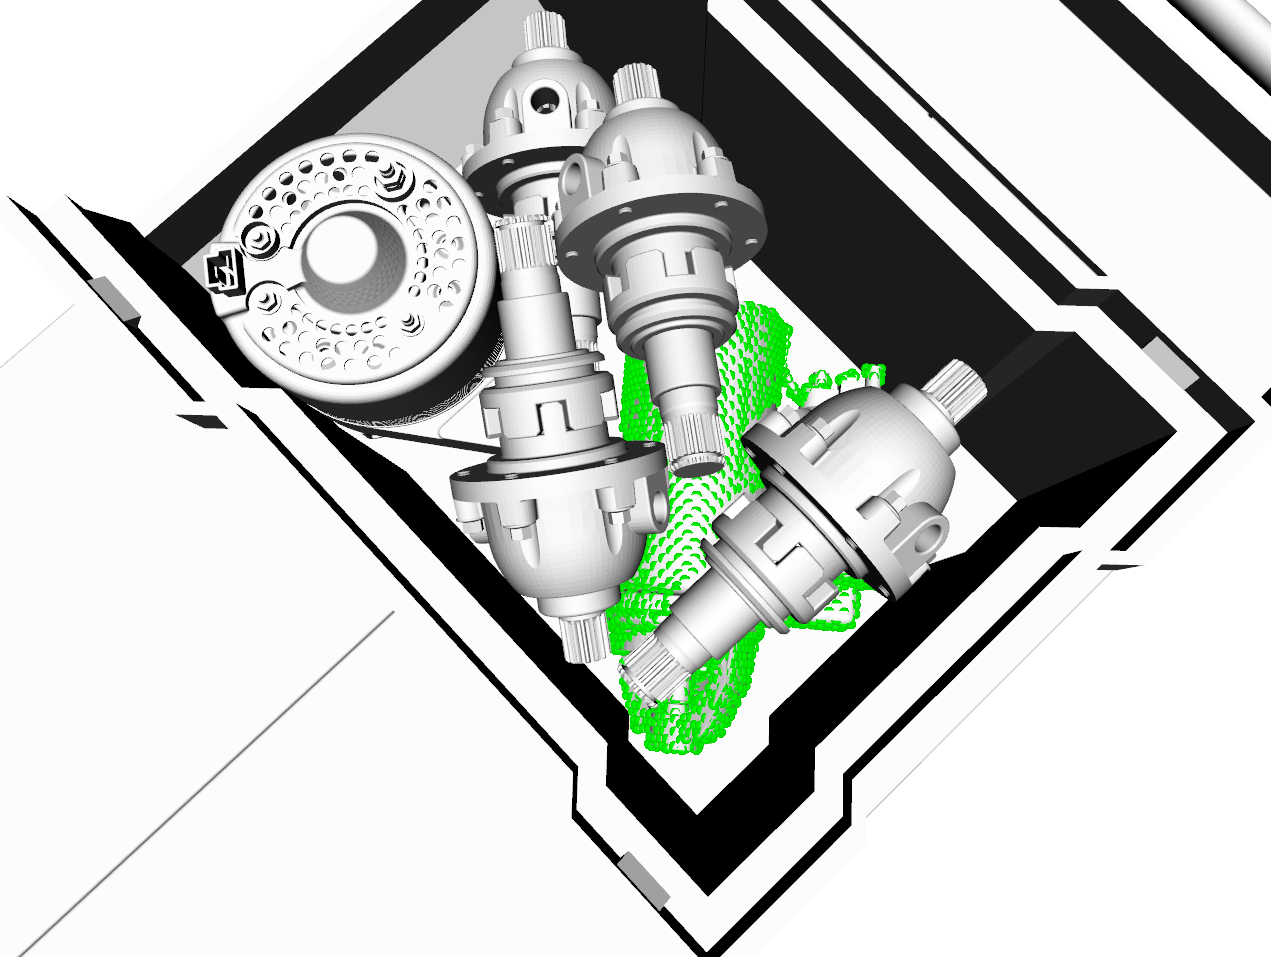
\includegraphics[height=.132\textheight]{sensor-data-processing/rviz-sensor-view}\hspace{2em}
	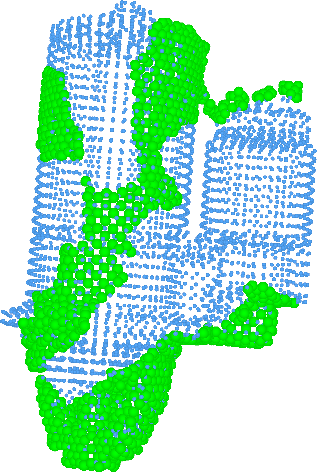
\includegraphics[height=.132\textheight]{sensor-data-processing/rviz-sensor-view-without-cad-with-model}
	\caption{Color image rendered with the Gazebo simulator (top image containing the scene and sensor) along with the generated point cloud for the target object taking into consideration the environment occlusions (bottom images, in which the green spheres are the observed points and the blue spheres are from the point cloud of the associated CAD model)}
\end{figure}


\subsection{Estimation of the best sensor}

After having the processed point cloud for each deployed sensor:
\begin{itemize}
	\item If only one sensor is enough (decision made by the system user):
	\begin{itemize}
		\item The surface coverage percentage for each sensor is computed
		\begin{itemize}
			\item Given that both the reference point cloud and the sensor data were filtered with a voxel grid with the same resolution and in the same coordinate system frame, calculating the surface coverage percentage can be efficiently computed by simply dividing the number of surface voxel points in the sensor data by the number of surface voxel points in the reference point cloud
		\end{itemize}
			\item The sensor that can observe the most surface area percentage of the target object(s) is chosen
	\end{itemize}
\end{itemize}


\subsection{Estimation of the best N sensors disposition}

After having the processed point cloud for each deployed sensor:
\begin{itemize}
	\item If several sensors can be used (decision made by the system user):
	\begin{itemize}
		\item Using a Random Sample Consensus (RANSAC) approach, a set of N sensors is chosen randomly
		\item The sensor data from the selected sensors is merged
		\item The voxel grid filter algorithm is applied to ensure that there is only one point per voxel
		\item The observable surface area percentage for the selected sensors is computed
		\item If the current subset of sensors achieved better observable surface area percentage than the current best, then it becomes the current best views estimation for the sensor disposition
		\item At the end of a given number of iterations or if the observable surface area percentage reaches a given threshold, the search is terminated, returning the best sensor disposition found
	\end{itemize}
\end{itemize}

\section{\uppercase{Experimental evaluation}}\label{sec:results}

\noindent Several tests were conducted in the simulated environments presented earlier for evaluating the ability of the proposed system to find suitable constellations of sensors for maximizing the observable surface area of a given set of target objects.

In the active perception environment introduced in \cref{fig:active-perception-environment}, it was performed two tests with the sensor deployment shown in \cref{fig:sensors-deployment-active-perception-environment}. In the first test it was estimated the best sensor position for observing a single target object (green starter motor) being occluded by a human hand starting to grasp it. By visually inspecting the scene in \cref{fig:active-perception-1-sensor}, it can be seen that the system chose a very reasonable sensor position, achieving a surface coverage of 27.73\%, despite the heavy occlusions present. Moreover, when expanding the number of sensors to 3 (in the second test), the system managed to select a sensor constellation with a good spatial distribution (shown in \cref{fig:active-perception-3-sensors}) that managed to improve the sensor coverage to 61.91\%.

Moving to the single bin picking environments, presented in \cref{fig:bin-picking-environment,fig:bin-picking-with-occlusions-environment}, it was made four more tests using the deployed sensors seen in \cref{fig:sensors-deployment-bin-picking-environments}. In the first test it was estimated the best position for a single sensor to observe the target object that was inside the stacking box, which had large occlusions on its surroundings, but could be clearly observed from above. As can be seen in \cref{fig:bin-picking-1-sensor}, the system choose a suitable observation sensor that managed to achieve a surface coverage of 45.10\%. When increasing the number of sensors to 5 (in the second test), the system relied on more sensor data and improved the surface coverage to 64.63\%. To make the active perception for this bin picking use case more challenging, it was added three occluding differential gearboxes on top of the target object (scene shown on \cref{fig:bin-picking-with-occlusions-environment}) in order to create large occlusions that significantly reduced the number of useful sensors in the deployed populations (presented in \cref{fig:sensors-deployment-bin-picking-environments}). Analyzing the best sensor position estimated by the system (shown in \cref{fig:sensor-data-processing,fig:bin-picking-with-occlusions-1-sensor}) it can be seen that the pose chosen was very reasonable, achieving a surface coverage of 19.27\%. When increasing the number of sensors to 3, the system deployed a constellation with good spatial distribution and managed to improved the surface coverage percentage of the target object to 31.19\% (as can be seen in \cref{fig:bin-picking-with-occlusions-3-sensors}).

Increasing the level of complexity even further, in the final test it was added three more target objects to the simulation environment (as presented in \cref{fig:multiple-bin-picking-with-occlusions-environment}) and the number of populations with different sensor types was increased to 7 (shown in \cref{fig:sensors-deployment-multiple-bin-picking-environment}). Analyzing \cref{fig:multiple-bin-picking-with-occlusions-10-sensors} in which the system estimated a constellation of 10 sensors to observe the 4 target objects, it can be seen that the system chose 4 sensors on the front wall (which had a better observation area for the target objects in the trolley shelves), 3 on the ceiling (for retrieving sensor data for the target objects on top of the trolley) and then for observing the remaining surface areas of the target objects, it chose one sensor on the left wall, another on the right wall and finally another one on the back wall, reaching 10 sensors in total and achieving a surface coverage of the target objects of 43.93\%.

These 7 constellations of sensors computed using \cref{alg:best-n-views} (which relied on a \gls{ransac} approach), show that the proposed system can estimate a suitable sensor configuration for maximizing the observable surface area of several target objects even on complex environments with significant occlusions. Moreover, the system managed to compute useful solutions in bounded and reasonable time (from less than a second to a few minutes depending on the number and characteristics of the deployed sensors) for a problem that is combinatorial explosive in terms of processing time complexity.

\begin{figure}
	\centering
	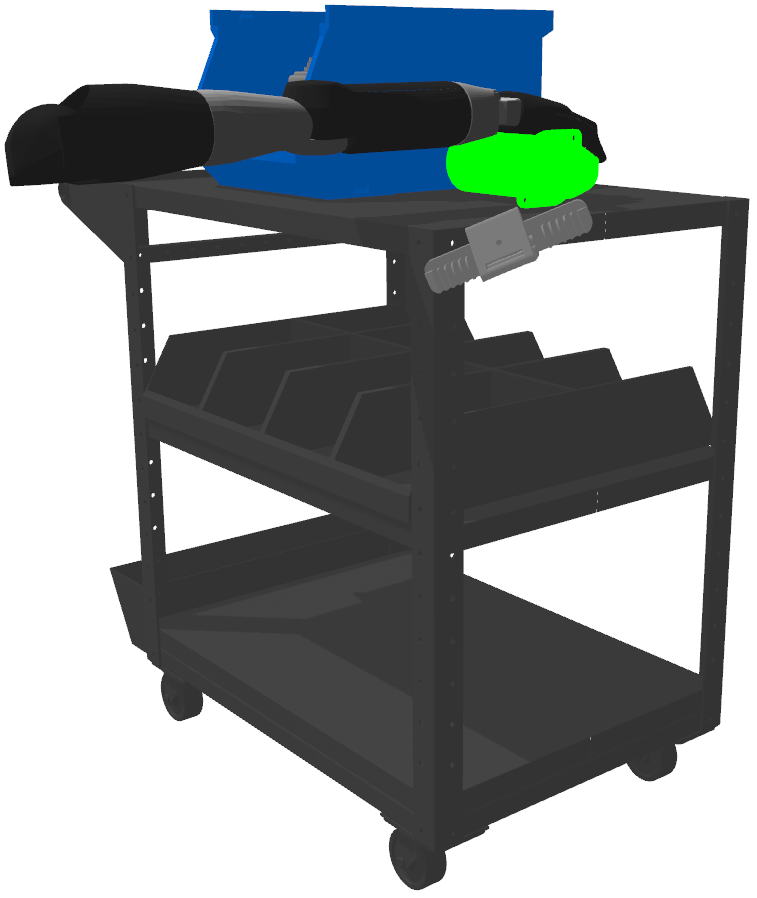
\includegraphics[height=.2\textwidth]{best-views-estimation/active-perception/1-sensor/gazebo-corner}\hspace{4em}
	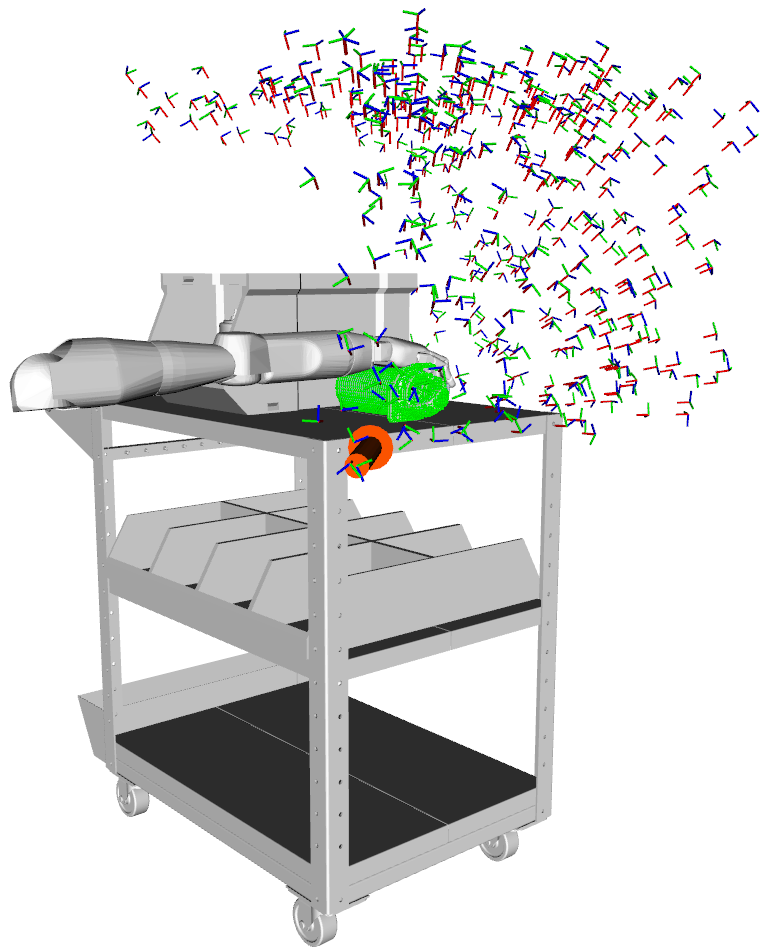
\includegraphics[height=.2\textwidth]{best-views-estimation/active-perception/1-sensor/rviz-front-corner}\\
	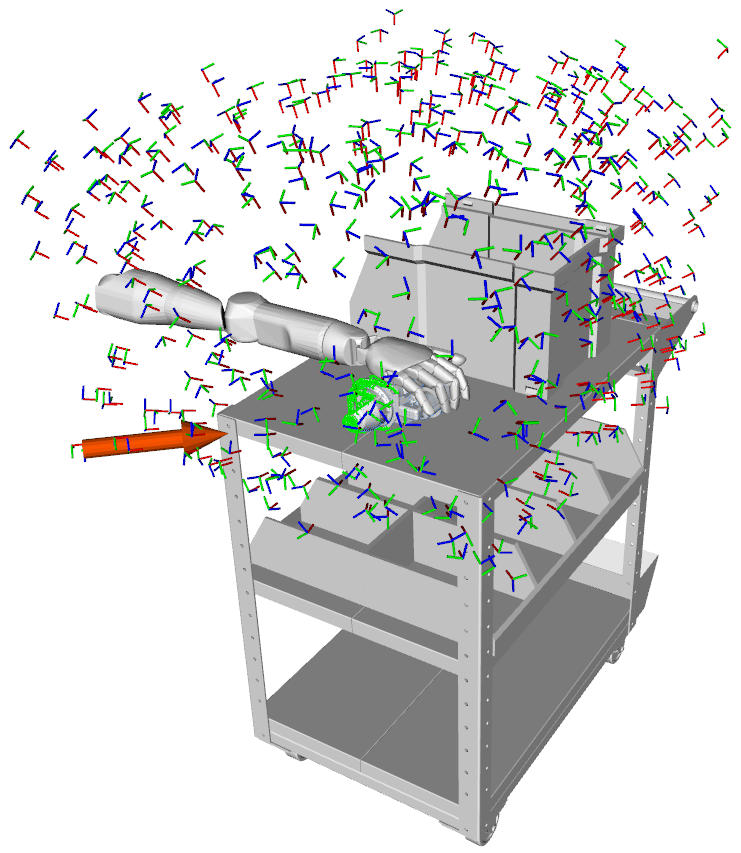
\includegraphics[height=.2\textwidth]{best-views-estimation/active-perception/1-sensor/rviz-back-corner}\hspace{2em}
	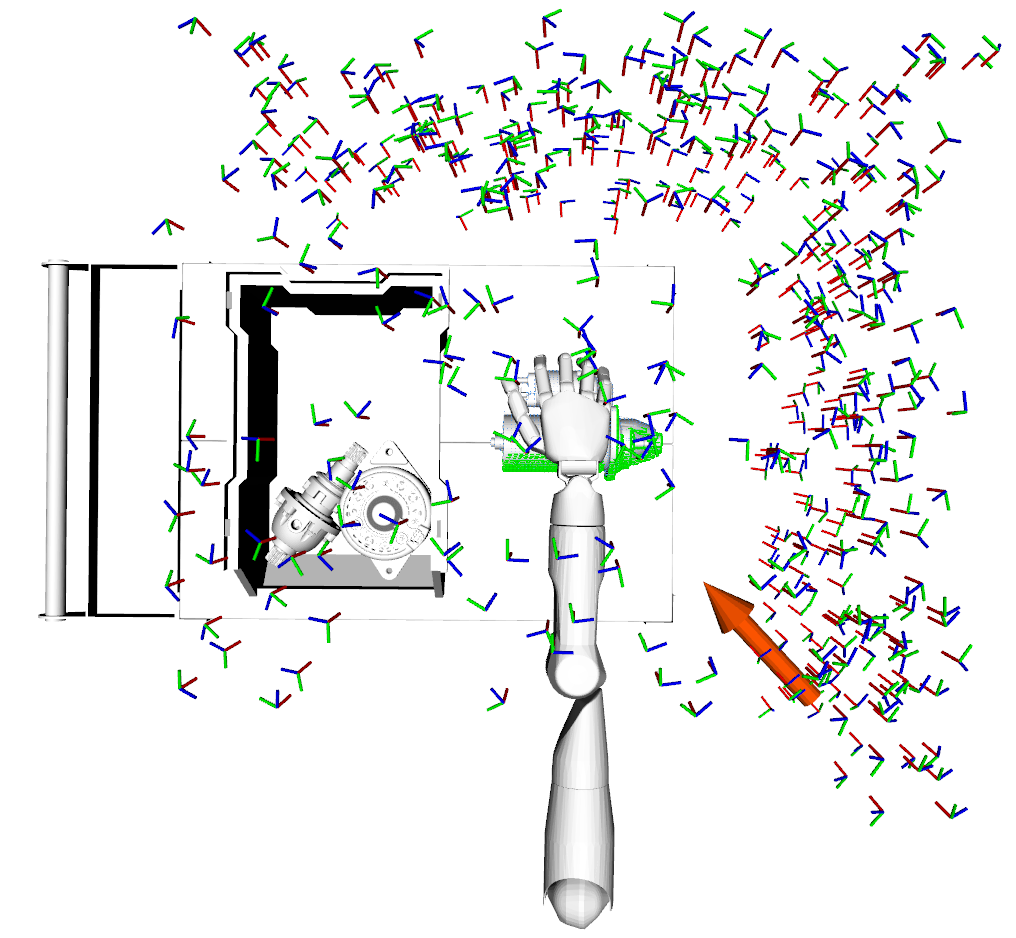
\includegraphics[height=.2\textwidth]{best-views-estimation/active-perception/1-sensor/rviz-top}
	\caption{Estimation of the best sensor position for the active perception environment with a 27.73\% of surface area coverage (top left showing the Gazebo color rendering and remaining images displaying the best sensor as a large red arrow, the deployed sensors as small coordinate frames and the observed sensor data as green spheres).}
	\label{fig:active-perception-1-sensor}
\end{figure}

\begin{figure}
	\centering
	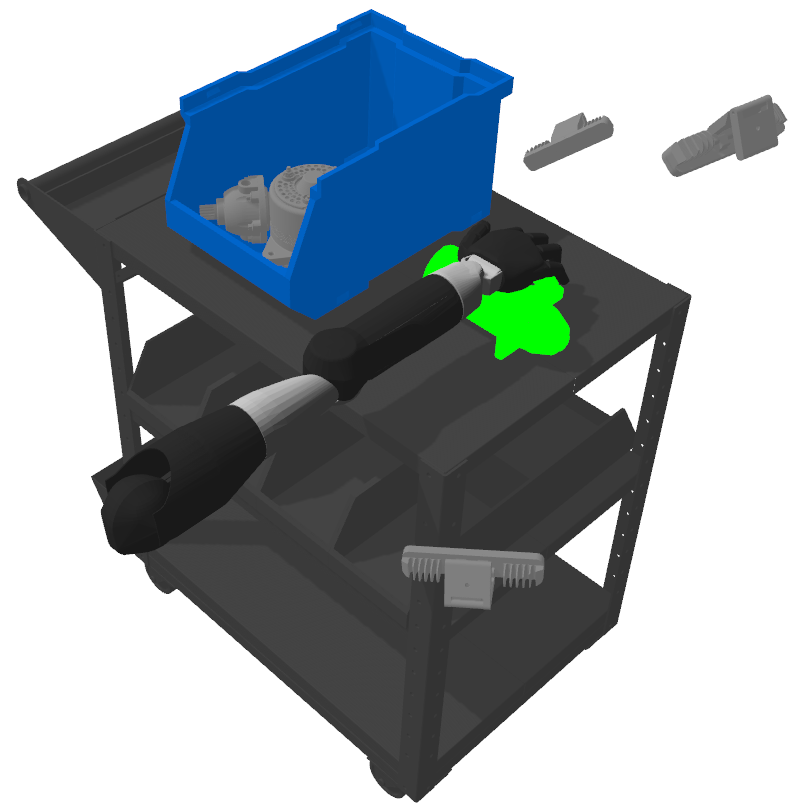
\includegraphics[height=.2\textwidth]{best-views-estimation/active-perception/3-sensors/gazebo-front-right-corner}\hspace{4em}
	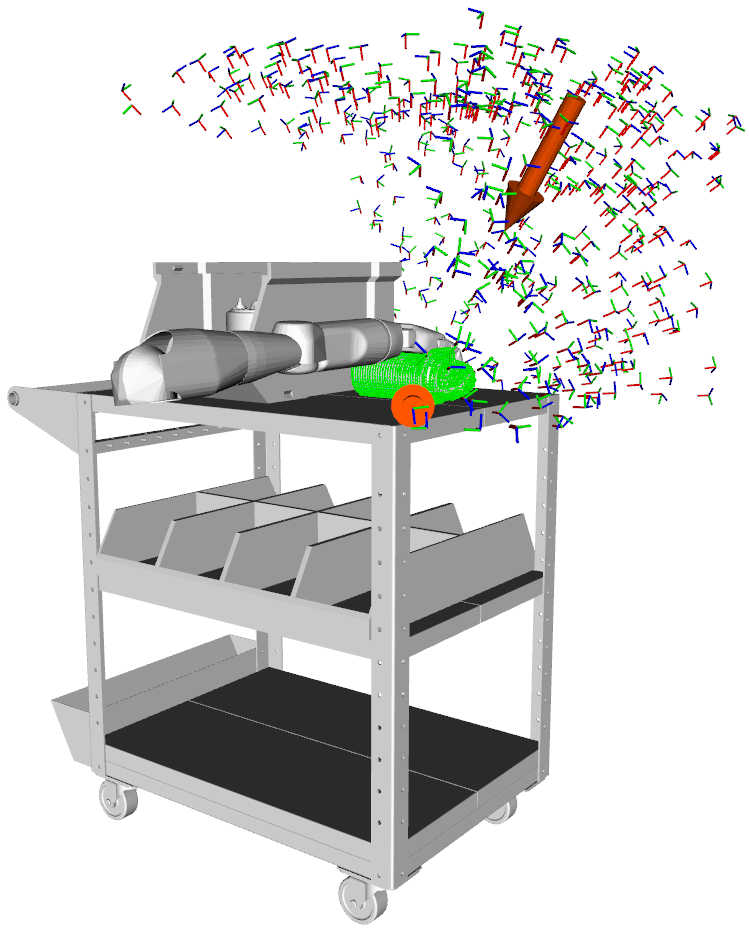
\includegraphics[height=.2\textwidth]{best-views-estimation/active-perception/3-sensors/rviz-front-right}\\
	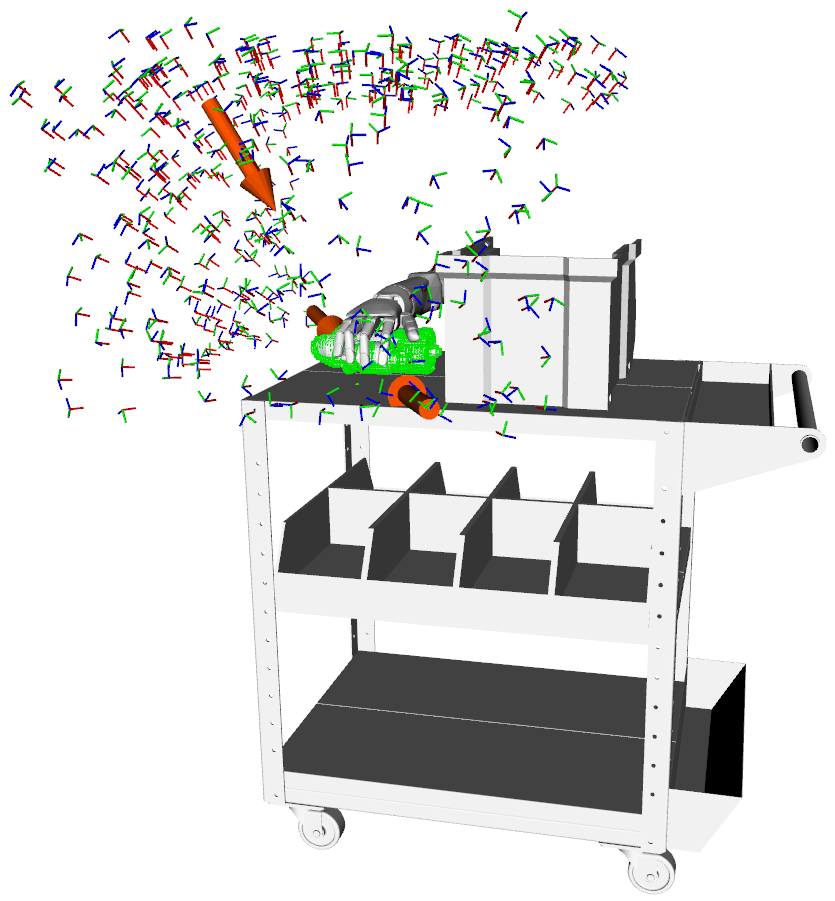
\includegraphics[height=.2\textwidth]{best-views-estimation/active-perception/3-sensors/rviz-back-left}\hspace{2em}
	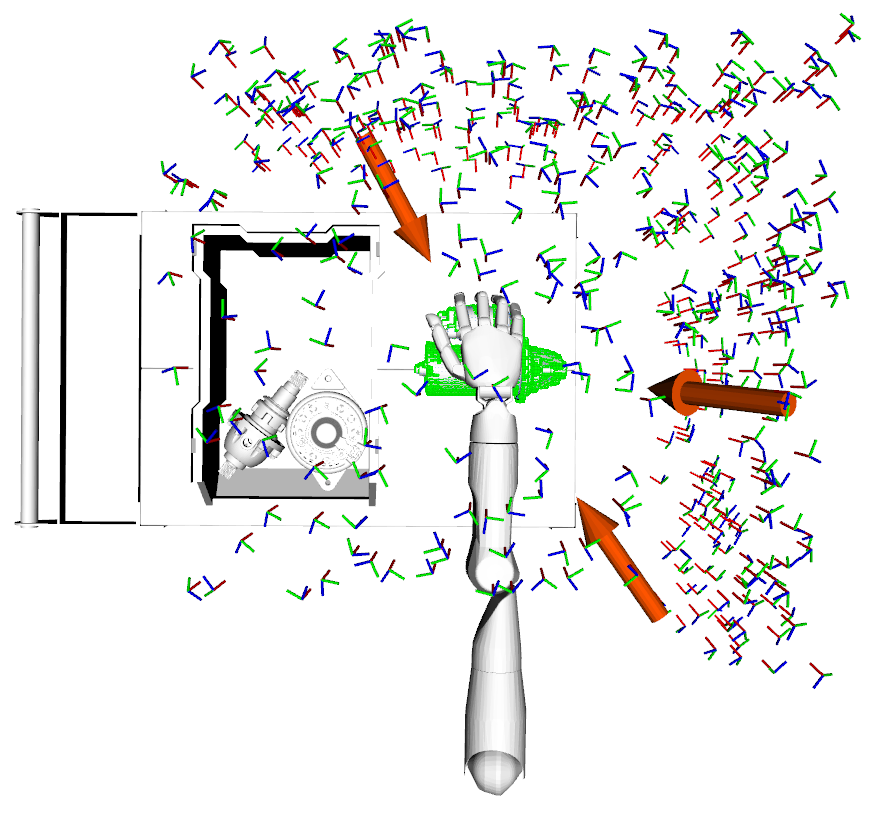
\includegraphics[height=.2\textwidth]{best-views-estimation/active-perception/3-sensors/rviz-top}
	\caption{Estimation of the 3 best sensors disposition for the active perception environment with a 61.91\% of surface area coverage.}
	\label{fig:active-perception-3-sensors}
\end{figure}

\begin{figure}
	\centering
	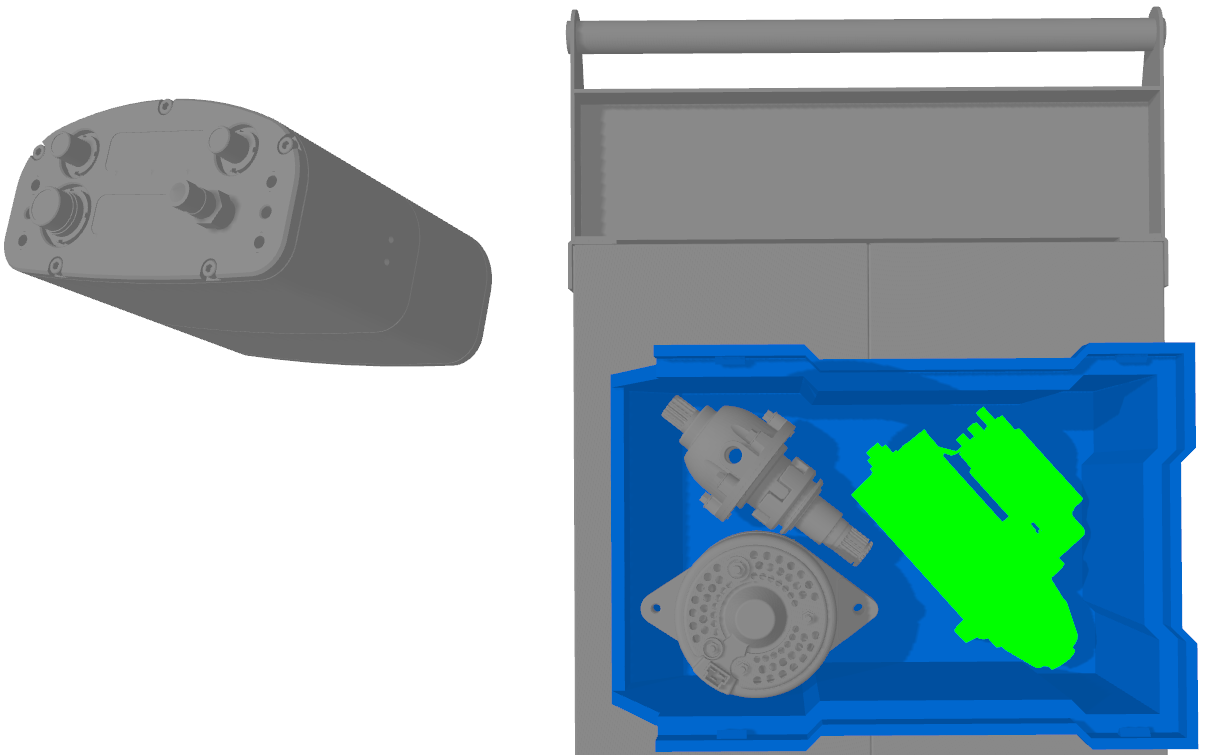
\includegraphics[height=.14\textwidth]{best-views-estimation/bin-picking/1-sensor/gazebo-top}\hspace{2em}
	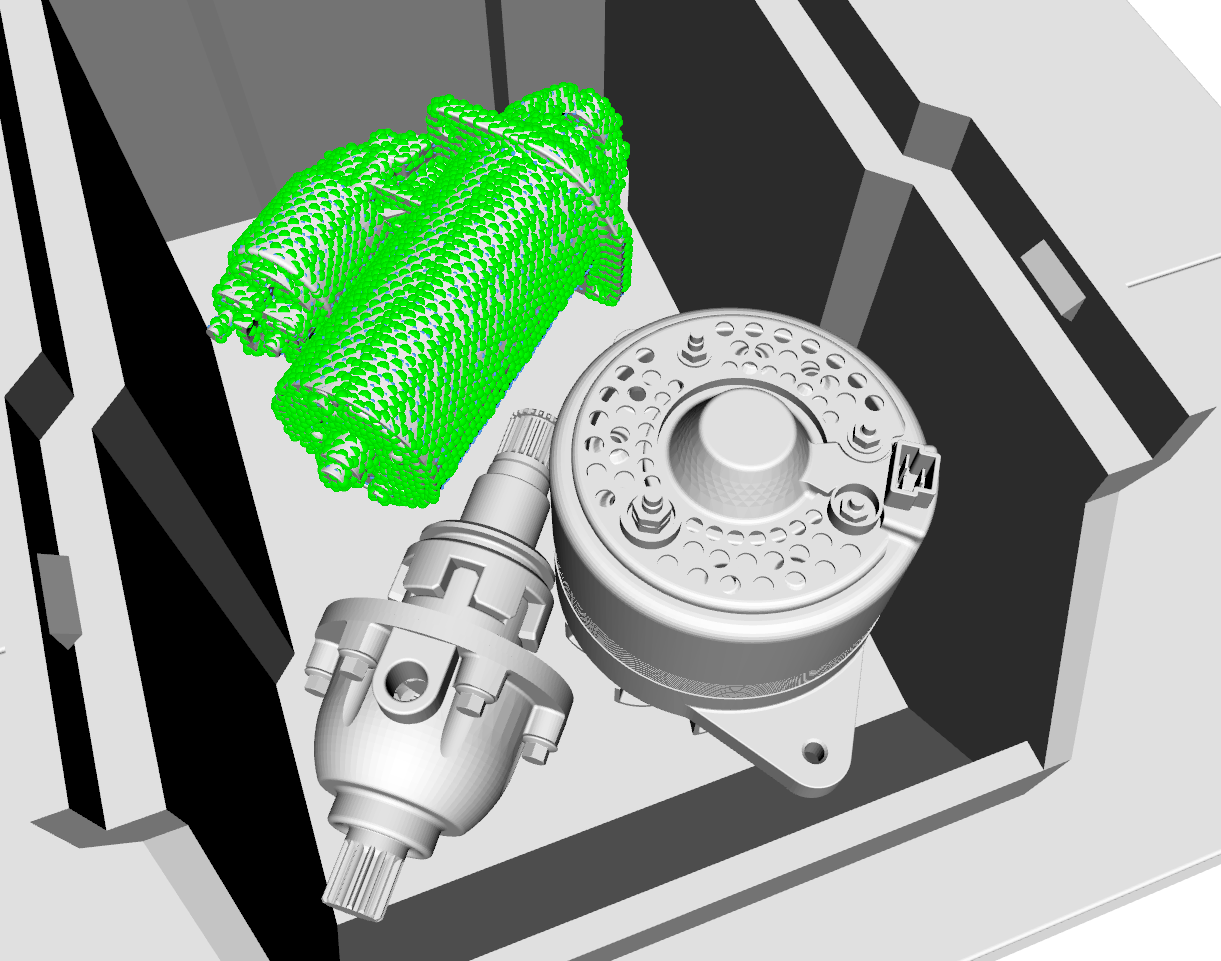
\includegraphics[height=.14\textwidth]{best-views-estimation/bin-picking/1-sensor/rviz-front}\\
	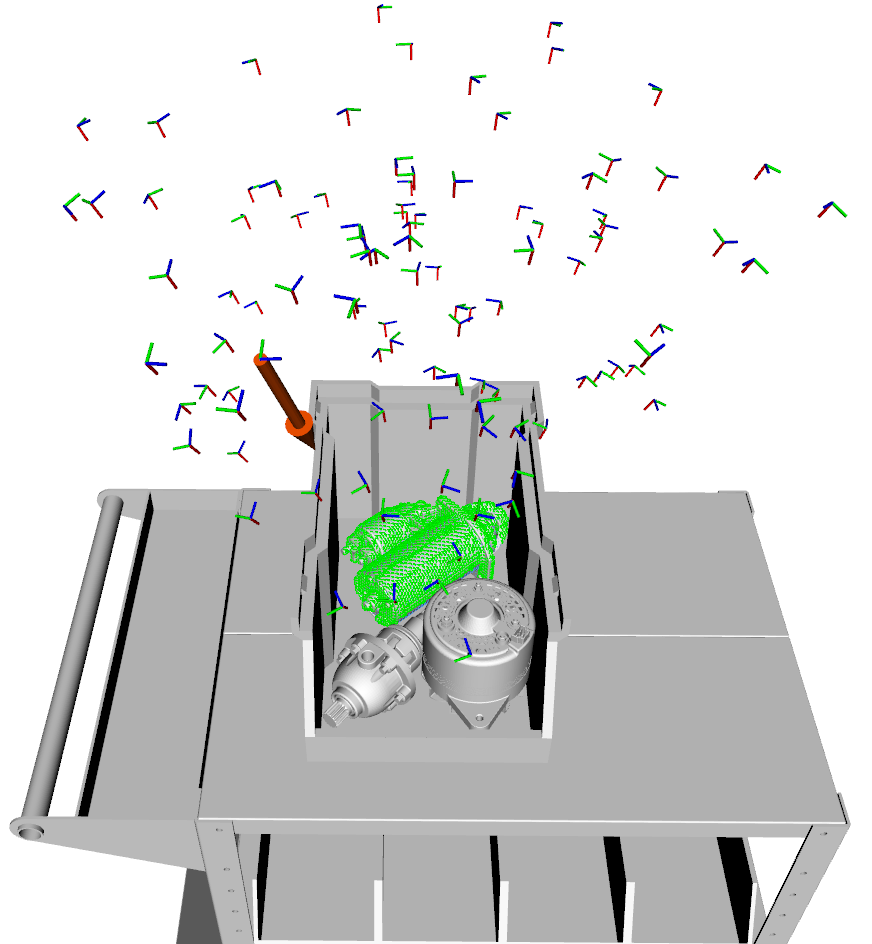
\includegraphics[height=.2\textwidth]{best-views-estimation/bin-picking/1-sensor/rviz-top-front}\hspace{2em}
	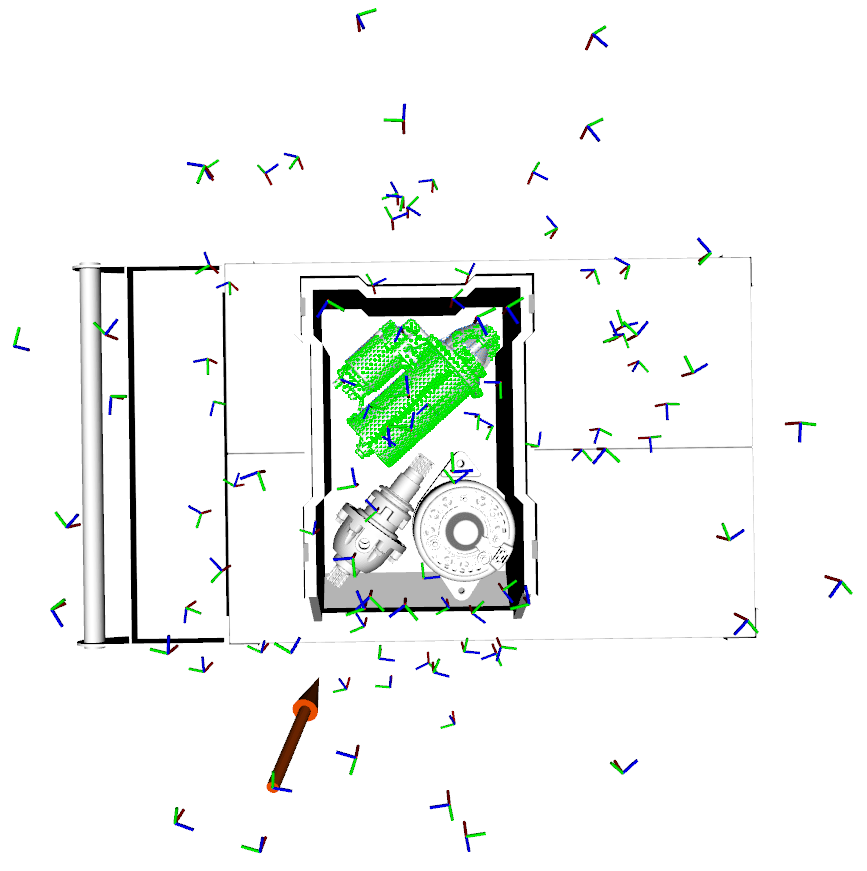
\includegraphics[height=.2\textwidth]{best-views-estimation/bin-picking/1-sensor/rviz-top}
	\caption{Estimation of the best sensor position for the bin picking environment with a 45.10\% of surface area coverage.}
	\label{fig:bin-picking-1-sensor}
\end{figure}

\begin{figure}
	\centering
	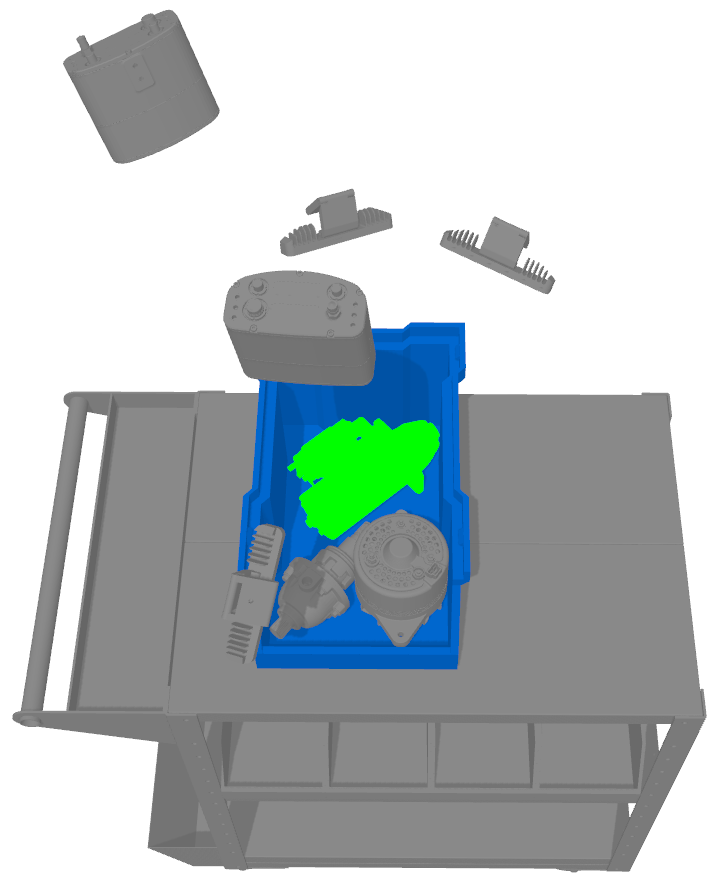
\includegraphics[height=.19\textwidth]{best-views-estimation/bin-picking/5-sensors/gazebo-front}\hspace{2em}
	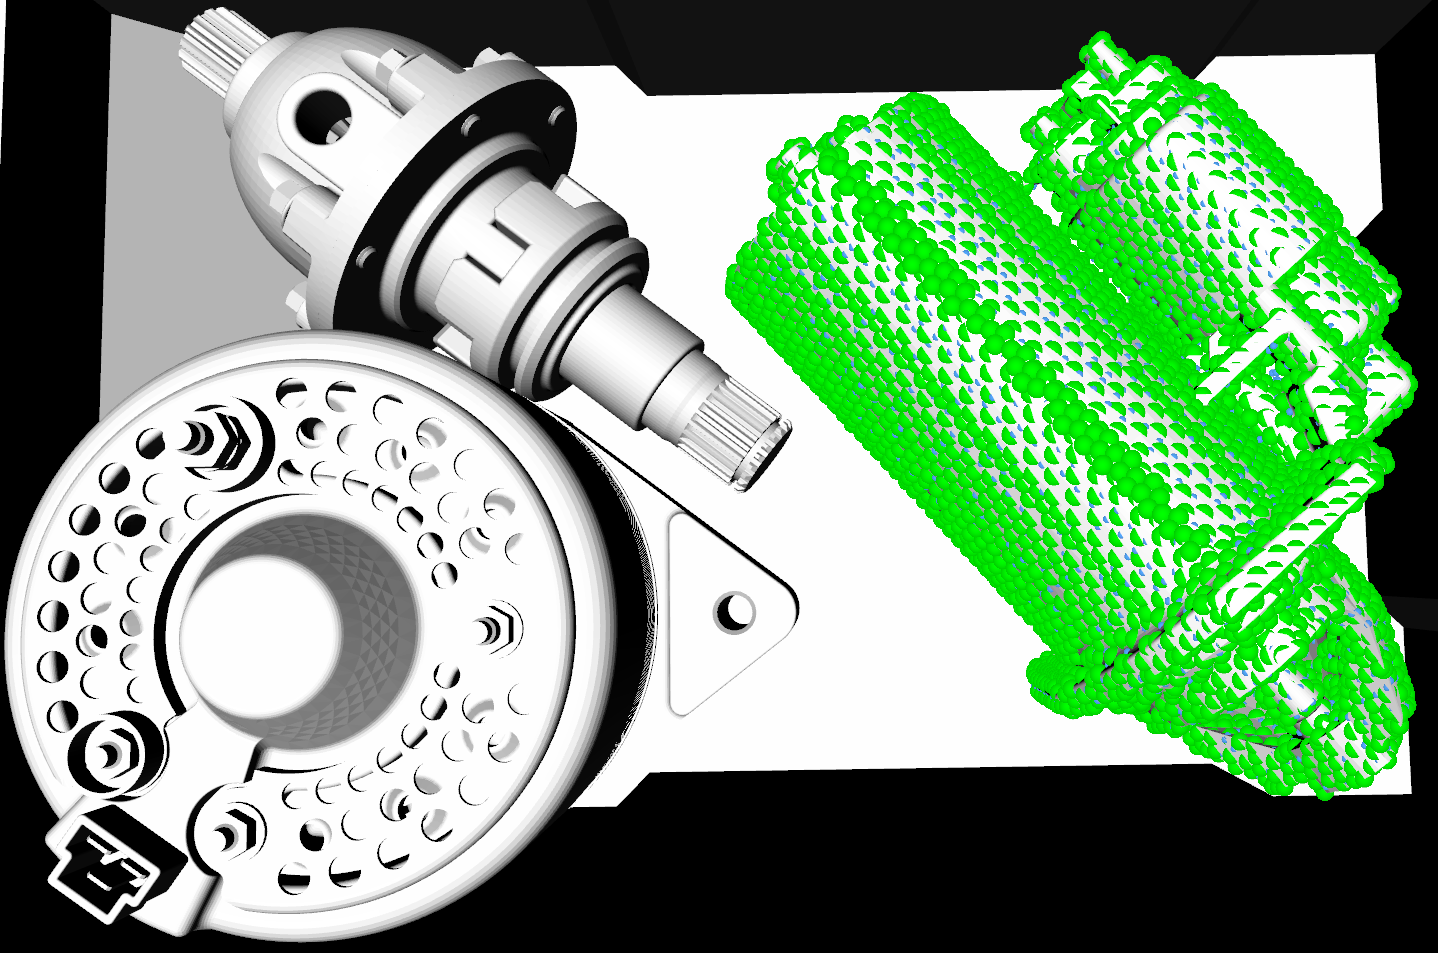
\includegraphics[height=.14\textwidth]{best-views-estimation/bin-picking/5-sensors/rviz-top}\\
	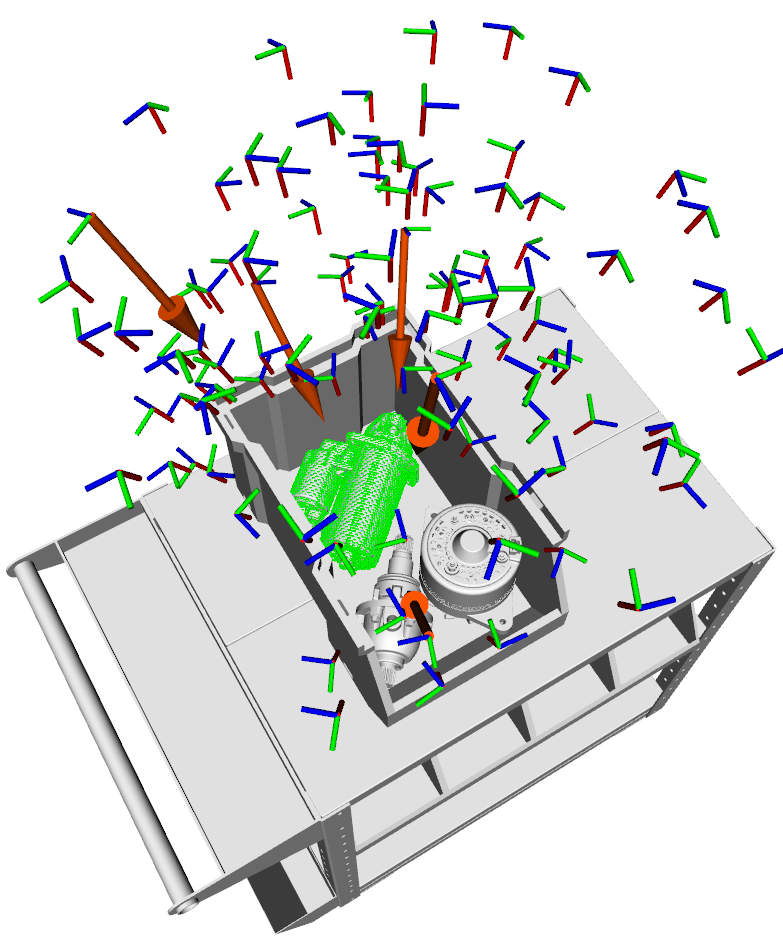
\includegraphics[height=.2\textwidth]{best-views-estimation/bin-picking/5-sensors/rviz-corner}\hspace{2em}
	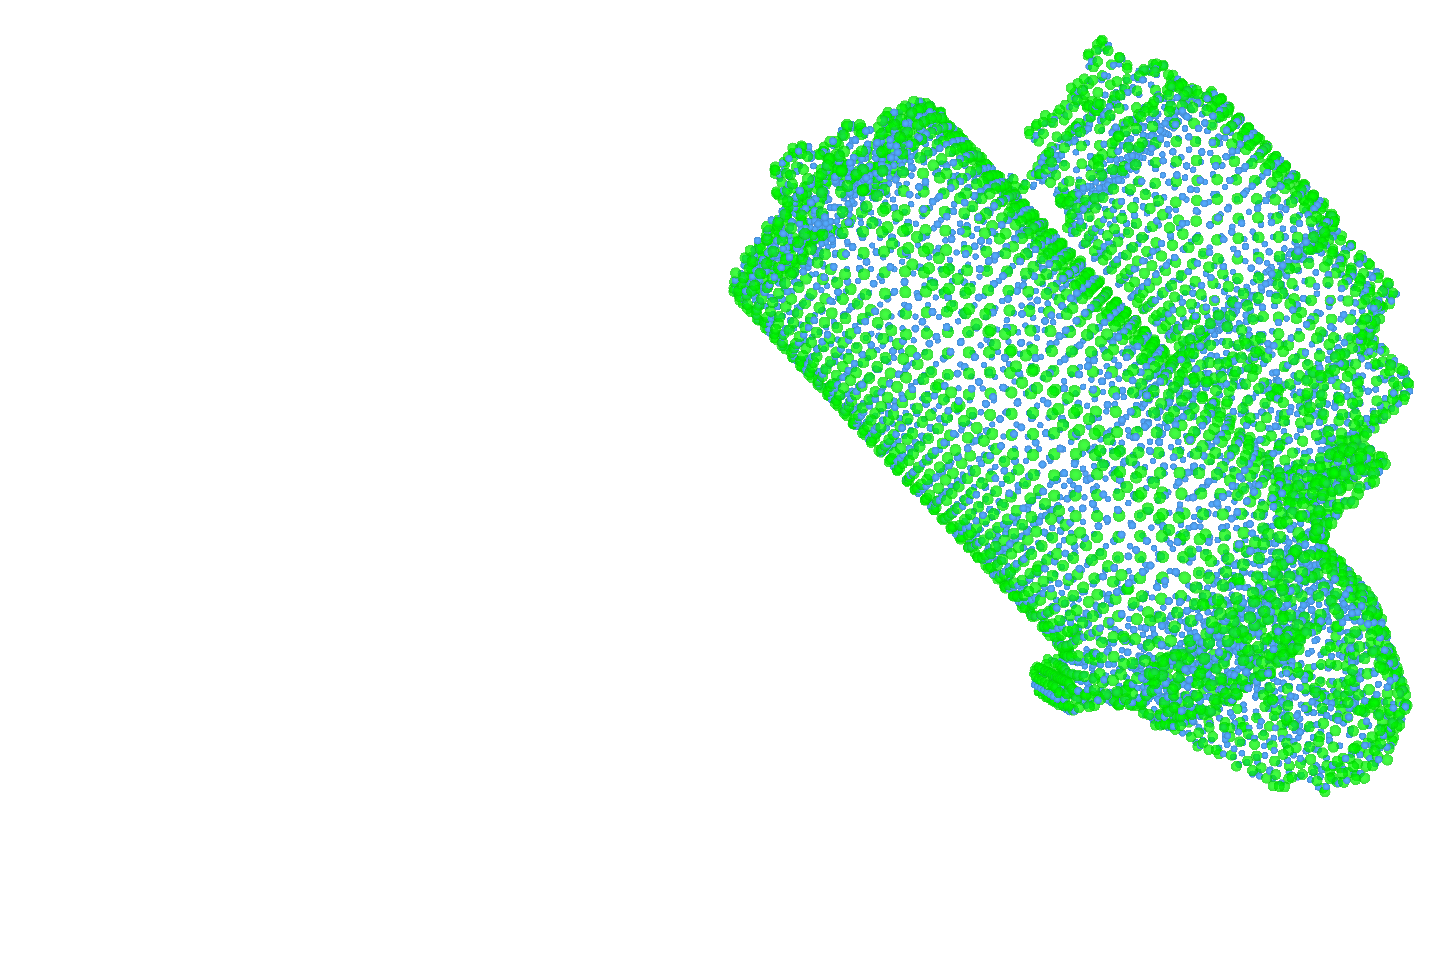
\includegraphics[height=.14\textwidth]{best-views-estimation/bin-picking/5-sensors/rviz-sensor-data}
	\caption{Estimation of the 5 best sensors disposition for the bin picking environment with a 64.63\% of surface area coverage.}
	\label{fig:bin-picking-5-sensors}
\end{figure}

\begin{figure}
	\centering
	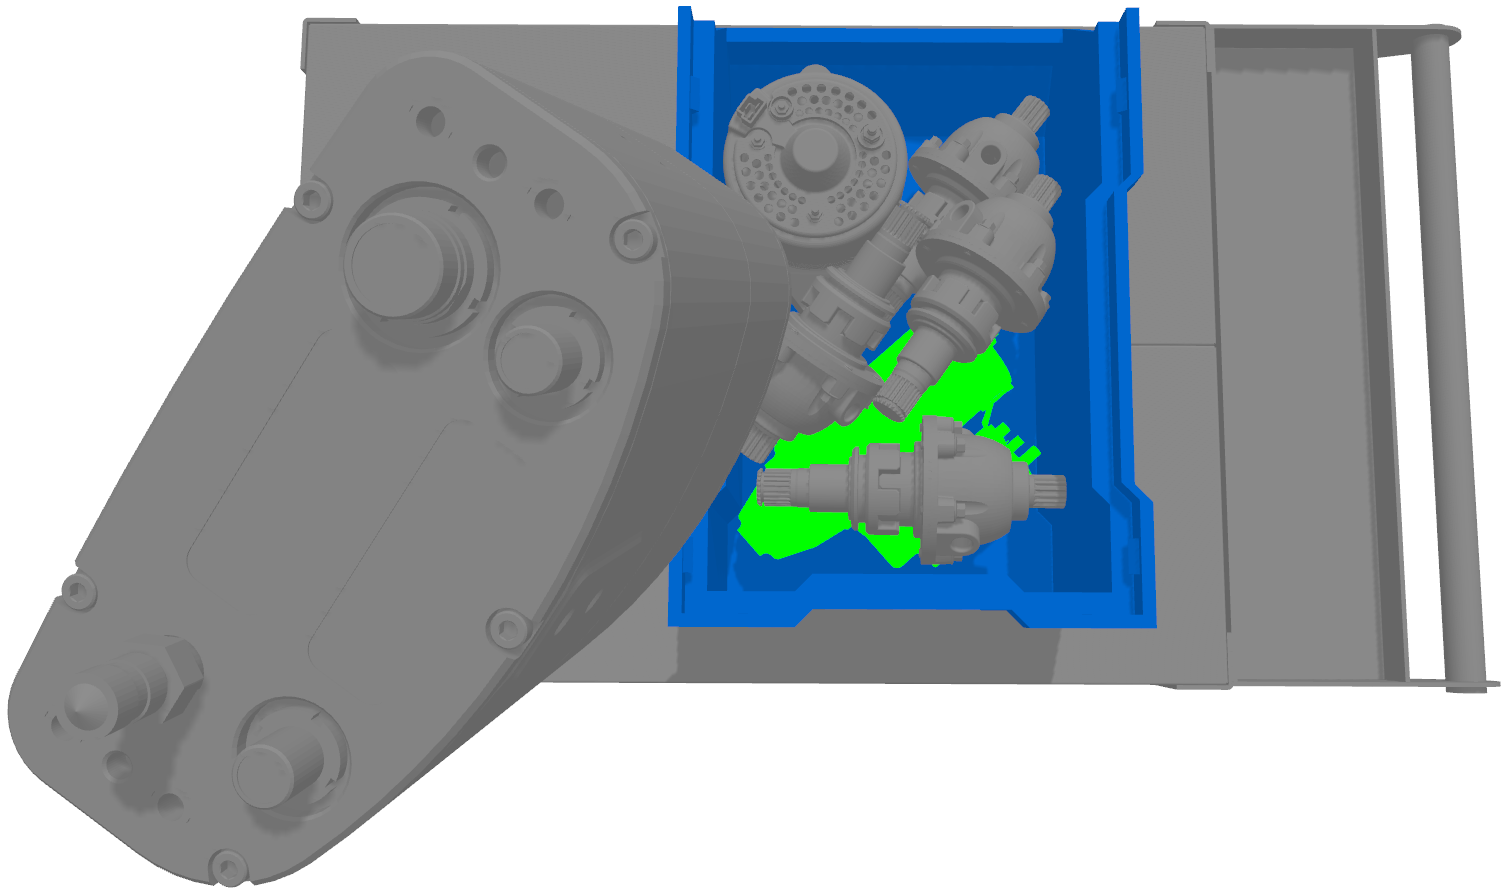
\includegraphics[height=.13\textwidth]{best-views-estimation/bin-picking-with-occlusions/1-sensor/gazebo-top}\hspace{2em}
	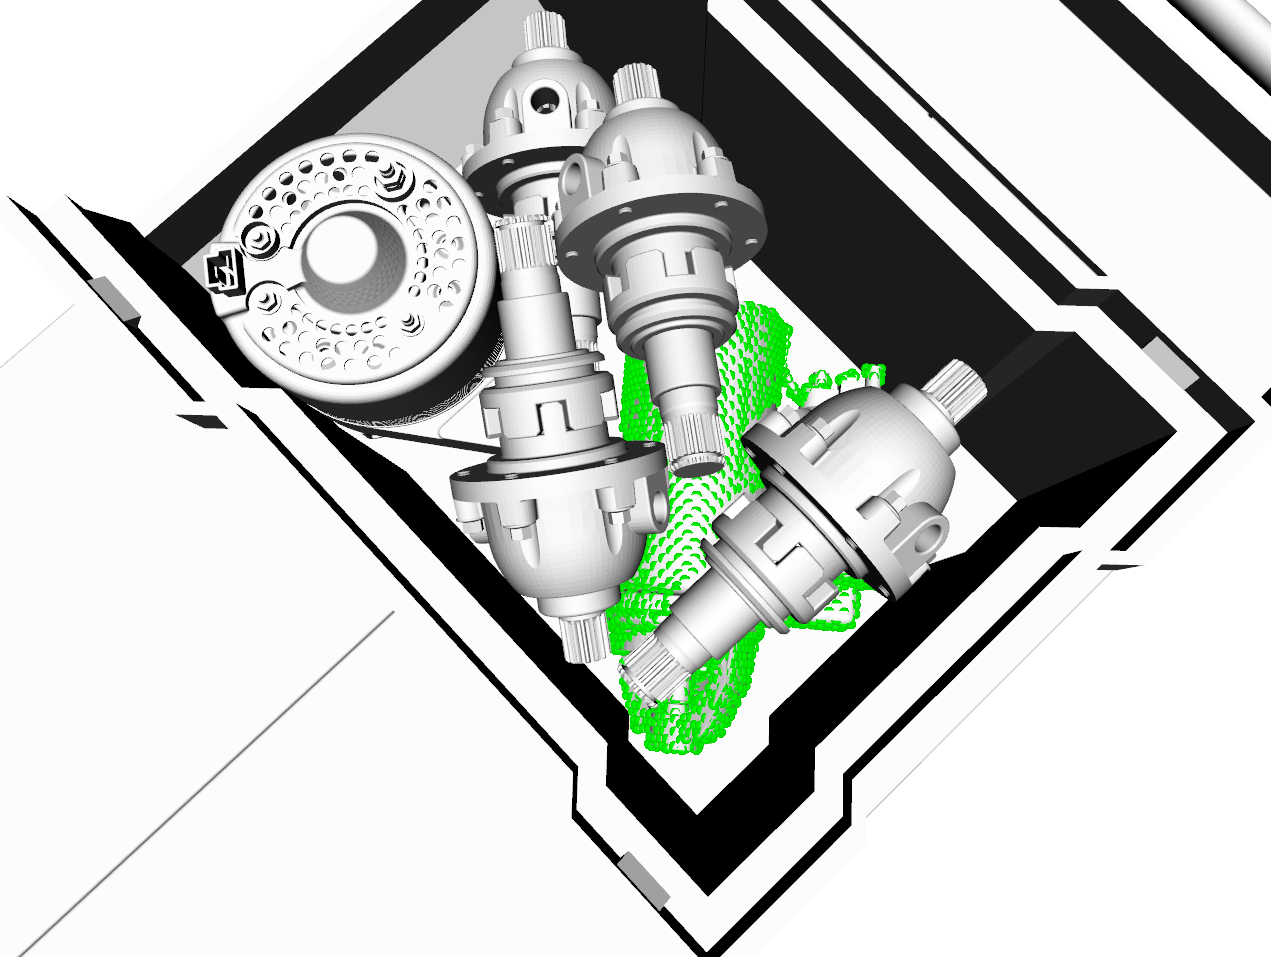
\includegraphics[height=.13\textwidth]{best-views-estimation/bin-picking-with-occlusions/1-sensor/rviz-corner}\\
	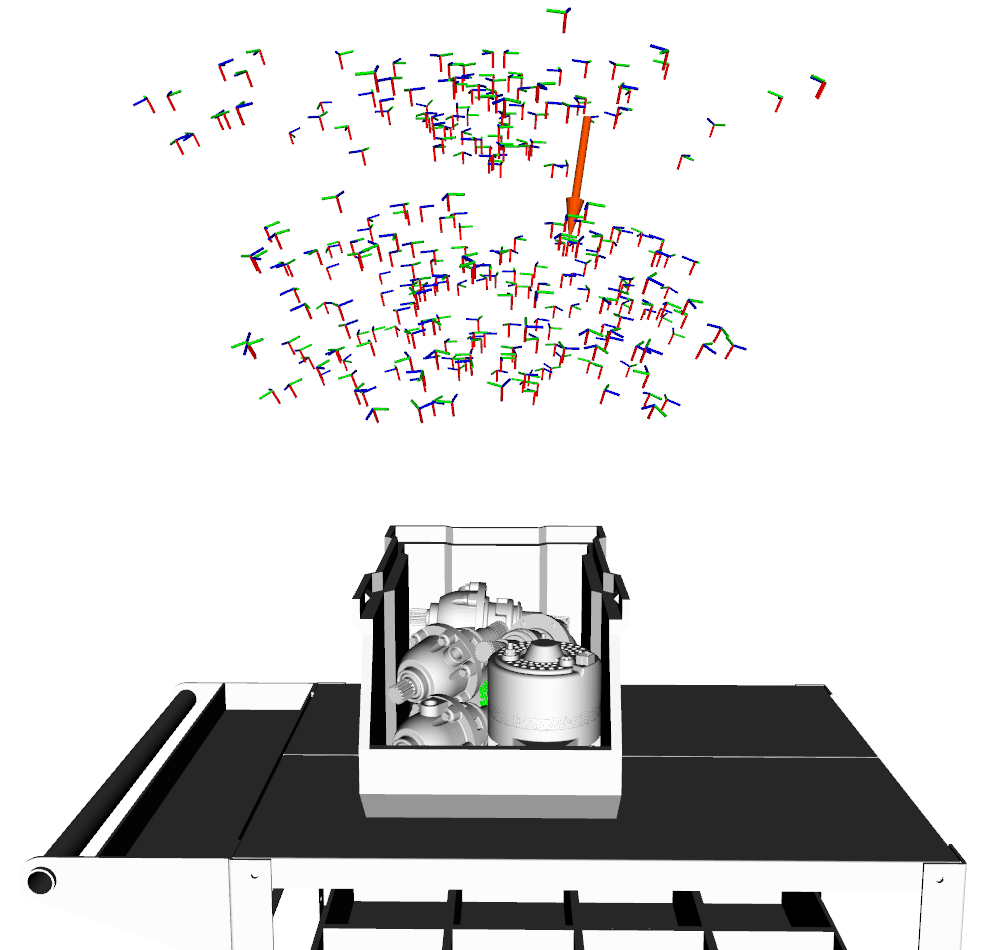
\includegraphics[height=.2\textwidth]{best-views-estimation/bin-picking-with-occlusions/1-sensor/rviz-front}\hspace{2em}
	\includegraphics[height=.2\textwidth]{best-views-estimation/bin-picking-with-occlusions/1-sensor/rviz-top}
	\caption{Estimation of the best sensor position for the bin picking with occlusions environment with a 19.27\% of surface area coverage.}
	\label{fig:bin-picking-with-occlusions-1-sensor}
\end{figure}

\begin{figure}
	\centering
	\includegraphics[height=.18\textwidth]{best-views-estimation/bin-picking-with-occlusions/3-sensors/gazebo-top}\hspace{2em}
	\includegraphics[height=.2\textwidth]{best-views-estimation/bin-picking-with-occlusions/3-sensors/rviz-front}\\
	\includegraphics[height=.21\textwidth]{best-views-estimation/bin-picking-with-occlusions/3-sensors/rviz-top-back}\hspace{2em}
	\includegraphics[height=.21\textwidth]{best-views-estimation/bin-picking-with-occlusions/3-sensors/rviz-top}
	\caption{Estimation of the 3 best sensors disposition for the bin picking with occlusions environment with a 31.19\% of surface area coverage.}
	\label{fig:bin-picking-with-occlusions-3-sensors}
\end{figure}

\begin{figure}
	\centering
	\includegraphics[width=.49\textwidth]{best-views-estimation/multiple-bin-picking-with-occlusions/10-sensors/gazebo-front}\vspace{2em}
	\includegraphics[width=.25\textwidth]{best-views-estimation/multiple-bin-picking-with-occlusions/10-sensors/rviz-front-corner}\vspace{2em}
	\includegraphics[width=.49\textwidth]{best-views-estimation/multiple-bin-picking-with-occlusions/10-sensors/rviz-front}\vspace{2em}
	\includegraphics[width=.47\textwidth]{best-views-estimation/multiple-bin-picking-with-occlusions/10-sensors/rviz-top}
	\caption{Estimation of the 10 best sensors disposition for the multiple bin picking with occlusions environment with a 43.93\% of surface area coverage.}
	\label{fig:multiple-bin-picking-with-occlusions-10-sensors}
\end{figure}

\section{\uppercase{Conclusions}}\label{sec:conclusions}

\noindent The proposed system is able to estimate the N best sensors disposition for maximizing the observable surface coverage area percentage for a given set of target objects

With a low sensor count the system can compute the best sensor disposition in less than a second, which makes it suitable for active perception tasks

Future work would include the testing of the proposed approach in conjunction with a object recognition system in order to reliably perform object tracking when an operator is manipulating a target object (by moving the sensor within the environment using a robotic arm)

Further research for fast object tracking recovery could include the modeling of the interaction between the target objects and a simulated hand in order to keep an approximate object pose even if it is almost completely occluded

\section*{\uppercase{Acknowledgments}}\label{sec:acknowledgments}

\noindent This work has received funding from the European Union’s Horizon 2020 research and innovation programme under grant agreement number 101006798.




%---------------------------------------------------------------------------------------------------
% Bibliography
%---------------------------------------------------------------------------------------------------

\bibliographystyle{IEEEtran}
\bibliography{references}


\end{document}
